\documentclass[a4paper, 11pt, BCOR5mm, DIV11]{scrartcl}

%% Päambel
\usepackage[T1]{fontenc}
\usepackage[utf8]{inputenc}
\usepackage[ngerman]{babel}

%1.5fach Zeilenabstand
%\usepackage{setspace}
%\onehalfspacing

% Grad Celsius Zeichen
\usepackage{gensymb}

%\usepackage{textcomp}

\usepackage{cite}
\usepackage{xcolor}
\newcommand\Diskussionspunkt[1]{\textcolor{red}{#1}}
\usepackage{ulem}

\usepackage{url}
% keine rote Rahmen um die Links anzeigen!!!
\usepackage[pdfborderstyle={/S/U/W 0}]{hyperref}

% Grafikpaket laden
\usepackage{graphicx}

% Tabellen
\usepackage{booktabs}
\usepackage{longtable}

% Tabellen
\usepackage{tabularx,enumitem,ragged2e}

% Formeln
\usepackage{nicefrac}
\usepackage{array}
\newenvironment{conditions}
  {\par\vspace{\abovedisplayskip}\noindent\begin{tabular}{>{$}l<{$} @{${}={}$} l}}
  {\end{tabular}\par\vspace{\belowdisplayskip}}

% pdf einbinden (A3)
\usepackage{nextpage}
\usepackage{afterpage}
\usepackage{pdfpages}
\usepackage{typearea}
\usepackage{pdfpages}

\usepackage{lscape}

% Abstand bei Aufzählungen verringern
\usepackage{mdwlist}


\DeclareTextFontCommand{\emph}{\itshape}

% Quelltext
\usepackage{color}
\definecolor{lightgray}{rgb}{0.95, 0.95, 0.95}
\definecolor{darkgray}{rgb}{0.4, 0.4, 0.4}
\definecolor{purple}{rgb}{0.65, 0.12, 0.82}
\definecolor{editorGray}{rgb}{0.95, 0.95, 0.95}
\definecolor{editorOcher}{rgb}{1, 0.5, 0} % #FF7F00 -> rgb(239, 169, 0)
\definecolor{editorGreen}{rgb}{0, 0.5, 0} % #007C00 -> rgb(0, 124, 0)
\definecolor{orange}{rgb}{1,0.45,0.13}
\definecolor{olive}{rgb}{0.17,0.59,0.20}
\definecolor{brown}{rgb}{0.69,0.31,0.31}
\definecolor{purple}{rgb}{0.38,0.18,0.81}
\definecolor{lightblue}{rgb}{0.1,0.57,0.7}
\definecolor{lightred}{rgb}{1,0.4,0.5}
\definecolor{halfgray}{gray}{0.55}
\definecolor{ipython_frame}{RGB}{207, 207, 207}
\definecolor{dkgreen}{rgb}{0,.6,0}
\definecolor{dkblue}{rgb}{0,0,.6}
\definecolor{dkyellow}{cmyk}{0,0,.8,.3}
\usepackage{upquote}
\usepackage{listings}


% CSS
\lstdefinelanguage{CSS}{
  keywords={color,background-image:,margin,padding,font,weight,display,position,top,left,right,bottom,list,style,border,size,white,space,min,width, transition:, transform:, transition-property, transition-duration, transition-timing-function},
  sensitive=true,
  morecomment=[l]{//},
  morecomment=[s]{/*}{*/},
  morestring=[b]',
  morestring=[b]",
  alsoletter={:},
  alsodigit={-}
}

% JavaScript
\lstdefinelanguage{JavaScript}{
  morekeywords={typeof, new, true, false, catch, function, return, null, catch, switch, var, if, in, while, do, else, case, break},
  morecomment=[s]{/*}{*/},
  morecomment=[l]//,
  morestring=[b]",
  morestring=[b]'
}

\lstdefinelanguage{HTML5}{
  language=html,
  sensitive=true,
  alsoletter={<>=-},
  morecomment=[s]{<!-}{-->},
  tag=[s],
  otherkeywords={
  % General
  >,
  % Standard tags
    <!DOCTYPE,
  </html, <html, <head, <title, <section, </section, </title, <style, </style, <link, </head, <meta, />,
    % body
    </body, <body,
    % Divs
    </div, <div, </div>,
    % Paragraphs
    </p, <p, </p>, <h2, </h2, <h3, </h3,
    % scripts
    </script, <script,
  % More tags...
  <canvas, /canvas>, <svg, <rect, <animateTransform, </rect>, </svg, <video, <source, <iframe, </iframe>, </video>, <image, </image>, <header, </header, <article, </article
  },
  ndkeywords={
  % General
  =,
  % HTML attributes
  charset=, src=, id=, width=, height=, style=, type=, rel=, href=,
  % SVG attributes
  fill=, attributeName=, begin=, dur=, from=, to=, poster=, controls=, x=, y=, repeatCount=, xlink:href=,
  % properties
  margin:, padding:, background-image:, border:, top:, left:, position:, width:, height:, margin-top:, margin-bottom:, font-size:, line-height:,
    % CSS3 properties
  transform:, -moz-transform:, -webkit-transform:,
  animation:, -webkit-animation:,
  transition:,  transition-duration:, transition-property:, transition-timing-function:,
  }
}

\lstdefinestyle{htmlcssjs} {%
  % General design
  backgroundcolor=\color{editorGray},
  basicstyle={\footnotesize\ttfamily},
  % Frame
  rulecolor=\color{ipython_frame},
  frame=single,
  framexleftmargin=6mm,
  % line-numbers
  numberstyle=\tiny\color{halfgray},
  xleftmargin={0.75cm},
  numbers=left,
  stepnumber=1,
  firstnumber=1,
  numberfirstline=true,
  % Code design
  identifierstyle=\color{black},
  keywordstyle=\color{blue}\bfseries,
  ndkeywordstyle=\color{editorGreen}\bfseries,
  stringstyle=\color{editorOcher}\ttfamily,
  commentstyle=\color{brown}\ttfamily,
  % Code
  language=HTML5,
  alsolanguage=JavaScript,
  alsodigit={.:;},
  tabsize=2,
  showtabs=false,
  showspaces=false,
  showstringspaces=false,
  extendedchars=true,
  breaklines=true,
  % German umlauts
  literate=%
  {Ö}{{\"O}}1
  {Ä}{{\"A}}1
  {Ü}{{\"U}}1
  {ß}{{\ss}}1
  {ü}{{\"u}}1
  {ä}{{\"a}}1
  {ö}{{\"o}}1
}
%
\lstdefinestyle{py} {%
  language=python,
  literate=%
  *{0}{{{\color{lightred}0}}}1
  {1}{{{\color{lightred}1}}}1
  {2}{{{\color{lightred}2}}}1
  {3}{{{\color{lightred}3}}}1
  {4}{{{\color{lightred}4}}}1
  {5}{{{\color{lightred}5}}}1
  {6}{{{\color{lightred}6}}}1
  {7}{{{\color{lightred}7}}}1
  {8}{{{\color{lightred}8}}}1
  {9}{{{\color{lightred}9}}}1,
  basicstyle={\footnotesize\ttfamily},
  backgroundcolor=\color{editorGray},
  % Frame
  rulecolor=\color{ipython_frame},
  frame=single,
  framexleftmargin=6mm,
  % line-numbers
  numberstyle=\tiny\color{halfgray},
  xleftmargin={0.75cm},
  numbers=left,
  stepnumber=1,
  firstnumber=1,
  numberfirstline=true,
  %numberstyle=\tiny,          % Stil der Zeilennummern
  %numbersep=5pt,              % Abstand der Nummern zum Text
  tabsize=4,                  % Groesse von Tabs
  extendedchars=true,         %
  breaklines=true,            % Zeilen werden Umgebrochen
  keywordstyle=\color{blue}\bfseries,
  rulecolor=\color{ipython_frame},
  frame=single,
  framexleftmargin=6mm,
  commentstyle=\color{brown}\itshape,
  stringstyle=\color{editorOcher}\ttfamily, % Farbe der String
  showspaces=false,           % Leerzeichen anzeigen ?
  showtabs=false,             % Tabs anzeigen ?
  %xleftmargin=17pt,
  xleftmargin={0.75cm},
  framexrightmargin=5pt,
  framexbottommargin=4pt,
  showstringspaces=false,      % Leerzeichen in Strings anzeigen ?
}%

\lstdefinestyle{php}{
  language         = php,
  keywordstyle     = \color{dkblue},
  stringstyle      = \color{red},
  identifierstyle  = \color{dkgreen},
  commentstyle     = \color{gray},
  numberstyle      = \tiny\color{halfgray},
  basicstyle       = {\footnotesize\ttfamily},
  backgroundcolor  = \color{editorGray},
  showstringspaces = false,
  % Frame
  rulecolor        = \color{ipython_frame},
  frame            = single,
  framexleftmargin = 6mm,
  xleftmargin      = {0.75cm},
  numbers          = left,
  stepnumber       = 1,
  firstnumber      = 1,
  numberfirstline  = true,
  tabsize          = 4,
  extendedchars    = true,
  breaklines       = true,
  %emph             =[1]{php},
  %emphstyle        =[1]\color{black},
  %emph             =[2]{if,and,or,else},
  %emphstyle        =[2]\color{dkyellow}
}


%%  Variablen
\newcommand{\auftraggeber}{Interessengemeinschaft Wetterstation Arbon}
\newcommand{\auftragnehmer}{Interstaatliche Hochschule für Technik NTB}

\titlehead{Studienrichtung: Informations- und Kommunikaitonssysteme}
\title{Multiplattform-fähiges und barrierefreies User Interface und Datenmanagement für die Wetterstation Arbon}
\author{Ladina Bilgery \and Thomas Wieling}
\subject{Bachelorarbeit}
\publishers{Interstaatliche Hochschule für Technik NTB}
\dedication{Interessengemeinschaft Wetterstation Arbon}
\date{10.08.2018}


% damit Bilder im aktuellen Kapitel dargestellt werden
\usepackage{placeins}
\usepackage{geometry}

% damit \paragraph{} als Titel angezeigt wird
\usepackage[raggedright]{titlesec}
\titleformat{\paragraph}[hang]{\normalfont\normalsize\bfseries}{\theparagraph}{1em}{}
\titlespacing*{\paragraph}{0pt}{3.25ex plus 1ex minus .2ex}{0.5em}

% für Titelblatt
%\newcommand{\mydocumenttype}{Project thesis report}
%  Beginn Dokument
\begin{document}
\pagenumbering{roman}
\begin{titlepage}
\maketitle
\thispagestyle{empty} 

\begin{verbatim}

\end{verbatim}


  \begin{tabular}[t]{ll}
	Projekt:       & \quad \projektName \\[1.2ex]
	Auftraggeber:  & \quad \auftraggeber\\[1.2ex]
	Auftragnehmer: & \quad \auftragnehmer\\[1.2ex]
  \end{tabular}

\begin{tabular}{|p{3 cm}|p{3 cm}|p{5 cm}|}
\hline
\textbf{Version} & \textbf{Datum} & \textbf{Autor(en)} \\
\hline
\hline
1.0 & 16.11.2017 & \authorName \\
\hline
\end{tabular}
\end{titlepage}

%\begin{titlepage}

\newgeometry{top=2cm,left=3cm,right=2.5cm, bottom=2cm}

% ###################################################################
% Kopfzeile
% ###################################################################
\begin{minipage}[t]{0.2\textwidth}
	\begin{flushleft}
		\textit{Studiengang:} \\
		\mbox{} \\
		\textit{Studienrichtung:}
	\end{flushleft}
\end{minipage}
\begin{minipage}[t]{0.3\textwidth} % min. 0.3
	\begin{flushleft}
		Ingenieurstudium Systemtechnik \\
		Informations- und Kommnikationssysteme
	\end{flushleft}
\end{minipage}
\begin{minipage}[t]{0.5\textwidth}
	\begin{flushright}
		\vspace{-3mm}
		
\includegraphics[width=0.8\textwidth]{img/logo_ntb.png}
	\end{flushright}
\end{minipage}


% \begin{minipage}[t]{0.2\textwidth}
% 	\begin{flushleft}
% 		\textit{Studiengang:} \\
% 		\textit{Studienrichtung:}
% 	\end{flushleft}
% \end{minipage}
% \begin{minipage}[t]{0.3\textwidth} % min. 0.3
% 	\begin{flushleft}
% 		Systemtechnik NTB \\
% 		Informations- und Kommnikationssysteme
% 	\end{flushleft}
% \end{minipage}


% \vspace{2cm}
% \begin{minipage}[t]{0.3\textwidth}
% 	\begin{flushleft}
% 		\textit{Studiengang:} \\
% 		\textit{Studienrichtung:}
% 	\end{flushleft}
% \end{minipage}
% \begin{minipage}[t]{0.7\textwidth}
% 	\begin{flushleft}
% 		Systemtechnik NTB \\
% 		Informations- und Kommnikationssysteme
% 	\end{flushleft}
% \end{minipage}

% ###################################################################
% Titel
% ###################################################################
\begin{center}
	\vspace{6cm}
	\textsf{\Huge Erweiterung und Modernisierung der} \\
	\vspace{3mm}
	\textsf{\Huge Webpräsenz der Wetterstation Arbon} \\
	\vspace{15mm}
	\textsf{\LARGE{Bachelorarbeit}}\\
\end{center}


% ###################################################################
% Autor usw.
% ###################################################################
\vspace{5cm}
\begin{minipage}[t]{0.3\textwidth}
	\begin{flushleft}
		\textit{erstellt von:} \\
		\vspace{10mm}
		\textit{Referent:} \\
		\textit{Co-Referent:} \\
		\vspace{2mm}
		\textit{Institut:}  \\
		\vspace{2mm}
		\textit{Industriepartner:} \\
		\vspace{2mm}
		\textit{Beginn:} \\
		\textit{Ende:}
	\end{flushleft}
\end{minipage}
\begin{minipage}[t]{0.7\textwidth}
	\begin{flushleft}
		Ladina Bilgery \\
		Thomas Wieling \\
		\vspace{5mm}
		Prof. Dr. Ulrich Hauser-Ehninger \\
		Lukas Toggenburger \\
		\vspace{2mm}
		HTW Chur - Institut für Photonics und ICT \\
		\vspace{2mm}
		Interessengemeinschaft Wetterstation Arbon \\
	\vspace{2mm}
		19.02.2018 \\
		10.08.2018
	\end{flushleft}
\end{minipage}


\thispagestyle{empty}% nötig?
\end{titlepage}

\restoregeometry % geometry is  implicitly saved by \begin{document} see http://tex.stackexchange.com/questions/2618/storing-the-original-document-class-page-layout-with-geometry/3265#3265

\setcounter{page}{2}
\tableofcontents
\clearpage
\listoffigures
\clearpage
\pagenumbering{arabic}




\section*{Einleitung / Einführung ins Thema}
\addcontentsline{toc}{section}{Einleitung}
\Diskussionspunkt{- Kapitel muss noch fertiggestellt werden}\newline
\Diskussionspunkt{- Einführung, Problem, Aufgabenstellung, Struktur des Berichts, Ziel des Berichts}\newline
\Diskussionspunkt{- Kurze Zusammenfassung der Anforderungen (gruppiert nach Thema)}\newline

Die Wetterstation Arbon wurde 2004 als Lehrlingsarbeit des Berufsbildungszentrums Arbon auf Initiative der Technischen Gesellschaft Arbon (TGA) aufgebaut und in Betrieb genommen. Sie besteht aus mehreren Wettersensoren und einer Webcam, die auf einer Plattform auf dem See draussen montiert sind. Die Messwerte werden auf der Webseite\footnote{ \url{https://www.wetter-arbon.ch}}  der Wetterstation Arbon angezeigt.

\begin{figure}[h!]
	\centering
	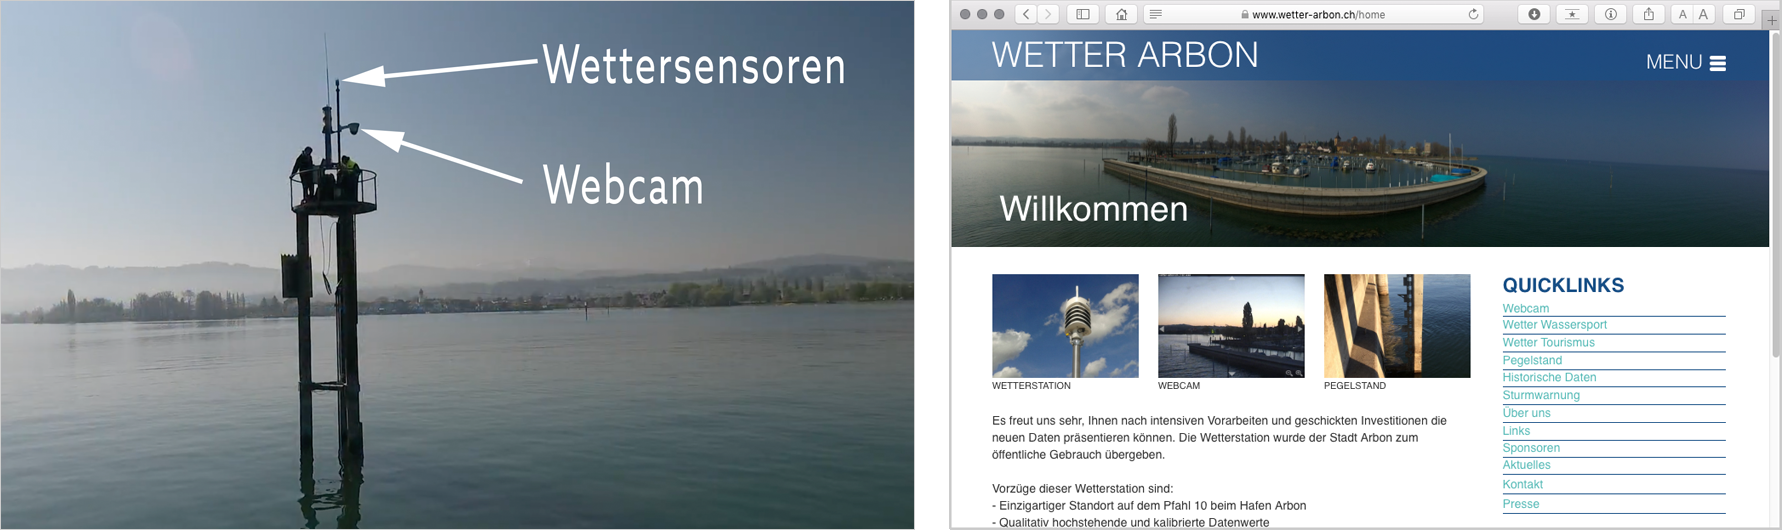
\includegraphics[width=1\linewidth]{img/kombi}
	\caption{Installation und Webseite der Wetterstation Arbon}
	\label{img:wetterstation}
\end{figure}

Die Bachelor-Arbeit hat das Ziel, die Wetterstation auf einen modernen, vollfunktionsfähigen Stand zu bringen. Die verschiedenen Arbeiten wurden in vier Blöcke zusammengefasst: Hardware, Webseite, Back end und Webcam. (vgl. Abb. \ref{img:module})

\vspace{5mm} %5mm vertical space

\begin{figure}[h!]
	\centering
	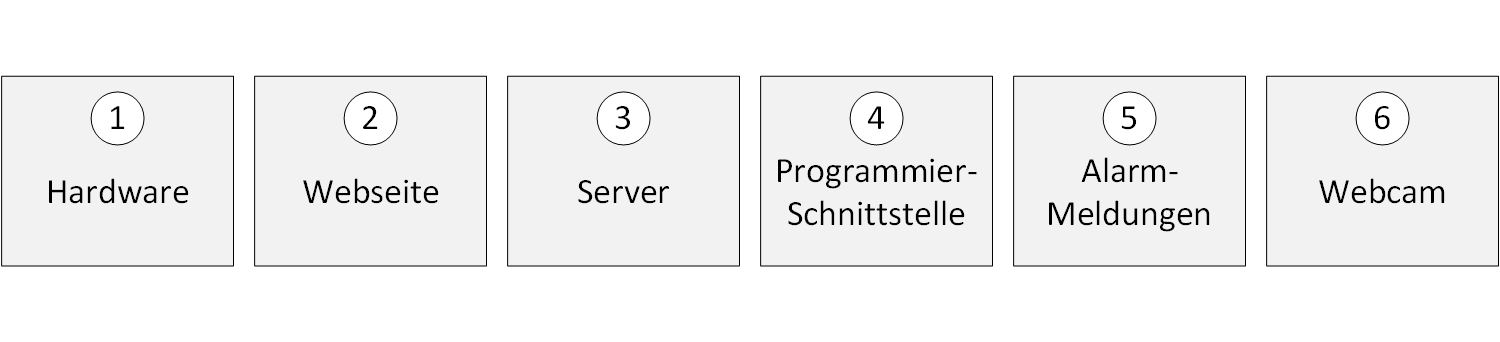
\includegraphics[width=0.8\linewidth]{img/module}
	\caption{Aufteilung in Arbeitsblöcke}
	\label{img:module}
\end{figure}


\newpage

\pagestyle{headings} % zeigt Kapitel in der Kopfzeile an
\section{Aufbau der Wetterstation und deren Sensoren}
Die Wetterstation Arbon verfügt über fünf Sensoren bzw. Sensor-Einheiten: Webcam, Kombi-Wettertransmitter, Wassertemperatur-Sensoren, Pegelsensor und Sonnenstrahlungssensor. Auf der Plattform im See befindet sich lediglich ein Schaltschrank mit Datenwandlern, keine Auswerteeinheit. Sämtliche Daten werden per TCP/IP über eine Glasfaserleitung an den landseitigen Server geschickt. Abbildung \ref{img:schaltschrank} zeigt den schematischen Aufbau der Komponenten im Schaltschrank und die angeschlossenen Sensoren. Die Stromversorgung ist der Übersicht halber nicht dargestellt. Der Pegel- und Strahlungssensor wurden während der Bachelor-Arbeit ersetzt beziehungsweise hinzugefügt. In den folgenden Kapiteln werden die neuen Sensoren und deren Funktionsweise erläutert.

\begin{figure}[htbp]
	\centering
	\fbox{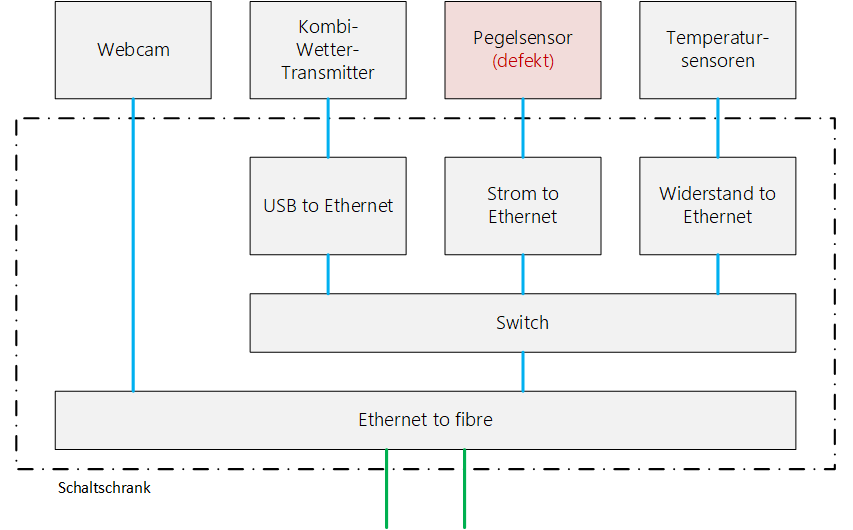
\includegraphics[width=\textwidth-2\fboxsep-2\fboxrule]{img/schaltschrank.png}}
	\caption{Hardware-Schema der Wetterstation}
	\label{img:schaltschrank}
\end{figure}




%% ############################################################################
%% Unterkapitel
%% ############################################################################
\subsection{Pegelsensor und Wellenhöhenmessung}
Die ursprüngliche Wetterstation verwendete einen hydrostatischen Drucksensor für die Messung des Wasserstands (Pegel). Der Drucksensor lieferte aber nach zehn Jahren Betrieb keine plausiblen Werte mehr, weshalb er ersetzt werden musste. Im Folgenden wird näher auf die möglichen alternativen Messprinzipien eingegangen und erklärt, wie der \emph{Pegel Konstanz} und die \emph{signifikante Wellenhöhe} definiert sind.

\subsubsection{Auswahl eines geeigneten Pegelsensors}
Für die Messung des Bodensee-Pegels wurden verschiedene Messprinzipien verglichen, mit dem Hintergedanken die Pegelmesswerte ebenfalls zur Messung der Wellenhöhe verwenden zu können. Die Zusammenfassung der Resultate ist in der Tabelle\,\ref{tbl:pegelsensoren} aufgelistet. TOF steht für \emph{time of flight} und beschreibt ein 3D-Kamerasystem. Die Einfachheit und Robustheit des hydrostatischen Sensors überwog, sodass der alte Drucksensor durch das gleiche Produkt ersetzt wurde.

\begin{table}[htbp!]
	\caption{Gegenüberstellung der verschiedenen Pegelmess-Prinzipien}
	\label{tbl:pegelsensoren}
	\setlength\extrarowheight{4pt} % for a more "open" look
	\begin{tabularx}{\textwidth}{|>{\RaggedRight\hspace{0pt}}p{3cm}||X|X|}
	\hline
	& \bfseries Vorteile
	& \bfseries Nachteile\\

	\hline
	\textbf{Hydrostatisch}
	&
	\begin{itemize}[nosep,leftmargin=*]
	\item einfache Auswertung
	\item mechanische Dämpfung
	\item sehr kleiner Energieverbrauch
	\end{itemize}
	&
	\begin{itemize}[nosep,leftmargin=*]
	\item anfällig auf Verschmutzung
	\item keine Wellenmessung möglich
	\end{itemize}\\

	\hline
	\textbf{Ultraschall}
	&
	\begin{itemize}[nosep,leftmargin=*]
	\item berührungslos
	\item geringer Energiebedarf
	\end{itemize}
	&
	\begin{itemize}[nosep,leftmargin=*]
	\item anfällig auf Wind
	\end{itemize}\\

	\hline
	\textbf{Radar}
	&
	\begin{itemize}[nosep,leftmargin=*]
	\item windunabhängig
	\item berührungslos
	\end{itemize}
	&
	\begin{itemize}[nosep,leftmargin=*]
	\item zu geringe Auflösung für Wellenhöhe
	\item hoher Energiebedarf
	\end{itemize}\\

	\hline
	\textbf{TOF}
	&
	\begin{itemize}[nosep,leftmargin=*]
	\item Wellenhöhe messbar
	\item berührungslos
	\end{itemize}
	&
	\begin{itemize}[nosep,leftmargin=*]
	\item komplexe Auswertung
	\end{itemize}\\

	\hline
	\textbf{Boje}
	&
	\begin{itemize}[nosep,leftmargin=*]
	\item Wellenhöhe messbar
	\end{itemize}
	&
	\begin{itemize}[nosep,leftmargin=*]
	\item wartungsintensiv
	\item Batteriebetrieb
	\end{itemize}\\

	\hline
	\end{tabularx}
\end{table}

\subsubsection{Definition des Pegel Konstanz}
Die Uferlinie des Bodensees wurde 1990 von der IGKB\footnote{IGKB: Internationalen Gewässerschutzkommission für den Bodensee} bei Mittelwasserstand festgelegt. Der Pegelstand in Konstanz ist ein Relativmaß. Er bezieht sich auf den Pegelnullpunkt, der in Konstanz bei 391,89m ü NN liegt. Der Pegel Romanshorn gibt die geodätische Höhe des Wasserstandes in Meter über Meer wieder\footnote{\url{http://www.bodensee-hochwasser.info/IGKB/umrechnung.html}}. Der Zusammenhang der verschieden Pegelgrössen ist in Abbildung\,\ref{img:pegelKonstanz} dargestellt. Links oben (violett) befindet sich die Skala für den Pegel Konstanz. Die offizielle Hochwassermarke liegt bei einem Pegel von 4,80 Metern.

\begin{figure}[htbp!]
	\centering
	\fbox{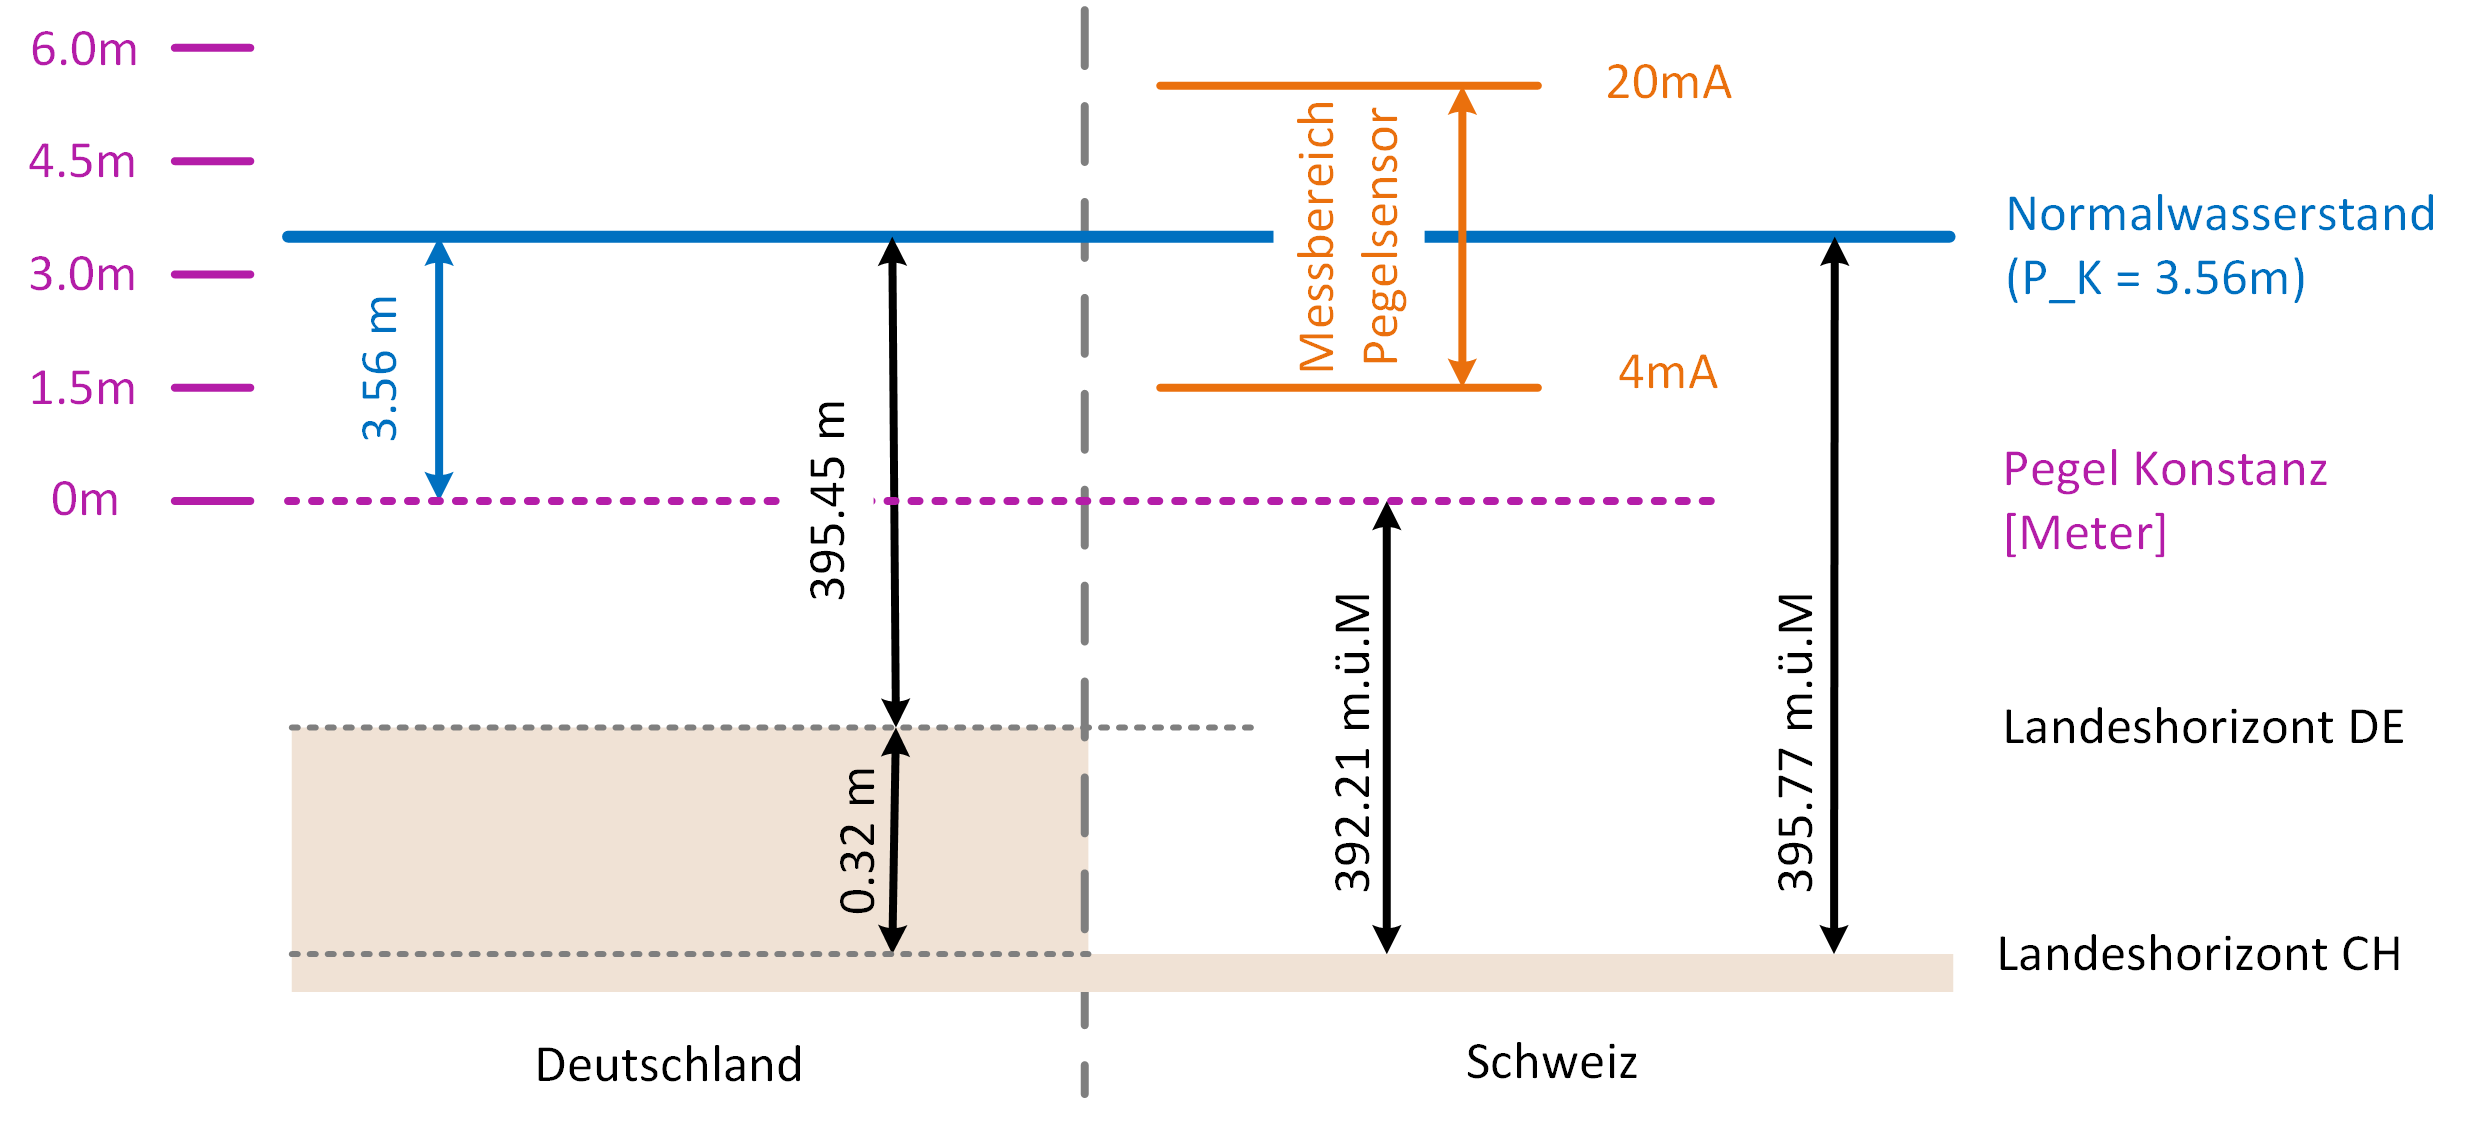
\includegraphics[width=\textwidth-2\fboxsep-2\fboxrule]{img/pegelKonstanz}}
	\caption{Berechnung des Pegel Konstanz und Messbereich des Sensors}
	\label{img:pegelKonstanz}
\end{figure}

\noindent
Der Pegelsensor liefert einen Strom von 4...20\,mA bei einer Messhöhe von 4\,Meter. Der Pegelsensor ist 1.75\,Meter über dem Pegelnullstand angebracht.
Die Berechnung des Pegel Konstanz aus dem Messwert erfolgt demnach gemäss der Formel \ref{eq:Pegelformel}. Aus technischen Gründen ist 1.75\,m bzw. 5.75\,m der tiefste bzw. höchste von der Wetterstation messbare Pegel, wie in Formel\,\ref{eq:Pegelmin} und \ref{eq:Pegelmax} berechnet.

\begin{equation}
\label{eq:Pegelformel}
P_{K} = m*x + q = 4/16 * x + 0.75
\end{equation}

\begin{equation}
\label{eq:Pegelmin}
P_{g,u}= P_{K}(x=4)= 4*0.25 + 0.75 = 1.75
\end{equation}

\begin{equation}
\label{eq:Pegelmax}
P_{g,o} = P_{K}(x=20)= 20*0.25 + 0.75 = 5.75
\end{equation}

wobei:
\begin{conditions}
P_{K}    &  Pegel Konstanz [m]\\
P_{g,u}   &  Tiefster messbarer Pegel [m]\\
P_{g,o}   &  Höchster messbarer Pegel [m]\\
x        &  Messwert [mA]\\
m        &  Auflösung des Sensors [m/mA] (0...4m bei 4...20mA)\\
q        &  Offset [m] \\
\end{conditions}

\noindent
Der Pegelsensor ist an einem Web-Interface angeschlossen, welches den Strom-Messwert über eine Web-Schnittstelle zur Verfügung stellt. Der aktuelle Messwert kann so bequem mittels GET-Abfrage aufgerufen werden, wie in Listing\,\ref{lst:curlPegel} aufgezeigt. Da das Web-Interface nur schwach (Passwortabfrage in Klartext) gegen unerwünschte Zugriffe geschützt sind, wurde die Firewall der Wetterstation so konfiguriert, dass nur vom Hosting-Server aus die Abfrage durchgeführt werden kann (IP-Einschränkung).

\vspace{3mm}
\begin{lstlisting}[label=lst:curlPegel,caption=Abfrage des Pegelsensor-Wertes über das Hostpoint-Termianl, language=Python, style=htmlcssjs]
[igwetter:] $ curl http://webcam.wetter-arbon.ch:50506/single1
11,748 mA
\end{lstlisting}
\vspace{3mm}

\subsubsection{Definition der signifikaten Wellenhöhe}
Ursprünglich war geplant mit dem Pegelsensor ebenfalls die Wellenhöhe zu messen. Dies ist aber mit dem gewählten Pegelsensor bzw. dessen Montage nicht möglich. Das Einbaurohr wirkt als Tiefpass-Filter und verunmöglicht die Messung von schnellen Wassersäuleänderungen. Nichtsdestotrotz und im Hinblick auf eine allfällige Erweiterung der Wetterstation um einen Wellenhöhensensor soll hier kurz die Definition der signifikaten Wellenhöhe erläutert werden.

Als Seegang bezeichnet man die winderzeugten Oberflächenwellen des Meeres. Da sich der Seegang in der Natur als eine Überlagerung vieler Einzelwellen darstellt, werden zu dessen Beschreibung statistische Größen wie z.B. die signifikante Wellenhöhe verwendet. Die Definition einer signifikanten Wellenhöhe geht auf die visuelle Bestimmung einer charakteristischen, den Seegang beschreibenden Wellenhöhe zurück. Die signifikante Wellenhöhe wird gemäss der \emph{List of sea state parameters}\cite{1986Iahr} definiert als die mittlere Wellenhöhe von 33\,\% höchsten Wellen in einem repräsentativen Zeitraum (z.B. 20\,Minuten).

%% ############################################################################
%% Unterkapitel
%% ############################################################################
\subsection{Wassertemperatur-Sensoren}
Die Wetterstation verfügt über acht Wasser-Temperatursensoren (PT100-Elemente), die im Abstand von 0.5\,m in einem Rohr angebracht sind. Die offizielle Wassertemperatur wird einen Meter unter der Wasseroberfläche gemessen. Für Schwimmer ist aber die Temperatur auf einem halben Meter unter der Wasseroberfläche interessanter, weshalb dieser Wert ebenfalls ausgelesen und gespeichert wird. Das Schwimmbad Arbon bezieht bereits heute für ihre Webseite\footnote{\url{https://www.schwimmbad-arbon.ch}} die Wassertemperatur von der Wetterstation.
% \Diskussionspunkt{- Wo ist Wassertemperatur definiert? }

\begin{figure}[htbp]
	\centering
	\fbox{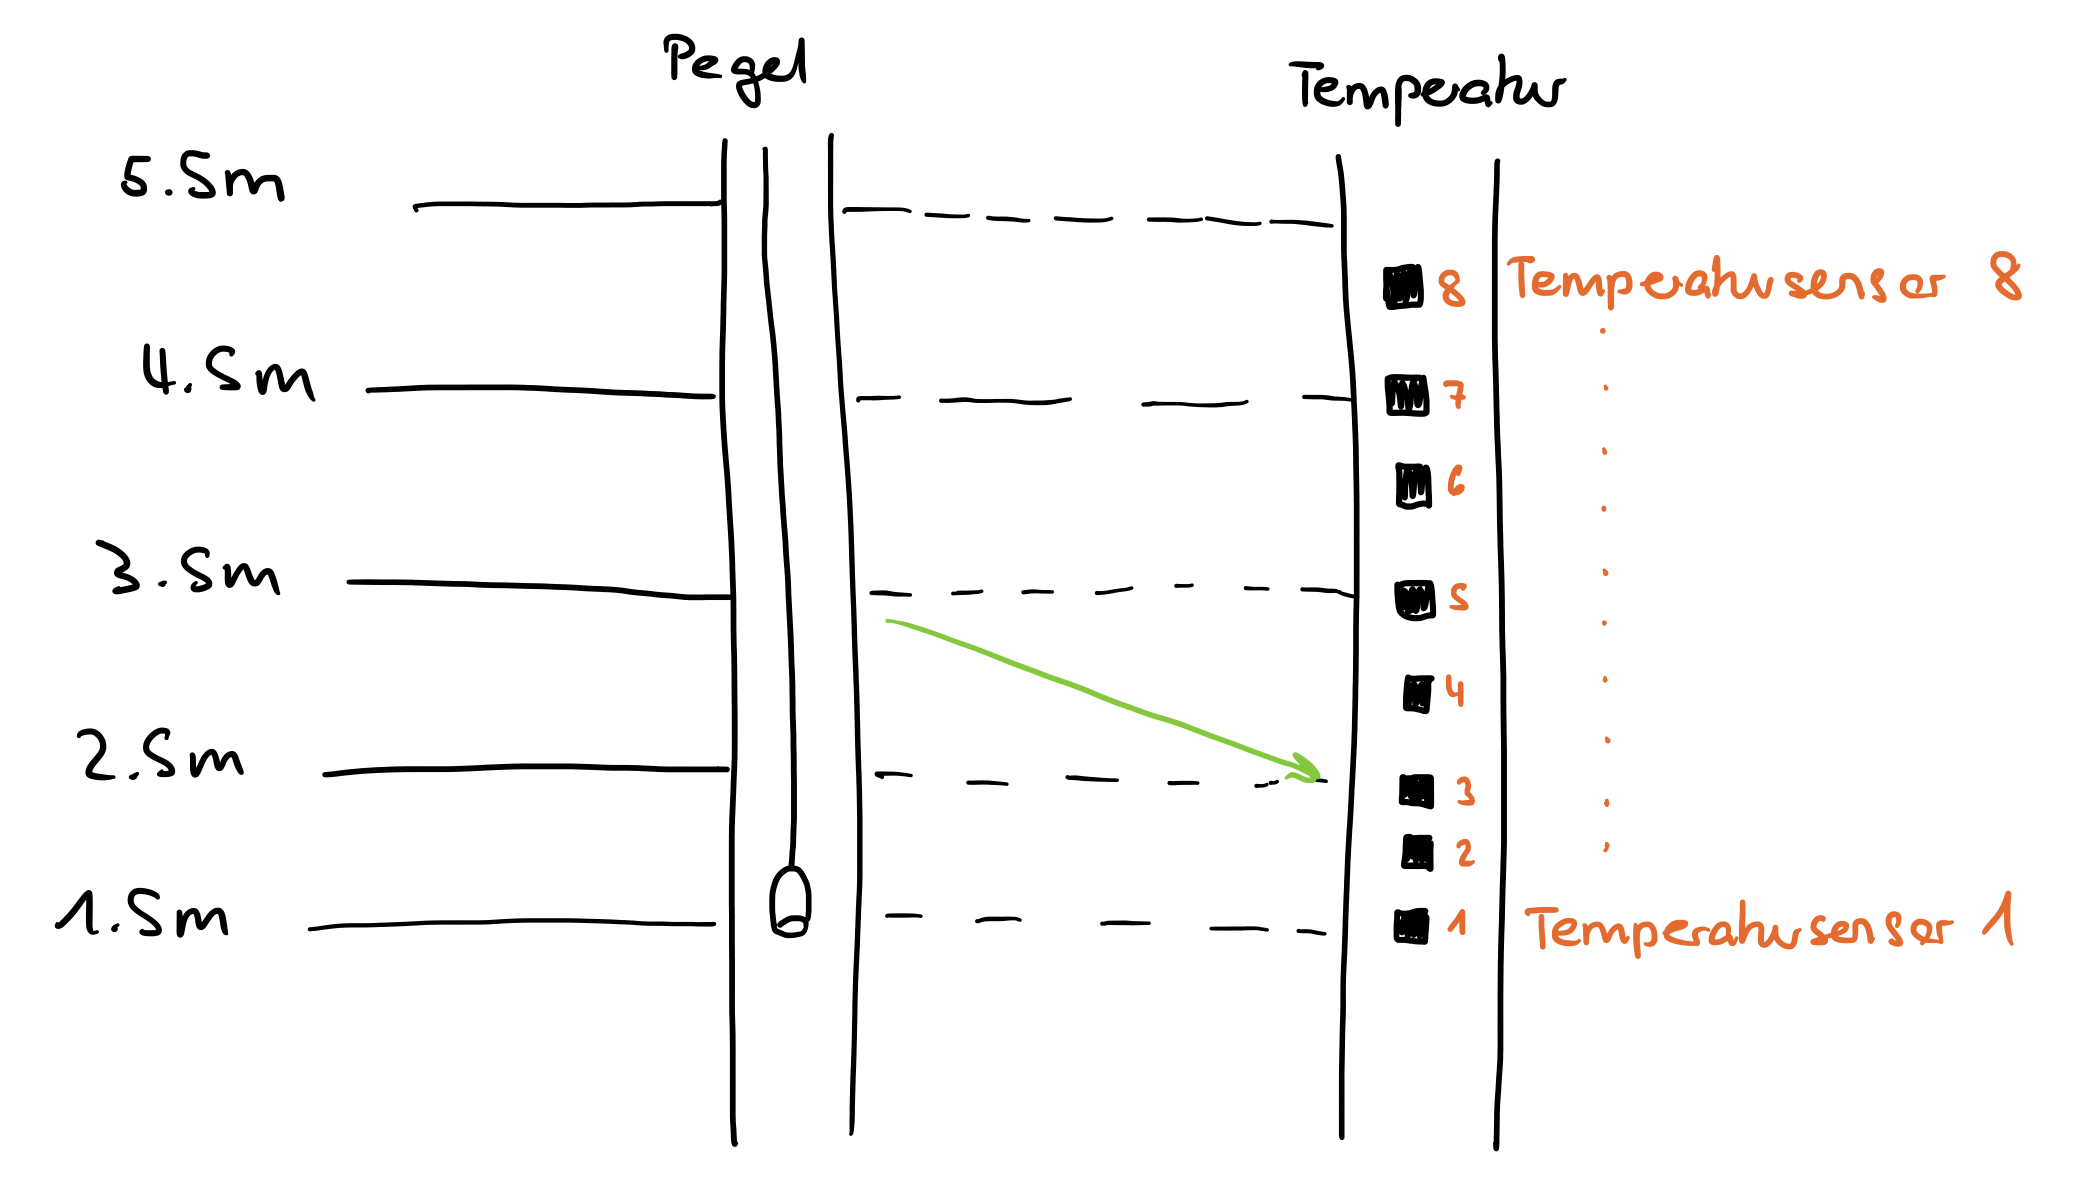
\includegraphics[width=\textwidth-2\fboxsep-2\fboxrule]{img/wassertempsensoren}}
	\caption{Zusammenhang zwischen Pegel und PT100-Temperaturwiderständen}
	\label{img:wassertempsensoren}
\end{figure}

\subsubsection{Auswahl des richtigen Temperatursensors anhand des Pegels}
Damit der richtige Temperatursensor ausgewählt werden kann, muss der Pegel bekannt sein. Abbildung \ref{img:wassertempsensoren} zeigt das Prinzip schematisch auf. Mittels Cronjob werden sämtliche Temperatursensoren ausgelesen und in einem Array gespeichert. Anschliessend wird mit Hilfe des Pegelwerts der korrekte Wert entnommen, wie in Listing \ref{lst:tempSelect} beispielhaft aufgezeigt.

\begin{lstlisting}[label=lst:tempSelect,caption=Auswahl des richtigen Temperatursensors, language=Python, style=py]
if waterlevel >= 3.5 and waterlevel <= 4.0:
    watertemperature100cm  = float(temperatureArray[3])
    watertemperature50cm   = float(temperatureArray[4])
\end{lstlisting}




\subsubsection{Annäherung des defekten PT100-Widerstands}
Die Temperatursensoren waren mehrere Jahre nicht in Betrieb. Zur Kontrolle wurden deshalb während sechs Wochen alle Temperaturdaten aufgezeichnet. Ein Auszug der Messdaten ist in Abbildung \ref{img:tempSensoren} dargestellt. Es lässt sich erkennen, dass sich die Sensoren\,1 bis 4 im Wasser, und die Sensoren\,6 bis 8 über Wasser befinden. Beim Sensor\,5 ist nicht klar, ob er im oder über dem Wasser ist. Auf Grund der Messdaten lässt sich auch kein konstanter Offset gegenüber den benachbarten Sensoren ermitteln.

\begin{figure}[htb!]
	\centering
	\fbox{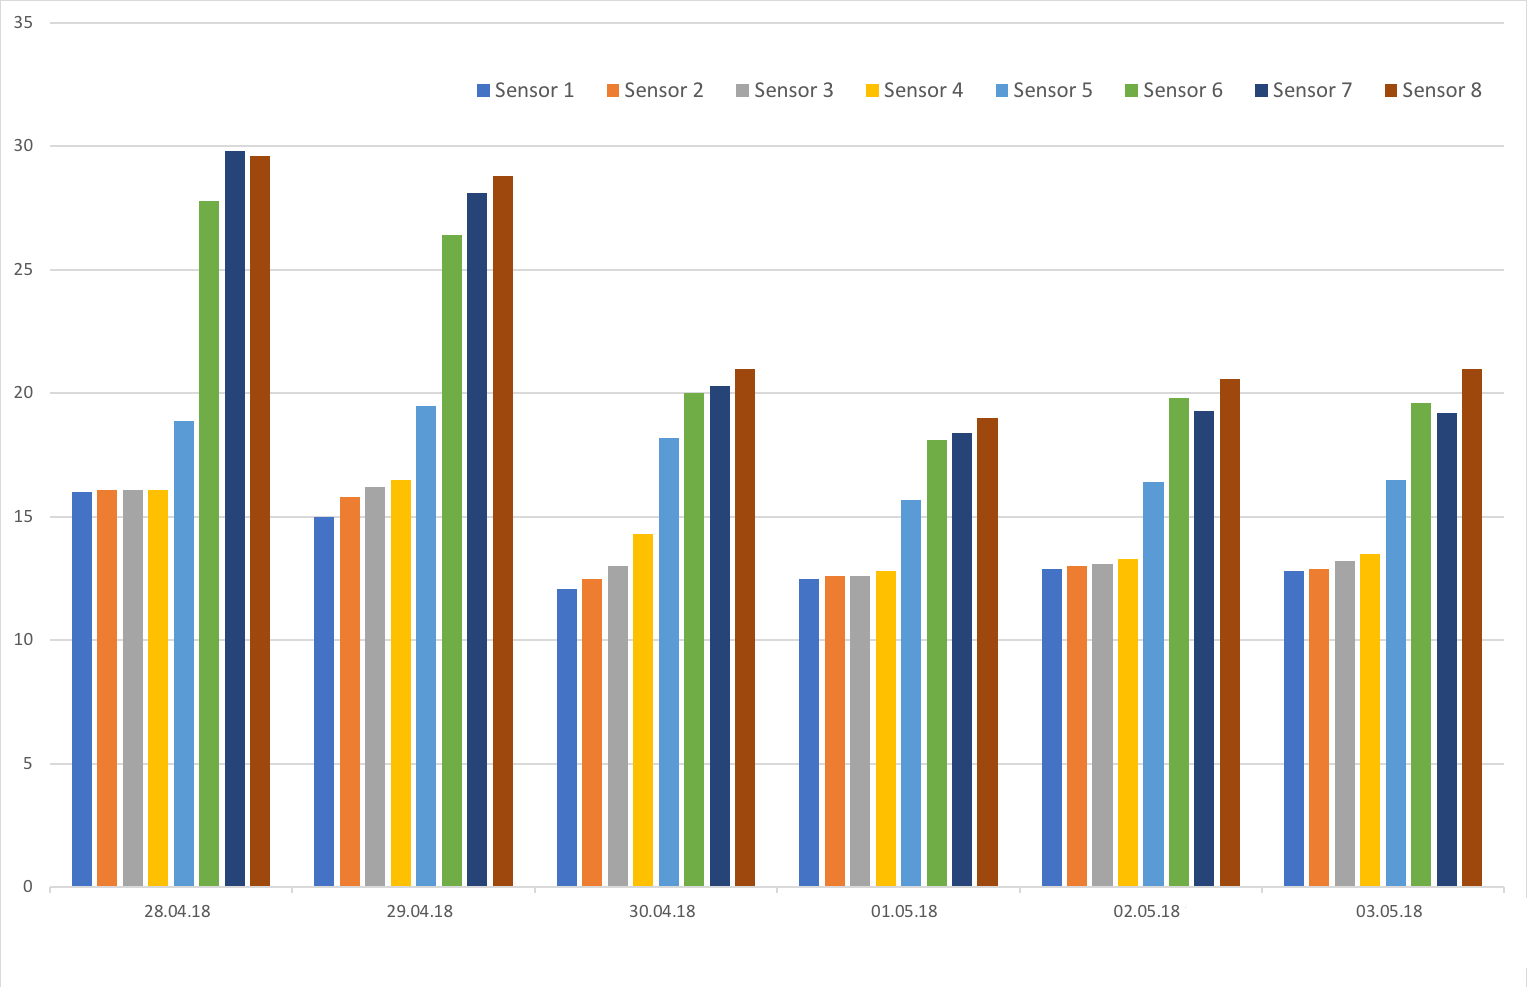
\includegraphics[width=\textwidth-2\fboxsep-2\fboxrule]{img/tempSensoren}}
	\caption{Messreihe aller Temperatursensoren}
	\label{img:tempSensoren}
\end{figure}

\noindent
Der fehlende bzw. falsche Wert wurde trotzdem durch einen Offset angenähert. Ein Offset von drei Grad hat sich als meistens korrekt erwiesen. Der Offset wird direkt beim Auslesen der Temperaturdaten abgezogen, wie in Listing \ref{lst:tempOffset} aufgezeigt.

\vspace{3mm}
\begin{lstlisting}[label=lst:tempOffset,caption=Offset des defekten Temperatusensors, language=Python, style=py]
offset = -3  # [Grad]
temperatureArray[4] = float(temperatureArray[4]) + offset
\end{lstlisting}


%% ############################################################################
%% Unterkapitel
%% ############################################################################
\subsection{Sonnenstrahlungssensor}
Die Sonnenscheindauer dient der näherungsweisen Bestimmung der Sonneneinstrahlung an einem bestimmten Ort und gibt gleichzeitig Hinweise auf Zeit und Stärke der Bewölkung. Sie diente ursprünglich der Charakterisierung von Kurorten. Dabei wurde die psychologische Wirkung von Sonnenlicht auf das menschliche Wohlbefinden hervorgehoben. Auch heute noch werden die Sonnenstunden verwendet, um touristische Ziele zu fördern.

\noindent
Zur Messung der Sonnenstunden gibt es gemäss \emph{Guide to Meteorological Instruments and Methods of Observation (WMO)}~\cite{WMO2014Gtmi} fünf Messprinzipien, wobei die pyranometrische Methode die einfachste und kostengünstigste Methode darstellt. Dabei misst ein Pyranometer die Globalstrahlung\,$G$, welche anschliessend zur Abschätzung der Sonnenscheindauer verwendet wird. Das Messprinzip des Pyranometers und die Berechnung der Sonnenstunden werden im Folgenden erklärt.

\subsubsection{Funktionsprinzip eines Pyranometers}
Das Pyranometer basiert auf dem Messprinzip eines Thermoelements. Die eintreffende Strahlung trifft auf einen Absorber, welcher erwärmt wird. Die Wärme fliesst dann über das Gehäuse an die Umgebung ab (siehe Abbildung\,\ref{img:pyranometer}. Die Strahlungsleistung ist dabei proportional zum Wärmestrom beziehungsweise zur Temperaturdifferenz vom Absorber zum Gehäuse. Die Temperaturdifferenz wird mit Thermoelementen gemessen. Um die Signalspannung zu erhöhen, werden mehrere Thermoelemente in Reihe zu einer Thermosäule geschalten. Durch das thermische Messprinzip ist ein Pyranometer träge. Die Verzögerung liegt bei wenigen Sekunden.

\begin{figure}[htbp]
	\centering
	\fbox{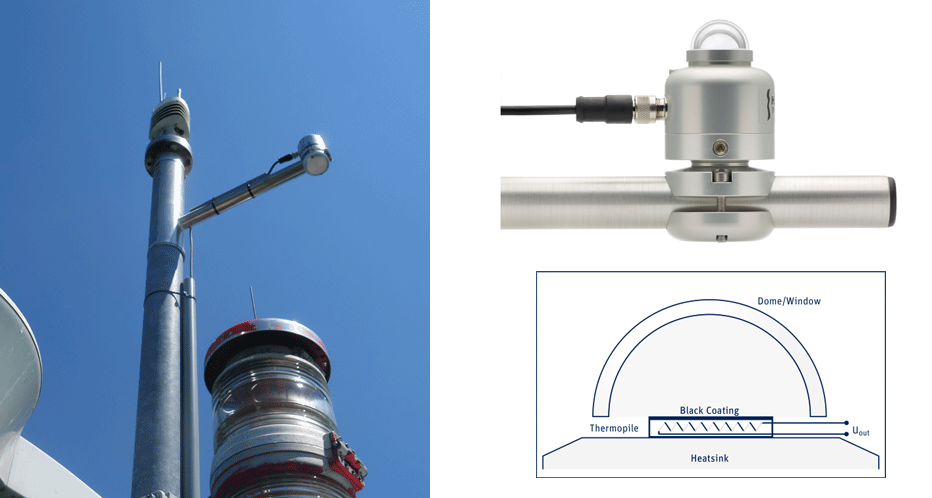
\includegraphics[width=\textwidth-2\fboxsep-2\fboxrule]{img/pyranometer.png}}
	\caption{Montageort und \href{http://www.kippzonen.com/News/572/The-Working-Principle-of-a-Thermopile-Pyranometer}{Funktionsprinzip} eine Pyranometers }
	\label{img:pyranometer}
\end{figure}


\subsubsection{Berechnung der Sonnenscheindauer}
Die Sonnenscheindauer (SD) kann aus den minütlichen Messwerten der Globalstrahlung\,$G$ berechnet werden~\cite{WMO2014Gtmi}. Dazu muss zuerst der Schwellwert\,$G_{thr}$, wie in der Formel\,\ref{eq:Sonnenstunden} dargestellt, berechnet werden. Der Schwellwert ist das Produkt aus mehreren Parametern, welche vom Standort und der Sonnenposition abhängig sind. Der Zähler für die Sonnenstunden wird um eine Minute erhöht, wenn der Messwert grösser ist als der Schwellwert und der Sonnenwinkel mindestens 3 Grad beträgt.

\vspace{3mm}
\begin{equation}
\label{eq:Sonnenstunden}
G_{thr} = A + B * cos \left(\frac{360*d}{24*365}\right) * 1080 * sin(h)^{1.25}
\end{equation}
\vspace{3mm}

wobei:
\begin{conditions}
G_{thr}  &  Schwellwert der Globalstrahlung \\
d        &  Laufende Stunde seit Anfang Jahr \\
h        &  Elevationswinkel der Sonne in Grad \\
A        &  empirisch bestimmter Koeffizient (0.65) \\
B        &  empirisch bestimmter Koeffizient (Saisonalität) (0.15) \\
\end{conditions}

\noindent
Zur Bestimmung der beiden Koeffizienten $A$ und $B$ konnte auf die Messwerte des NTB in Buchs zurückgegriffen werden. Da die Strahlungsintensität von Buchs und Arbon vergleichbar sind (gleiche geografische Breite und Höhe), wurden die Koeffizienten direkt übernommen. Abbildung\,\ref{img:radiation} zeigt die Darstellung von Sonnenscheindauer und Strahlung, sowie deren Verlauf über die letzten beiden Tage, wie sie auf der Webseite angezeigt werden.

\begin{figure}[htbp]
	\centering
	\fbox{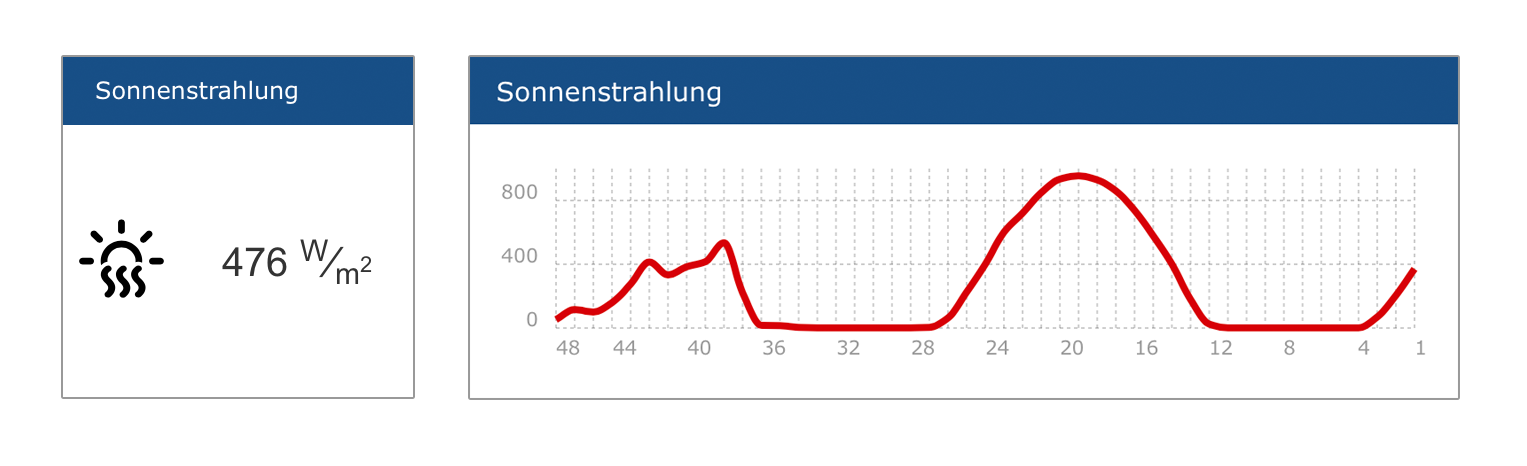
\includegraphics[width=\textwidth-2\fboxsep-2\fboxrule]{img/radiation}}
	\caption{Darstellung des aktuellen Messwerts und des Strahlungsverlaufs}
	\label{img:radiation}
\end{figure}

\subsubsection{Verwendung für PV-Anlagen}
Das webbasierte Tool PVGIS\footnote{\url{http://re.jrc.ec.europa.eu/pvgis/apps4/pvest.php}}, welches durch das europäische \emph{Joint Research Centre} (JRC) entwickelt wurde, ist ein beliebtes Tool, wenn es darum geht den Ertrag einer PV-Anlage vorherzusagen. Die Daten basierend auf der Interpolationen von Messungen von diversen Boden-Messstationen. Es liegt nahe diese Berechnung mit unseren Messwerten zu vergleichen. PVGIS berechnet für den Standort Arbon im Monat July Strahlungswerte von bis zu $900 \nicefrac{W}{m_2}$, gemäss Abbildung\,\ref{img:pvgis}.

\begin{figure}[htb!]
	\centering
	\fbox{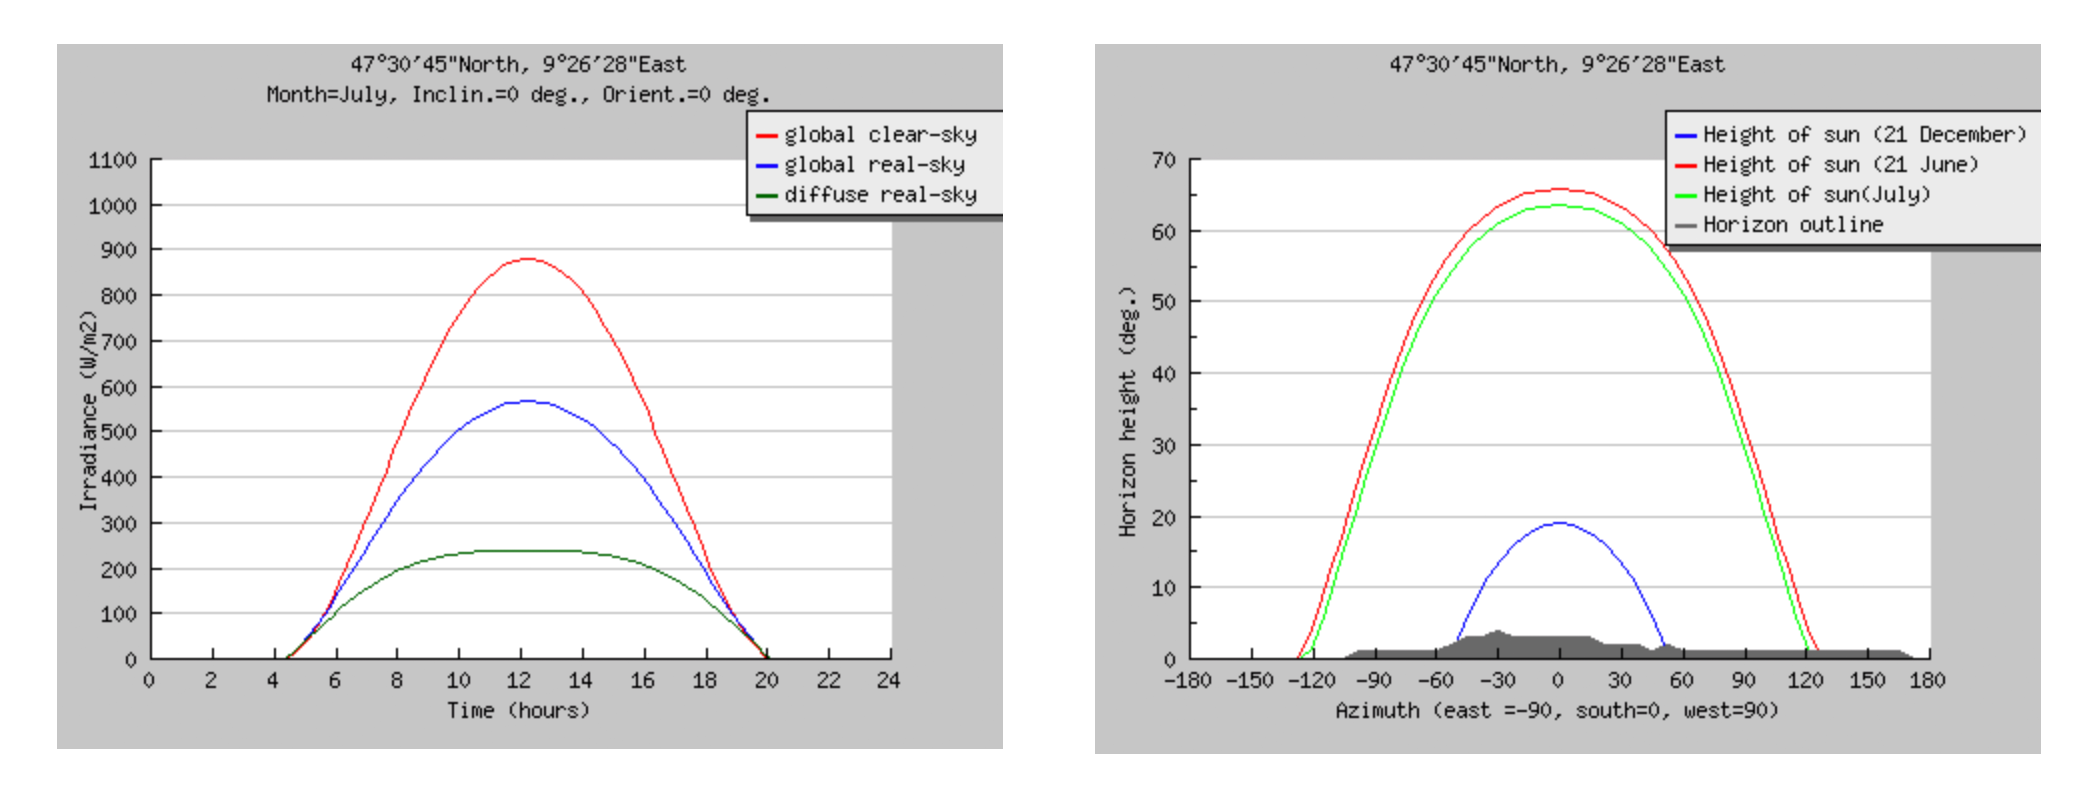
\includegraphics[width=\textwidth-2\fboxsep-2\fboxrule]{img/pvgis}}
	\caption{Interplolierte Strahlungvorhersage und Sonnenwinkel für Arbon}
	\label{img:pvgis}
\end{figure}

\section{Grafische Benutzeroberfläche (Website)}
Die bisherige Anzeige der Wetterdaten basiert auf Adobe Flash, was nicht von allen Browsern unterstützt wird (siehe Fachmodul-Bericht). Die neue (2014) HTML5-Spezifikation ermöglicht es dynamische Grafiken zu erzeugen, die nativ von allen Web-Browsern dargestellt werden können.


%% ############################################################################
%% Unterkapitel
%% ############################################################################
\subsection{Nutzungsanalyse der Website mittels Google Analytics}
\label{subsec:googleAnalytics}
Zuerst wurden die Zugriffsdaten auf die bestehende Webseite mittels Google Analytics analysiert. Als Zeitraum wurde das gesamte Jahr 2017 gewählt. Auf der bisherigen Webseite gab es zwei Unterseiten \textit{Wetter Tourismus} und \textit{Wetter Wassersport}, die sich aber nur gering voneinander unterscheiden z.B. in der Wahl der Einheit der Windgeschwindigkeit (km/h vs. kn). Die Zugriffsdaten sind in Abbildung \ref{img:google_mobile} dargestellt. Darin lässt sich erkennen, dass der Anteil an mobilen Geräten zwischen 50\% und 80\% beträgt. Dies wiederspiegelt den Trend zum mobilen Internet und zeigt wie wichtig die mobile Version einer Webseite ist. Dies geht soweit, dass sogar die mobile Seite als Ausgangspunkt für die Entwicklung der Homepage dient nach dem Designkonzept \textit{Mobile First}.

\begin{figure}[h!]
  \fbox{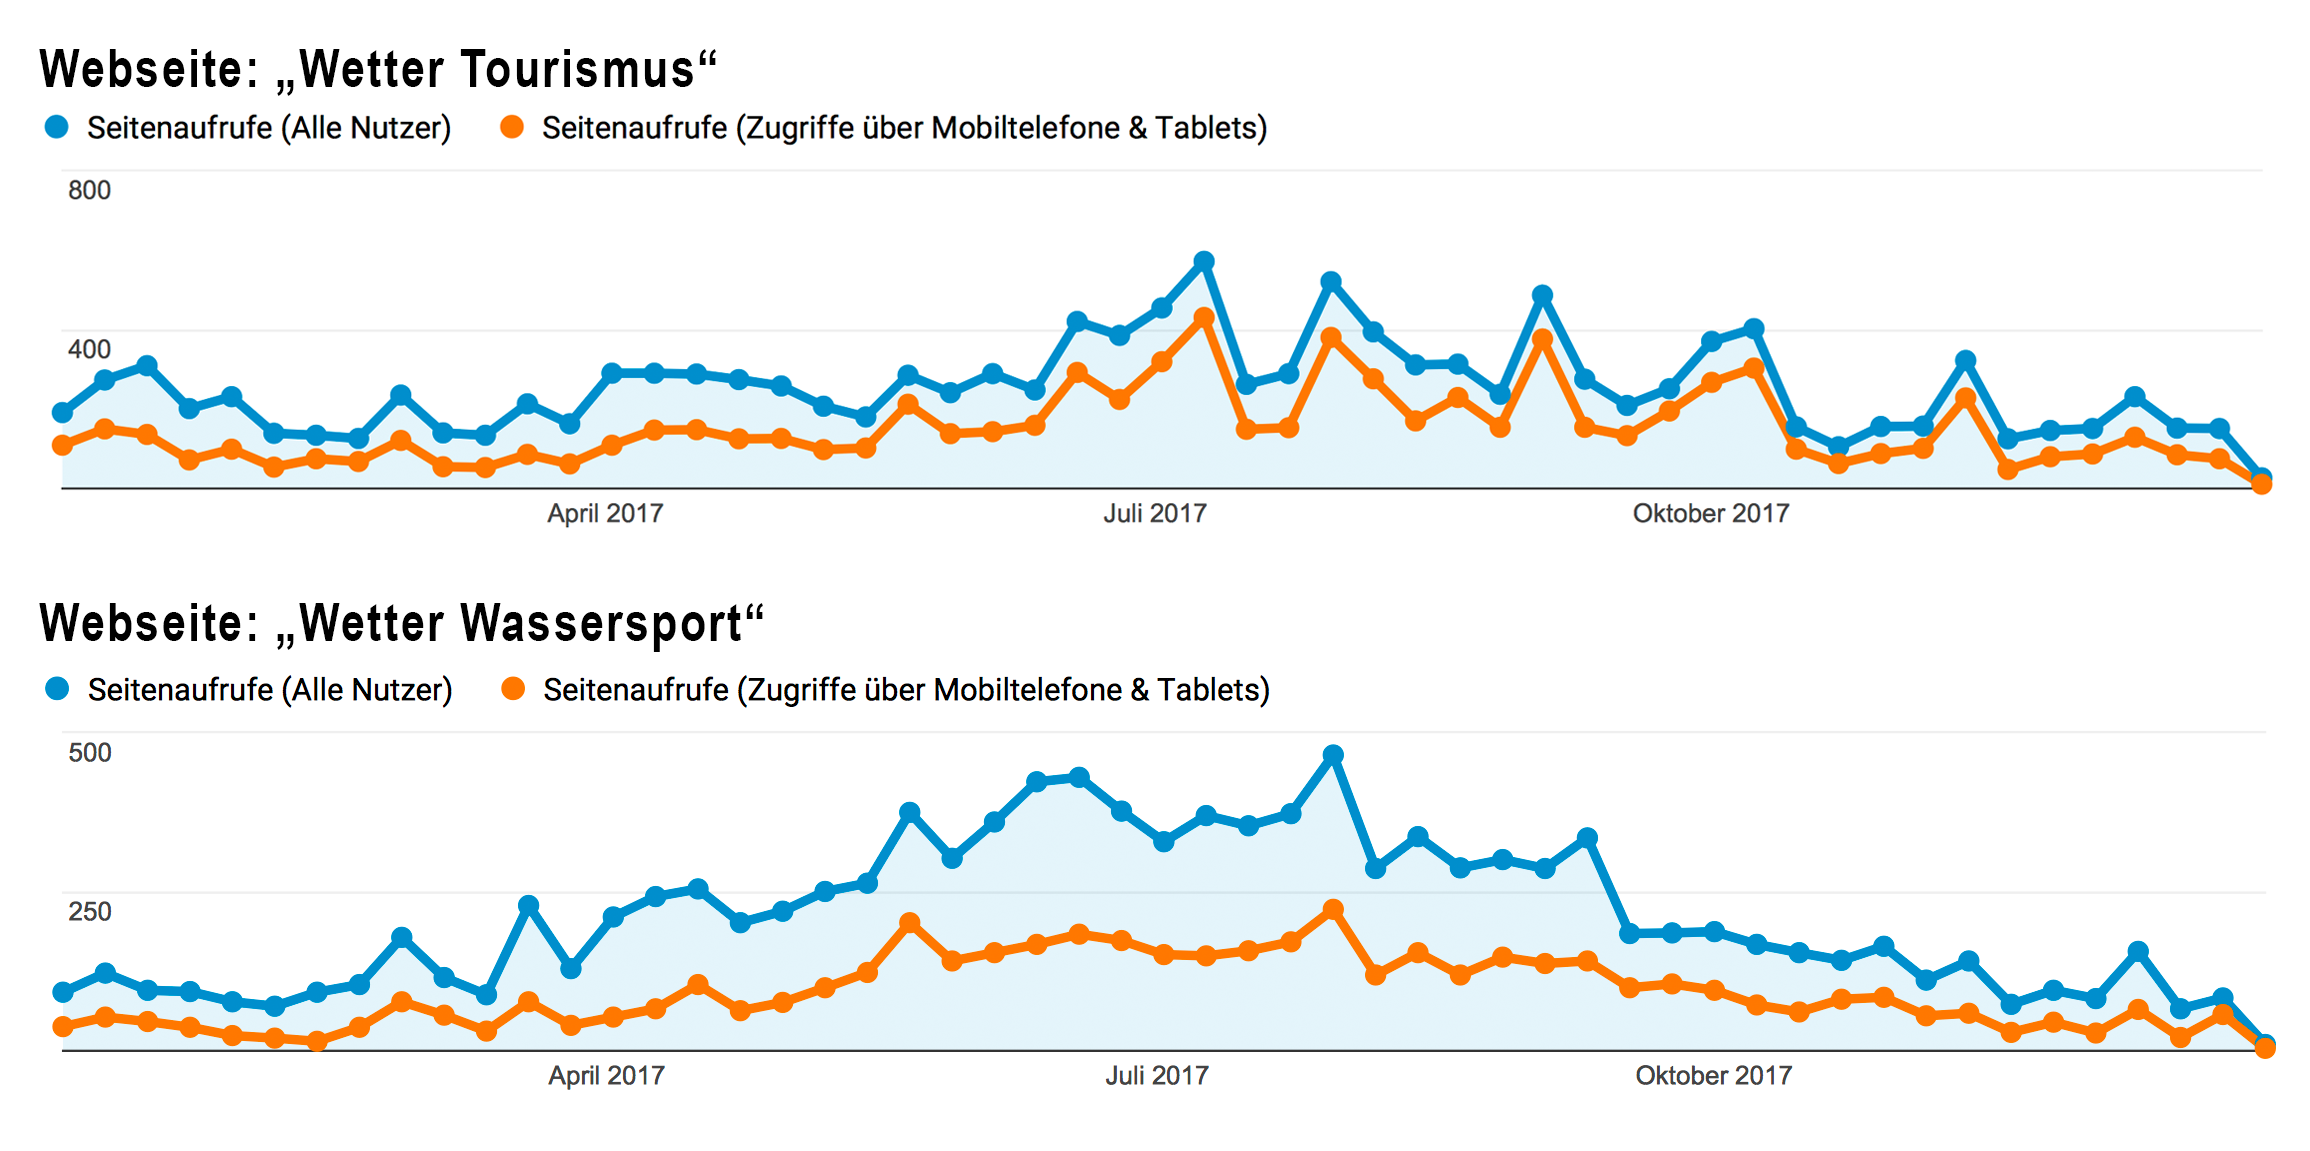
\includegraphics[width=\textwidth-2\fboxsep-2\fboxrule]{img/google_mobile}}
	\centering
	\caption{Anteil der mobilen Zugriffe auf die Wetterwebseite}
	\label{img:google_mobile}
\end{figure}

Es lässt sich ebenfalls erkennen welche Browser am häufigsten verwendet werden und welches die beliebteste Seite der Website ist, wie in Abbildung \ref{img:google_browser} dargestellt.

\begin{figure}[h!]
	\centering
	\fbox{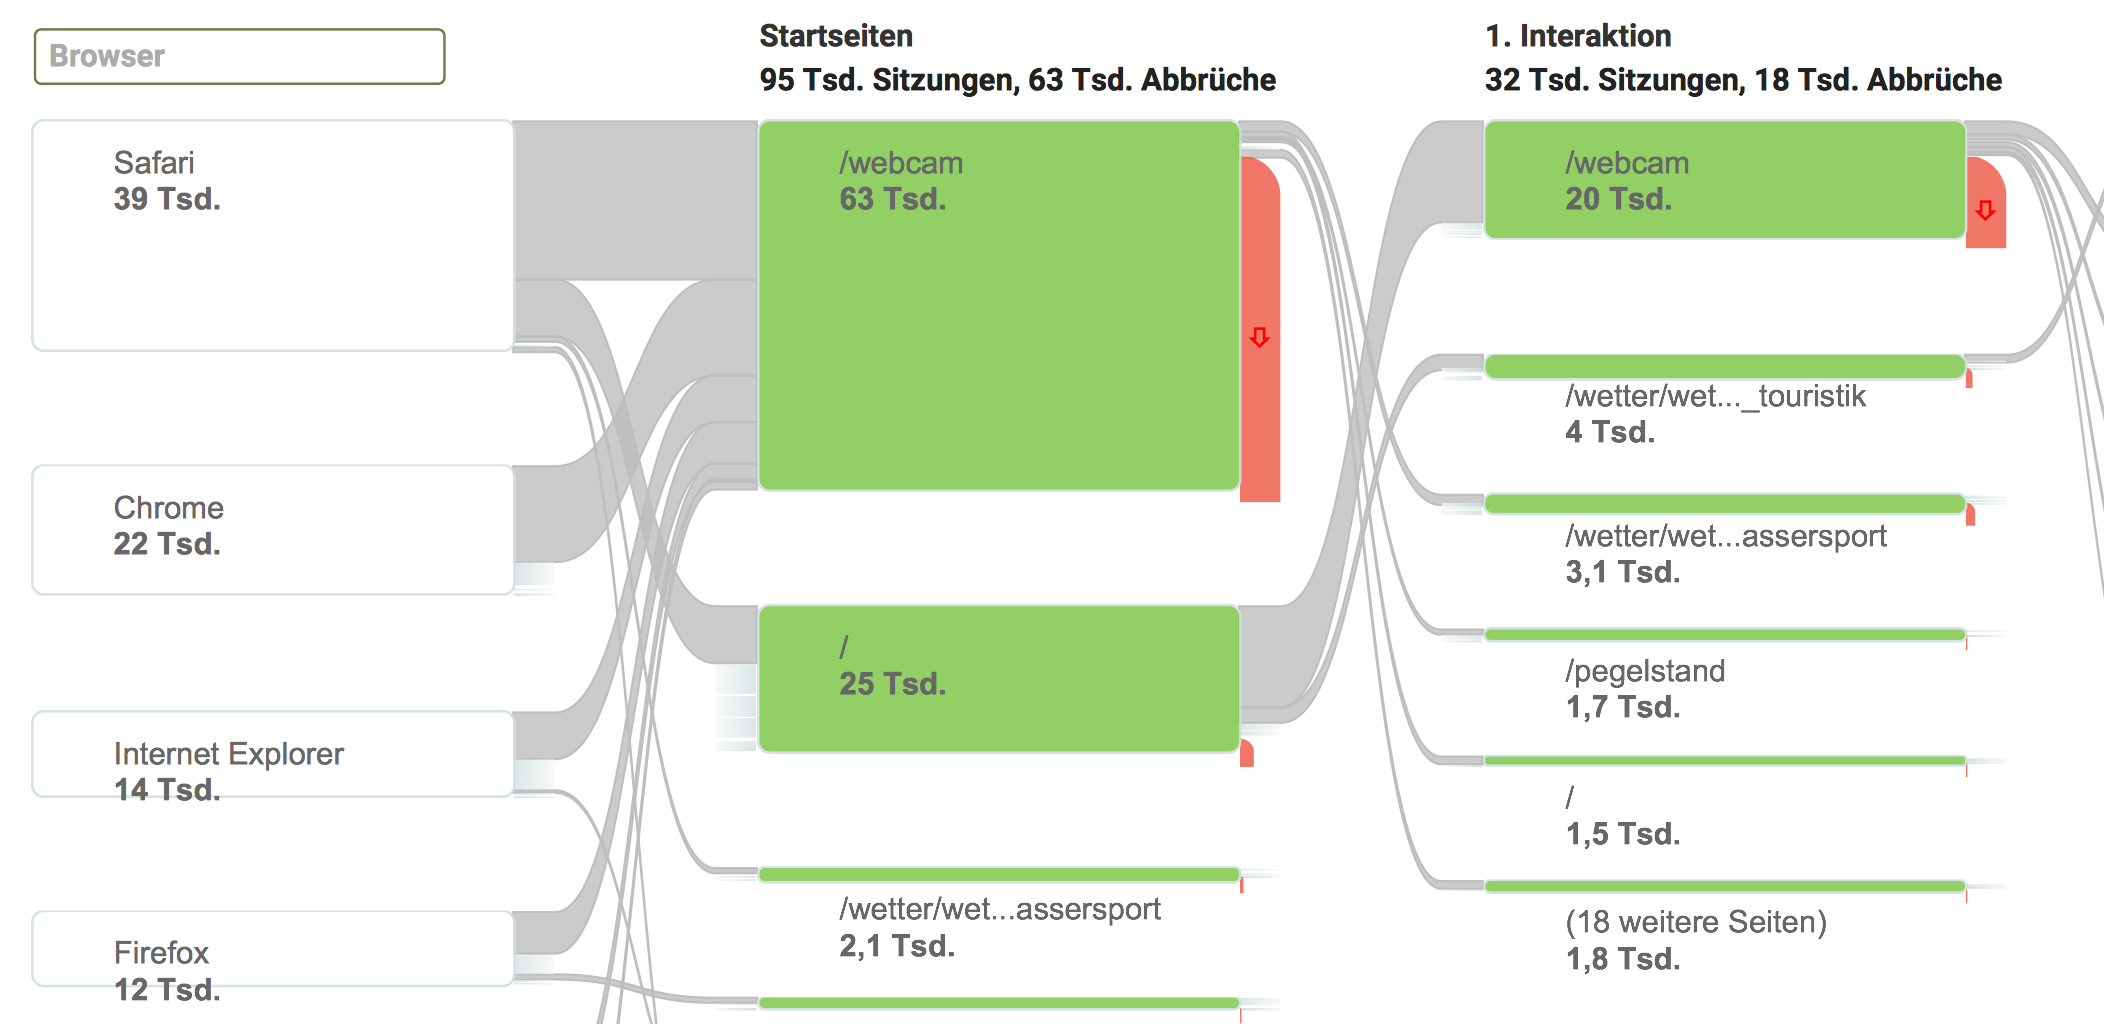
\includegraphics[width=\textwidth-2\fboxsep-2\fboxrule]{img/google_browser}}
	\caption{Verwendete Browser und Beliebtheit der Seiten}
	\label{img:google_browser}
\end{figure}



%% ############################################################################
%% Unterkapitel
%% ############################################################################
\subsection{Konzeption der crossplattformfähigen Benutzeroberfläche}
Wie im Abschnitt \ref{subsec:googleAnalytics} aufgezeigt werden bereits heute 50\% bis 80\% der Aufrufe von mobilen Geräten ausgeführt, Tendenz steigend. Es ist deshalb naheliegend das mobile Design als Startpunkt zu verwenden. Diese Vorgehensweise nennt sich \textit{Mobile First}. Es ist ein Designkonzept, das von Luke Wroblewski 2009 das erste Mal vorgeschlagen wurde. Die optimale Darstellung einer Website auf mobilen Endgeräten hat dabei oberste Priorität. Bei Mobile First beginnt der Designer mit dem Mobile-Design und arbeitet sich dann schrittweise zur grösseren Desktop-Version vor. Die \flqq Mobile Web Best Practices\frqq \footnote{ \url{https://www.w3.org/TR/mobile-bp}} des W3C empfiehlt zudem, dass sämtliche Informationen, die in der Desktop-Version zur Verfügung stehen, auch von der mobilen Seite aufgerufen werden können. Dieser Grundsatz nennt sich \textit{One Web Design}.

\begin{figure}[h!]
  \fbox{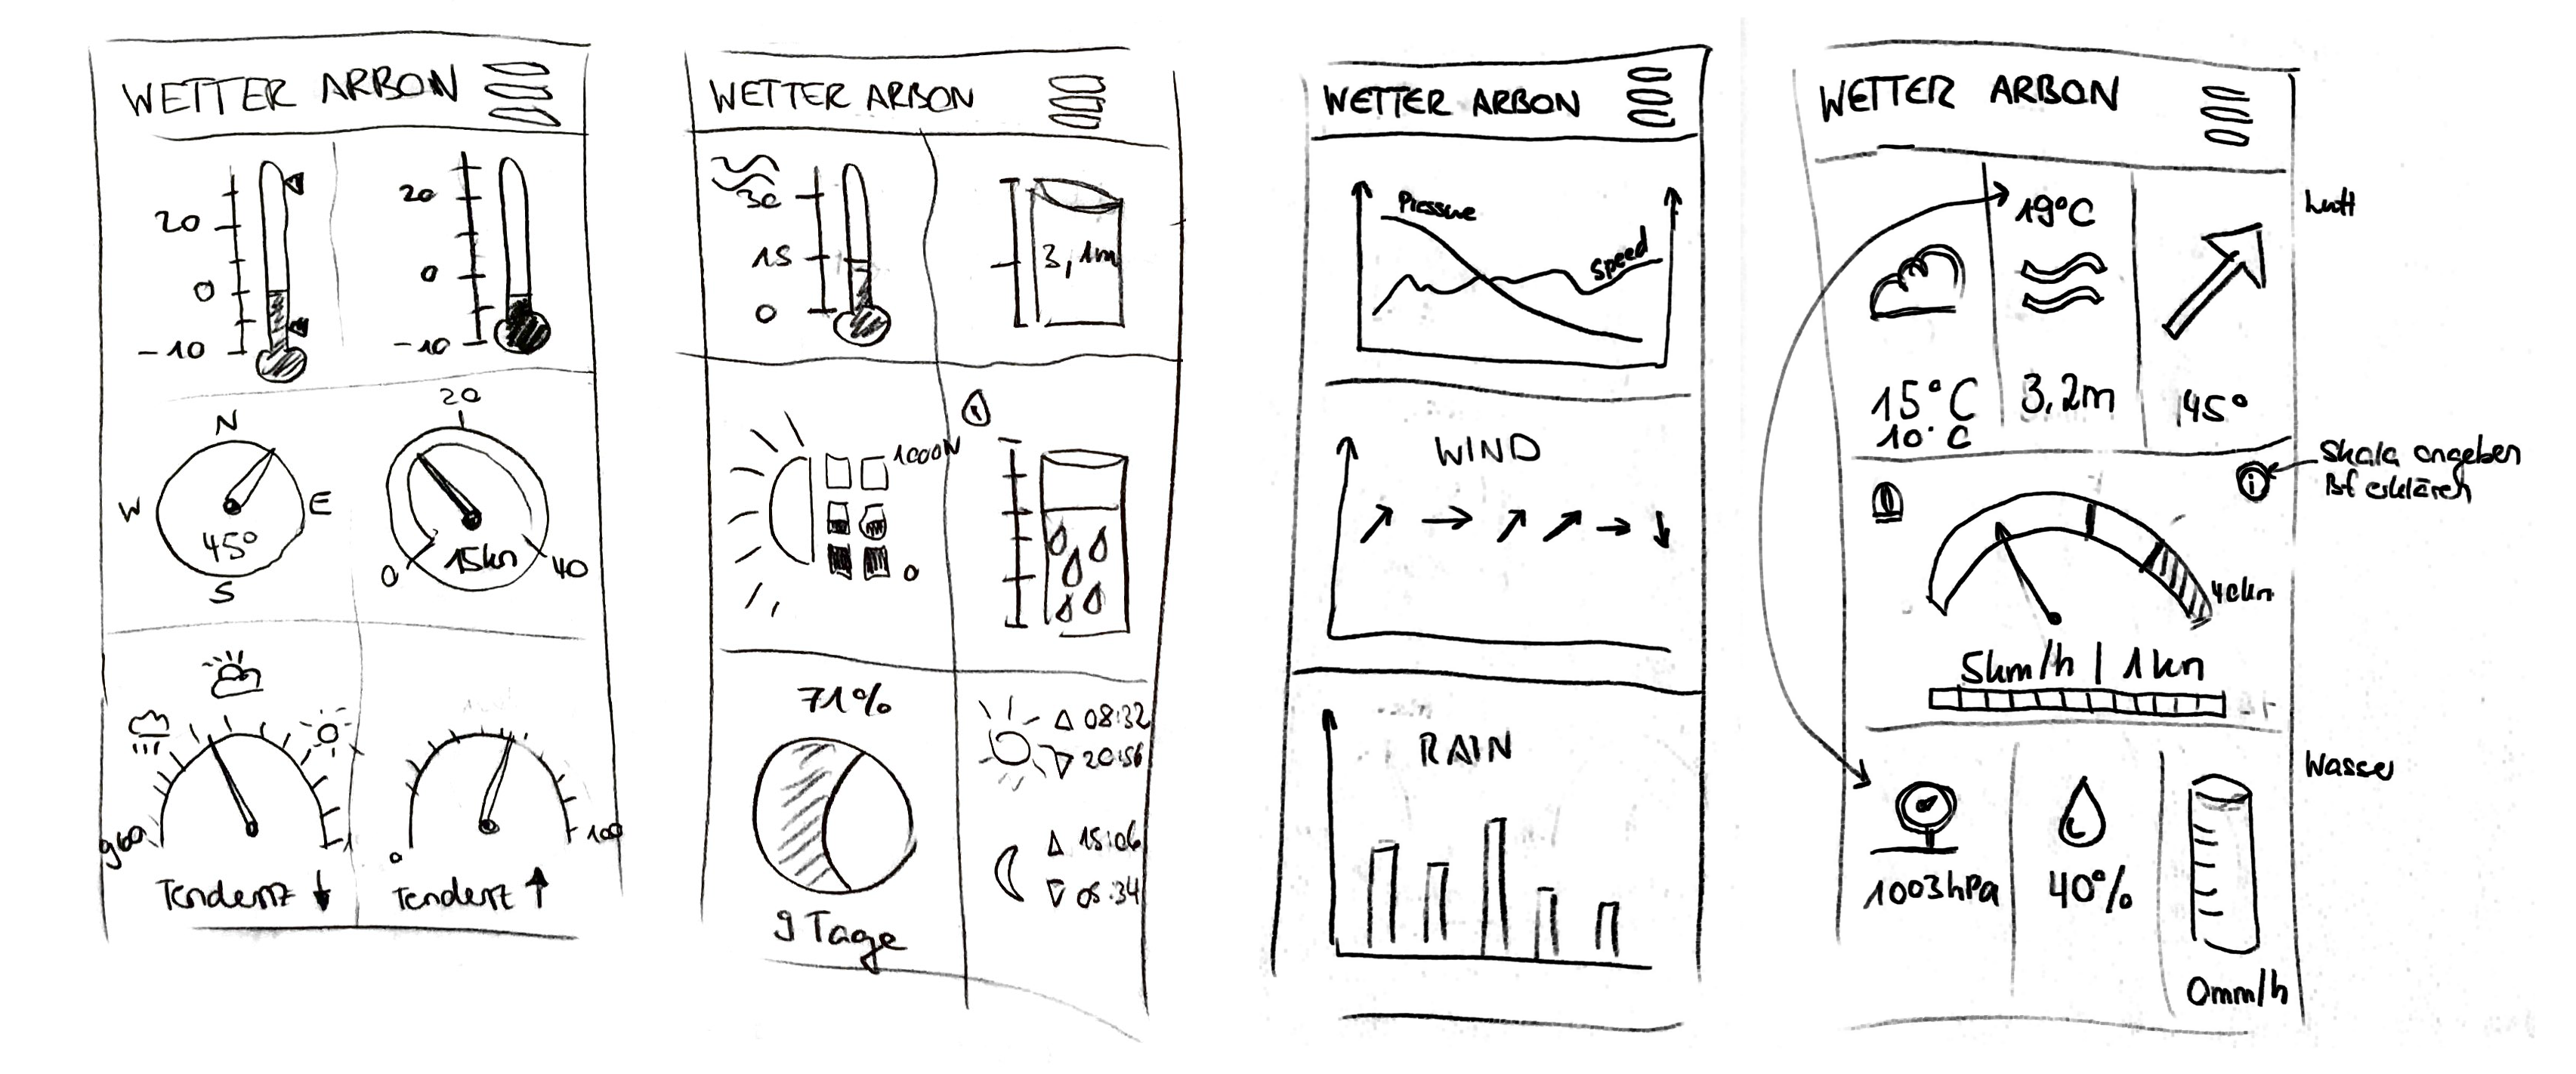
\includegraphics[width=\textwidth-2\fboxsep-2\fboxrule]{img/scribbles}}
	\centering
	\caption{Erste Designentwürfe nach dem Mobile First Prinzip}
	\label{img:scribbles}
\end{figure}

Beim Erstellen der ersten Designentwürfe, wie in Abbildung \ref{img:scribbles}, dargestellt, stellte sich schnell heraus, dass die einfachste Möglichkeit die Daten auf allen Bildschirmgrössen darzustellenzu können, darin besteht, die Informationen in kleine logische Blöcke zu unterteilen. Diese Blöcke können dann verschieden angeordnet werden. Dieses Kachel-Design ist eine gängiges Prinzip um das Gestaltungsgesetz der Zusammengehörigkeit umzusetzen und eignet sich hervorradend im Zusammenhang mit dem Grid-Konezpt des responsive Designs, welches im Abschnitt \ref{subsec:responsiveFactors} erläutert wird.


\subsubsection{W3.css als Layout-Framework}
Sämtliche Artefakte unserer Arbeit sollen möglichst einfach gehalten werden. Für die Gestaltung der Benutzeroberfläche haben wir uns deshalb entschlossen ein CSS-Framework zu benutzen. Dieses soll möglichst einfach und intuitiv zu bedienen sein, das Kachel-Design (auch Card-Design genannt) unterstützen, eine ausführliche Dokumentation aufweisen und eine geringe Dateigrösse haben. Wir haben drei verschieden CSS-Frameworks evaluiert und bewertet. Das Resultat ist in Tabelle  \ref{table:css-framework} ersichtlich.

\begin{table}[htb!]
\setlength\extrarowheight{3pt} % for a more "open" look
\begin{tabularx}{\textwidth}{|>{\RaggedRight\hspace{0pt}}p{4cm}||X|X|X|}

\hline
& \bfseries\large \href{https://www.w3schools.com/w3css/default.asp}{W3.css}
& \bfseries\large \href{https://purecss.io/start/}{Pure.css}
& \bfseries\large \href{http://getbootstrap.com/docs/4.1/getting-started/introduction/}{Bootstrap}\\

\hline
\textbf{Grid Design}
& ++
& ++
& ++ \\

\hline
\textbf{Footprint}
& 23 kB
& 14 kB
& 141 kB \\

\hline
\textbf{Usability}
& ++
& +
& + \\

\hline
\textbf{Card-Design}
& +
& -
& ++ \\

\hline
\textbf{Dokumentation}
& +++
& 0
& ++ \\

\hline
\textbf{Cross-Browser}
& ++
& ++
& +++ \\

\hline
\textbf{Funktionsumfang}
& +
& 0
& ++ \\

\hline
\end{tabularx}
\caption{Beurteilungsmatrix der evaluierten css-Frameworks}
\label{table:css-framework} % label muss NACH caption stehen!!!!
\end{table}

\noindent
Als Sieger stellt sich das W3.css-Framework heraus, da es den besten Kompromiss zwischen Dateigrösse und Funktionsumfang bietet. Zumdem weist es eine hervorragende Dokumentation auf.


\subsubsection{Responsive Design}
\label{subsec:responsiveFactors}
Die Benutzeroberfläche muss Cross-Plattform-fähig sein d.h. die Darstellung muss sich je nach Bildschirmgrösse automatisch anpassen. Man nennt dies \textit{Responsive Design}. Die Idee des Responsive Web Design wurde 2010 von Ethan Marcotte in einem Artikel\footnote{ \url{http://alistapart.com/article/responsive-web-design}} des Magazins \textit{A List Apart} veröffentlicht. Hintergrund war, dass man nicht für jedes neue Gerät eine eigene Webseite erstellen wollte. Marcotte schreibt von drei Faktoren, die ein responsive Design benötigt: Fluid grids, flexible images und media queries. Fluid grids bedeutet, dass sich die Anordnung der Elemente dynamisch der Bildschirmgrösse anpasst. Flexible Bilder haben keine feste Grösse sondern nutzen den ihnen zu Verfügung stehenden Platz optimal aus und die Media queries sind die technische Basis für die beiden oberen Anforderungen.

\begin{figure}[h!]
  \fbox{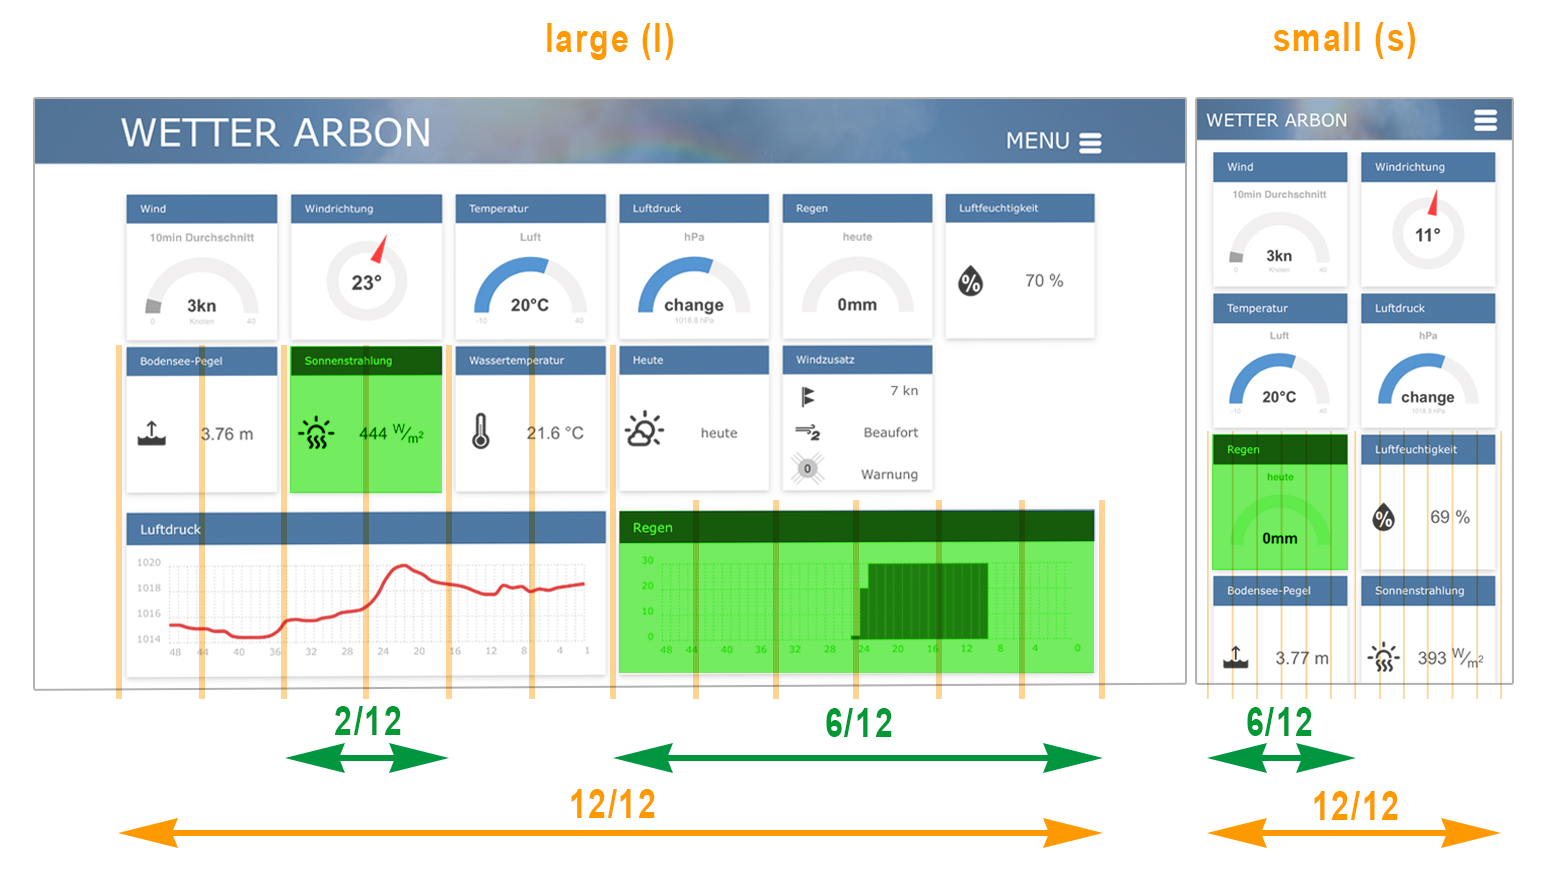
\includegraphics[width=\textwidth-2\fboxsep-2\fboxrule]{img/kacheln2}}
	\centering
	\caption{Anordnung der Kacheln auf grossen und kleinen Bildschirmen}
	\label{img:kacheln2}
\end{figure}

\noindent
Das Konezt des Grid-View teilt den Bildschirm bzw. den zur Verfügung stehnden Platz unabhängig von dessen Grösse in zwölf Spalten ein (siehe orange Markierung in Abbildung\,\ref{img:kacheln2}). Über eine media-Query fragt die Webseite die Grösse des Bildschirms in Pixel ab und bestimmt dann wieviele Spalten breit ein Element sein soll (grüne Markierung in Abbildung\,\ref{img:kacheln2}). Die gleiche Kachel ist also auf einem grossen Bildschirm  \nicefrac{2}{12} breit und auf einem kleinen Bildschirm \nicefrac{6}{12}. Unter \emph{w3.css} sind drei Bildschirmgrössen vorgesehen (small, medium und large). Die Grenzen sind folgendermassen festgelegt:

\begin{itemize}
\item Small: s $\leq$ 600px (z.B. iPhone Hochformat)
\item Medium: 600px < m $\leq$ 992px (z.B. iPhone Querformat, iPad Hochformat)
\item Large: 992px < l (z.B. Desktop)
\end{itemize}

\noindent
Den Kacheln kann nun über die Klasse (z.B. l2 m3 s6) deren Verhalten bei den drei Bildschirmgrössen vorgeschrieben werden. Die Kacheln mit den aktuellen Wetterdaten sind zum Beispiel auf grossen (large) Bildschirmen \nicefrac{2}{12}, auf mittleren Bildschirmen \nicefrac{3}{12} und auf kleinen Bildschirmen \nicefrac{6}{12} breit. Bei der Darstellung der Wetterdatenverläufe werden bei mittleren und grossen Bildschirmen zwei nebeneinander dargestellt (\nicefrac{6}{12}) und bei kleinen Bildschirmen alle untereinander (\nicefrac{12}{12} ), wie in Listing\,\ref{lst:kacheln} ersichtlich.

\vspace{3mm}
\begin{lstlisting}[label=lst:kacheln,caption=Konfiguration der Anzahl Kacheln abhähngig von der Bildschirmgrösse, language=HTML5, style=htmlcssjs]
<!-- Aktuelle Daten -->
<div class="l2 m3 s6">
	...
</div>

<!-- Datenverlauf -->
<div class="l6 m6 s12">
  ...
</div>
\end{lstlisting}
\vspace{3mm}

%% ############################################################################
%% Unterkapitel
%% ############################################################################
\subsection{Grafische Darstellung der aktuellen Wetterdaten}
Die Anzeigeelemente für die aktuellen Messwerte sollen ebenfalls mit Hilfe eines Frameworks erstellt werden. Damit die Grafiken optimal mit dem responsive Layout zusammenspielen, müssen sie ein flexibles Layout aufweisen d.h. ihre Grösse dem vorhanden Platz anpassen. Am Besten nicht nur beim Aufrufen der Seite, sondern auch beim Ändern der Fenstergrösse. Zudem muss es einfach möglich sein die Werte zu aktualisieren.

Die Anzeige sollte möglichst ein klares Design aufweisen aber trotzdem individuell anpassbar sein. Ein sehr einfaches JavaScript-Framework ist \textit{JustGage}\footnote{ \url{http://justgage.com}}. Die Grafiken lassen sich über eine JavaScript-Datei konfigurieren, die Grafiken selbst sind im svg-Format und somit von praktisch allen Browsern darstellbar. JustGage basiert auf der \textit{Raphaël}\footnote{ \url{http://dmitrybaranovskiy.github.io/raphael/}}—JavaScript Bibliothek.

\begin{figure}[h!]
  \fbox{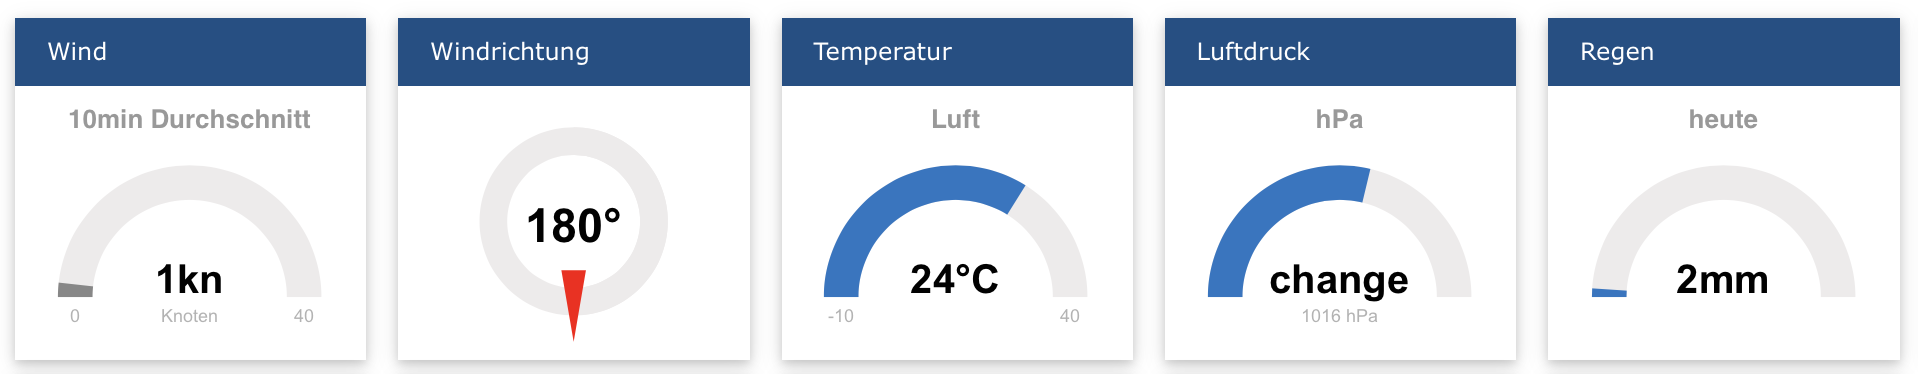
\includegraphics[width=\textwidth-2\fboxsep-2\fboxrule]{img/gauges}}
	\centering
	\caption{Anzeigelemente mit Justgage/Raphaël}
	\label{img:gauges}
\end{figure}

Raphaël ist eine kleine JavaScript-Bibliothek, die Ihnen die Arbeit mit Vektorgrafiken im Web erleichtern soll. Wenn Sie z.B. Ihr eigenes Diagramm oder Bildausschnitt erstellen und das Widget drehen möchten, können Sie dies einfach und bequem mit dieser Bibliothek erreichen. Raphaël verwendet die SVG W3C Recommendation und VML als Grundlage für die Erstellung von Grafiken. Dies bedeutet, dass jedes grafische Objekt, das Sie erstellen, auch ein DOM-Objekt ist, so dass Sie JavaScript-Ereignisbehandler anhängen oder später ändern können. Raphaëls Ziel ist es, einen Adapter zur Verfügung zu stellen, der das Zeichnen von Vektorgrafiken browserübergreifend und einfach macht.


\begin{lstlisting}[label=lst:gaugeJS,caption=Konfiguration der Gauge, language=JavaScript,mathescape, style=htmlcssjs]
var temperature_gauge = new JustGage({
  id:     temperature_gauge,
  value:  initialValues.v1.data.temperature.value,
  min:    -10,
  max:    40,
  symbol: C,
  title:  Luft
});
\end{lstlisting}

Um die Grafik anzuzeigen muss nur ein DIV mit der selben ID auf der Webseite erstellt werden wie in Listing \ref{lst:gaugeHTML} dargestellt.

\begin{lstlisting}[label=lst:gaugeHTML,caption=Container für die SVG-Grafik (Gauge), language=HTML5, style=htmlcssjs]
<!-- Lufttemperatur -->
<div class="w3-cell w3-col l2 m3 s6">
  <div class="w3-card">
    <div class="w3-container">
      <p>Temperatur</p>
    </div>
    <div id="temperature_gauge" class="gauge"></div>
  </div>
</div>
\end{lstlisting}

Die Messwerte sind einerseits über den Titel beschrieben, sie enthalten aber zusätzlich ein passendes Icons. Es wurde eine Icon-Bibliothek gewählt, die möglichst alle benötigen Icons enthält, die kostenlos ist, und deren Grafiken im svg-Format vorliegen. Als geeignet schienen die \textit{Weahter Icons}\footnote{\url{http://erikflowers.github.io/weather-icons/}} von Erik Flowers.


\begin{figure}[h!]
  \fbox{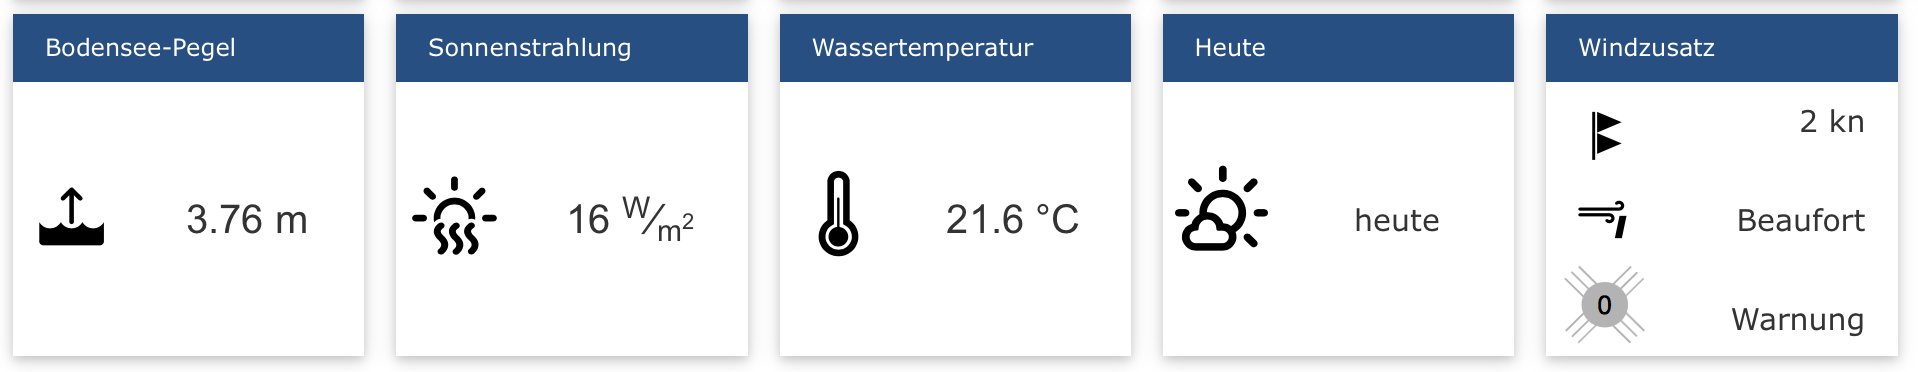
\includegraphics[width=\textwidth-2\fboxsep-2\fboxrule]{img/icons}}
	\centering
	\caption{Icons aus der Weather Icons Bibliothek}
	\label{img:icons}
\end{figure}





%% ############################################################################
%% Unterkapitel
%% ############################################################################
\subsection{Grafische Darstellung der Wetterdatenverläufe}
Die Wetterverlaufsdarstellung soll einen Überblick über die Wettertendenz der letzten beiden Tage liefern. Die Samplerate beträgt 1h, d.h. die Daten werden aus der Tabelle der historischen Werte abgerufen.

\begin{figure}[h!]
  \fbox{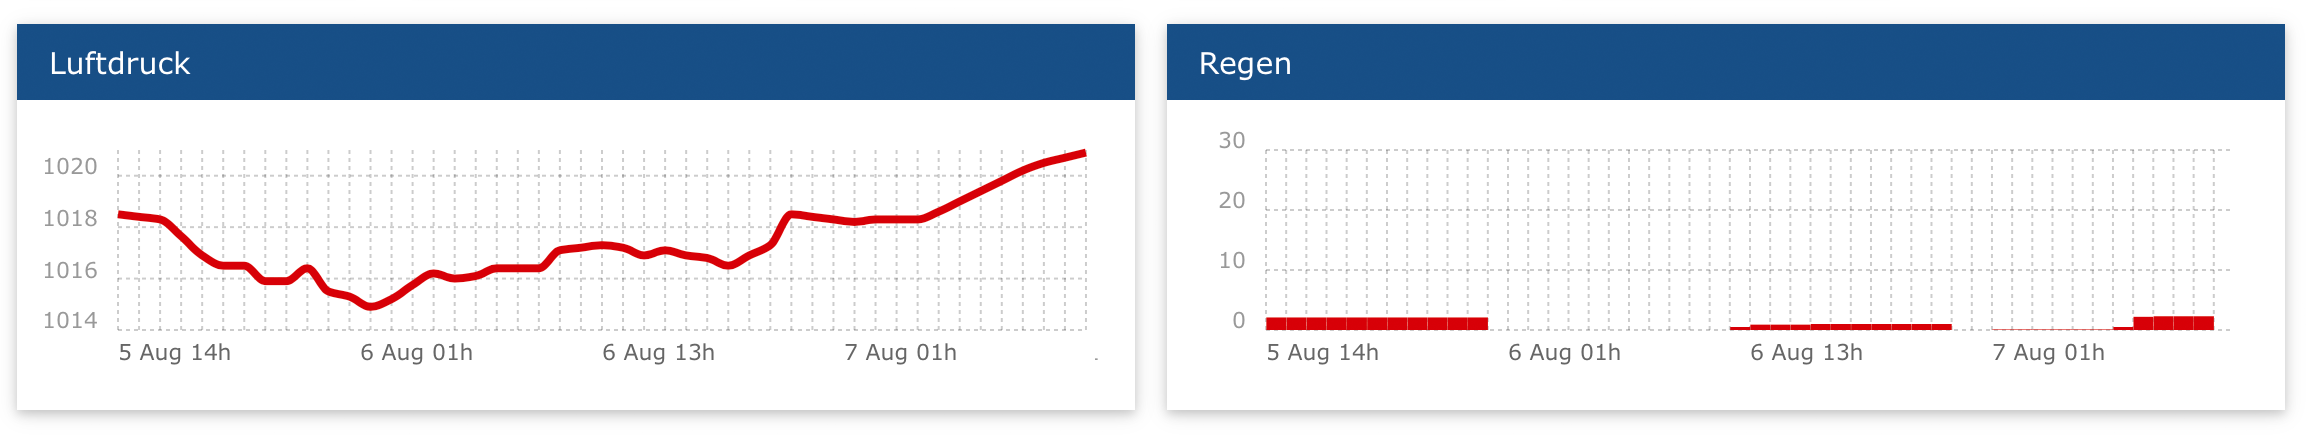
\includegraphics[width=\textwidth-2\fboxsep-2\fboxrule]{img/charts}}
	\centering
	\caption{Verlaufsdiagramm mit chartist.js}
	\label{img:charts}
\end{figure}



\subsubsection{Auswahl des JS-Frameworks}
Für die Darstellung der Messwertverläufe soll ebenfalls auf eine Bibliothek zurückgegriffen werden. Als erstes wurden js-Bibliotheken gesucht, die ein ansprechendes Design aufweisen. Übrig geblieben sind die in Tabelle \ref{table:js-framework} aufgeführten drei js-Bibliotheken. Diese wurden auf ihre Eignung geprüft. Zwingend mussten die Grafiken im SVG-Dateiformat vorliegen, sodass die Cross-Browser-Kompatiblität und das responsive Verhalten sichergestellt ist. Die Daten sollten zudem als JSON übergeben werden können. D3 ist zwar DIE js-Bibliothek wenn es um Visualisierungen im Web geht, hat aber keine vorgefertigten Diagramme und benötigt entsprechend viel Aufwand und Einarbeitungszeit, was wir explizit nicht möchten.

\begin{table}[htb!]
\setlength\extrarowheight{3pt} % for a more "open" look
\begin{tabularx}{\textwidth}{|>{\RaggedRight\hspace{0pt}}p{3.5cm}||X|X|X|}

\hline
& \bfseries\large \href{https://gionkunz.github.io/chartist-js/index.html}{chartist.js}
& \bfseries\large \href{https://www.fusioncharts.com}{Fusion Charts}
& \bfseries\large \href{https://developers.google.com/chart/}{Google Charts}\\

\hline
\textbf{Footprint}
& 10 kB
& >1000 kB
& 110 kB \\

\hline
\textbf{Barrierefrei}
& +
& 0
& + \\

\hline
\textbf{Anpassbarkeit}
& ++
& +++
& ++ \\

\hline
\textbf{Dokumentation}
& +++
& +++
& ++ \\

\hline
\textbf{Kostenlos}
& +
& --
& + \\

\hline
\textbf{Funktionsumfang}
& ++
& +++
& + \\

\hline
\end{tabularx}
\caption{Beurteilungsmatrix der evaluierten js-Frameworks}
\label{table:js-framework} % label muss NACH caption stehen!!!!
\end{table}

\noindent
Chartist.js stellte den besten Kompromiss zwischen Funktionsumfang, Einfachheit und Dokumentation dar. Insbesondere die Dateigrösse war ausschlaggebend, da die Webseite, wie in Abschnitt \ref{subsec:googleAnalytics} erklärt, primär von mobilen Nutzer genutz wird.

% Code-Beispiel
\begin{lstlisting}[label=lst:charts,caption=Konfiguration der Verlaufsdiagramme, language=HTML5, style=htmlcssjs]
//Luftdruck
var Barometer = {
  labels: [48,...,1],
  series: [dataBarometerHistoric]
};
new Chartist.Line('#air-chart', Barometer);

//Regen
var Rain = {
	labels: [48,...,1],
	series: [dataRainHistoric]
};
var options = {
low: 0,
high: 30,
};
new Chartist.Bar('#rain-chart', Rain, options);
\end{lstlisting}
\ \\


Zur Verlaufsdarstellung wird primär das Linien- und Balkendiagramm verwendet, wie in Abbildung \ref{img:charts} aufgezeigt. Für jede Grafik wurde entschieden ob eine automatische Y-Achs-Skalierung sinnvoll ist oder nicht. Bei der Windgeschwindigkeit und beim Pegel wurd bewusst eine fixe Skalierung verwendet, damit auf den ersten Blick klar ist, ob der Wert eher hoch oder eher tief ist. Beim Luftdruck hingegen ist die Tendenz wichtig, weshalb möchglichst die gesamte Höhe des Diagramms genutzer werden soll. Es wird daher eine automaitsche Y-Achs-Skalierung verwendet. Die Konfiguration erfolgt in einem einfach JS-File wie in Listing Listing \ref{lst:charts}  dargestellt. Unter \textit{options} kann die y-Achse auf die gewünschten Werte fixiert werden.\newline


\subsubsection{Anzeige der Windrichtung}
Die Anzeige des Windrichtungsverlaufs ist nicht ganz trivial da sie von 0 bis 360 Grad geht und ohne Unterbruch wieder zu 0 Grad. In der Praxis wird dazu häufig die Darstellung von Pfeilen verwendet wie in Abbildung \ref{img:windrichtung}, links dargestellt. Es konnt jedoch kein Framework gefunden werden, das diese Darstellungsart als Template zur Verfügung stellt. Die Anzeige der Windrichtung wird deshalb über ein Punktdiagramm, wie in Abbildung \ref{img:windrichtung}, rechts dargestellt verwendet.

\begin{figure}[h!]
	\centering
  \fbox{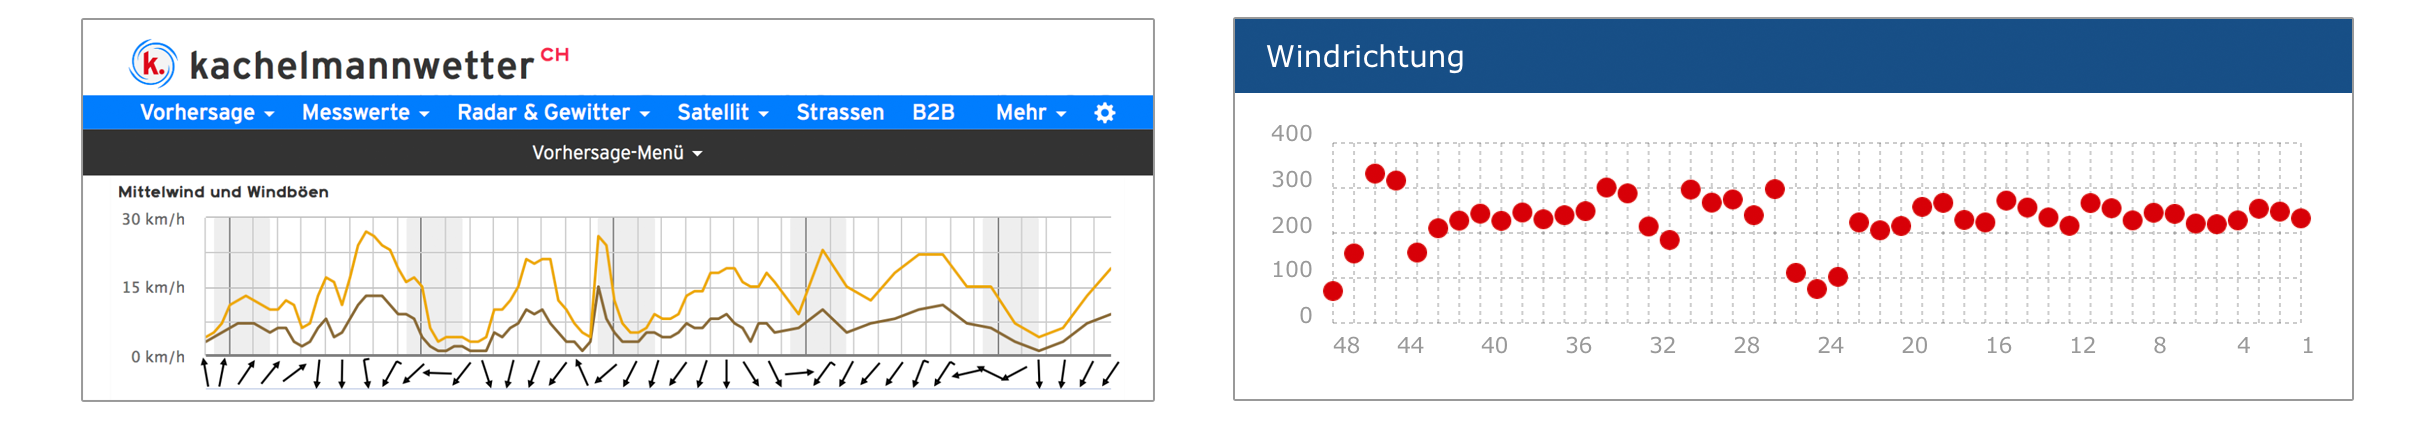
\includegraphics[width=\textwidth-2\fboxsep-2\fboxrule]{img/windrichtung}}
	\caption{Windrichtungsanzeige soll und ist}
	\label{img:windrichtung}
\end{figure}

\subsubsection{Vergleich Prognose/Ist Windgeschwindigkeit}
Insbesondere bei Seglern sind Windprognosenseiten sehr beliebt. Sie liefern Windprognosen bis zu fünf Tage voraus. Bei allen Vorhersagediensten ist nicht erkennbar wie gut dir Prognose war. Geanu dies ist aber eine spannende Frage weshalb dieser Vergleich auf der Webseite angezeigt werden soll. Die Messdaten der Wetterstation werden daher mit zwei kostenlosen Vorhersagediensten verglichen. Dabei wird jeweils die Dreitagesvorschau betrachtet. Für die Windvorhersage wurden folgende zwei Anbieter ausgewählt:

\begin{itemize}
\item Openweathermap
\item Windfinder
\end{itemize}

\noindent
Opeanwathermap ist einer der wenigen Anbieter, der eine kostenlose API zur Verfügung stellt. Windfinder ist unter den Seglern das beliebteste Tool. Die Vorhersagedaten werden von den Anbietern nur in die Zukunft angezeigt d.h. wie die Vorhersage von gestern war ist nicht mehr ersichtlich. Aus diesem Grund müssen die Vorhersagedaten abgegriffen und gespeichert werden. Für den Prognoseanbieter haben wir uns für Openweathermap und windfinder entschieden. OWM bietet eine kostenlose Web-API. Windfinder ist eines der beliebtesten Seglertools, bietet aber keine API sondern lediglich ein Widget für den gewünschten Standort an. Dies Daten müssen somit aus dem Windfinder-Widget, siehe Abbildung \ref{img:windfinder}, mittels Crawler extrahiert werden, analog Listing \ref{lst:kttgCrawler}.

\begin{figure}[h!]
	\centering
  \fbox{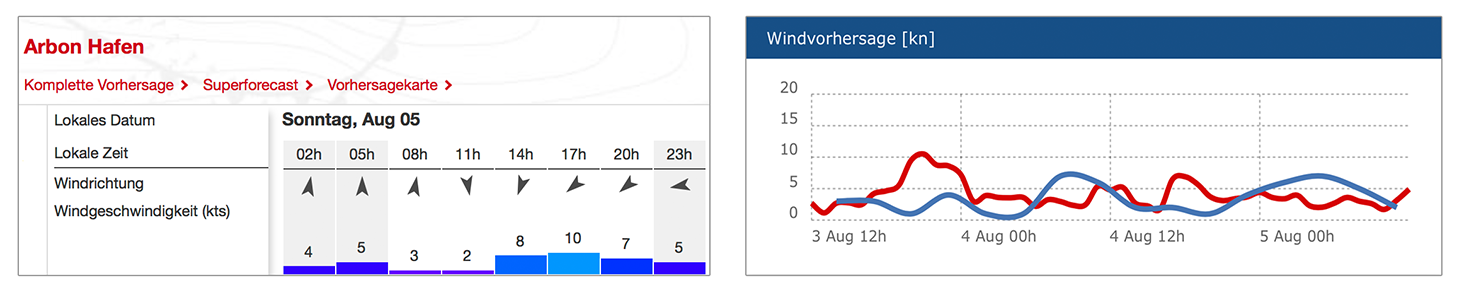
\includegraphics[width=\textwidth-2\fboxsep-2\fboxrule]{img/windfinder}}
	\caption{Widget von Windfinder}
	\label{img:windfinder}
\end{figure}

Nach den ersten Auswertungen wurde festgestellt, dass die Wettervorhersagedaten von Openweathermap absolut unbrauchbar waren. Sie lagen permanent zwischen 0 und 1 Knoten auch wenn die Wetterstation 15 Knoten messte. Die Vorhersage von Openweathermap wurde deshalb nicht mehr weitervervolgt.

Die Abfrage der Datenban stellt sich als recht kompliziert heraus. Sodass entschieden wurde eine VIEW einzusetzten. Diese wird dynamisch bei Aufrufen erzeugt und enthält die gewünschten Daten. Der SQL-Befehl für die Erzeugung der VIEW ist vereinfacht in Listing \ref{lst:viewForecast} aufgeführt. Primär gibt es zwei Bediungungen. Erstens sollen nur die Dreitageverhersagewerte verwendet werden und zweitens sollen die Vorhersagewerte verwendet werden, die am nächsten bei der aktuellen Zeit liegen. Da das Vorhersageintervall 3 Stunden beträgt ist die Verhersage maximal 1.5 Stunden verschoben.

%View erstellen
\begin{lstlisting}[label=lst:viewForecast,caption=Erzeugung der VIEW für den Forecast-Vergleich, language=SQL, style=htmlcssjs]
SELECT *
FROM 'tblcompwindfinder'
WHERE
(datetime + interval 3 day) <= now() #heute vor drei Tagen
AND
abs(timediff(datetime,now())) <= 13000) #innerhalb +/- 1.5h
ORDER BY datetime DESC
LIMIT 3
\end{lstlisting}

%\Diskussionspunkt{- Eintagesvorschau}\newline
%\Diskussionspunkt{- Mittels Tableau? Eigen Webseite?}\newline
%\Diskussionspunkt{- Bild mit Vergleich von Messwerten, Vorhersage Windfinder und Vorhersage Openweathermap}\newline

% Graphen, der den heutigen Tag, links davon die letzten 14 Tage und rechts davon die nächsten drei Tage anzeigt.
% Pro Anbieter und Prognoseart (1Tag bzw. 3 Tage) wird ein eigener Graph erstellt.
% Aus diesen Gründen wird die Webseite zwar veröffentlicht, aber kein Link dazu auf der Webseite zur Verfügung gestellt.
% Werte aus der Stundenwert-Datenbank?

%% ############################################################################
%% Unterkapitel
%% ############################################################################
\subsection{Anzeige der aktuellen Sturmwarn-Situation}
\label{subsec:sturmwarnung}

% was ist der Sturmwarndienst und wie werden die verschiedenen Stufen dargestellt
Auf dem Bodensee gibt es einen Sturmwarndienst, der die Schiffsführer vor aufkommendem Sturm warnen soll. Der Sturmwarndienst wird vom Deutschen Wetterdienst in Zusammenarbeit mit MeteoSchweiz betrieben. Rund um den Bodensee sind dafür über 60 Sturmwarnleuchten installiert (Abbildung \ref{img:sturm2}). Es wird unterschieden zwischen \textit{Starkwindwarnung} und \textit{Sturmwarnung}. Erstere weist auf auf starke Windböen zwischen 25 Knoten und 33 Knoten hin und wird durch Aufleuchten von orangefarbigen Blinklichtern mit ca. 40 orangefarbigen Blitzen pro Minute an den Sturmwarnleuchten signalisiert. Letzere kündigt das Auftreten von Windböen von 34 Knoten und mehr an und wird durch Aufleuchten von orangefarbigen Blinklichtern mit ca. 90 orangefarbigen Blitzen pro Minute an den Sturmwarnleuchten signalisiert (gemäss Anlage B der Bodensee-Schifffahrts-Ordnung\footnote{ \url{https://www.admin.ch/opc/de/classified-compilation/19760005/index.html}}, BSO).

\begin{figure}[htbp!]
	\centering
  \fbox{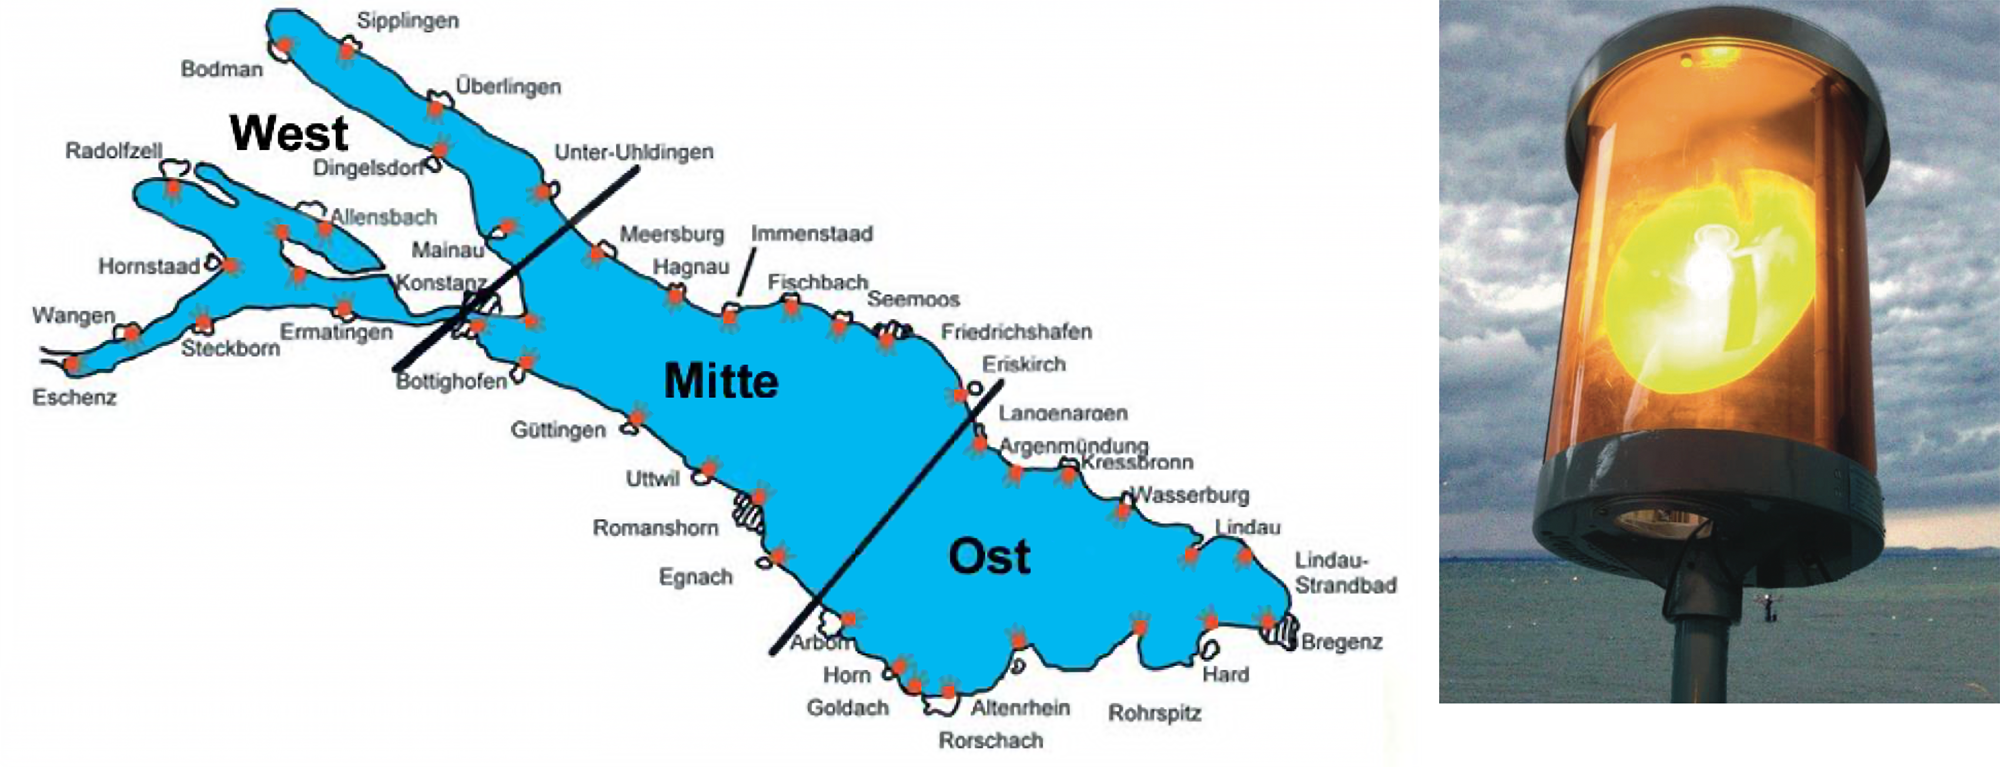
\includegraphics[width=\textwidth-2\fboxsep-2\fboxrule]{img/sturm2}}
	\caption{Warleuchten des Sturmwarndiensts auf dem Bodensee}
	\label{img:sturm2}
\end{figure}



\subsubsection{Eingeschränkte Bezugsquellen}
% Problem: Kostenpflichtige Informaiton
Den aktuellen Status der Sturmwarnung kann sowohl beim Deutschen Wetterdienst, als auch bei Meteoschweiz kostenpflichtig bezogen werden (ca. 1300CHF/Jahr). Als kostenlose Alternative gibt es nur zwei browserkomatible Quellen: Das eine ist die Warnseite\footnote{ \url{https://www.meteoschweiz.admin.ch/home.html?tab=alarm}}  von Meteoschweiz und das andere die Anzeige auf der Webseite\footnote{ \url{http://www.kttg.ch/kapo/htm/stwarn.shtml}} der Kantonspolizei Thurgau, siehe Abbildung \ref{img:sturmZeit}, links. Eine kostenlose API steht ebenfalls nicht zur Verfügung. Meteoschweiz verbietet es zudem, Informaitonen von ihrer Website abzugreifen. Wir haben deshalb beim Amt für Informatik des Kantons Thurgau, welches die Seite der Kantonspolizei betreut, die Erlaubnis eingeholt, die Sturmwarndaten ihrer Webseite abgreifen zu dürfen. Beim Vergleich der verschiedenen Quellen wurde festgestellt, dass die Warnleuchten jeweils mit einigen Minuten Verspätung gegenüber der Meldung von Meteoschweiz eingeschaltet werden, siehe Abbildung \ref{img:sturmZeit}. Da der Verzug nicht konstant ist, muss davon ausgegangen werden, dass die Warnleuchten manuell eingeschaltet werden.\\
\Diskussionspunkt{Verweis auf E-Mail im Anhang}\\

\begin{figure}[h!]
	\centering
  \fbox{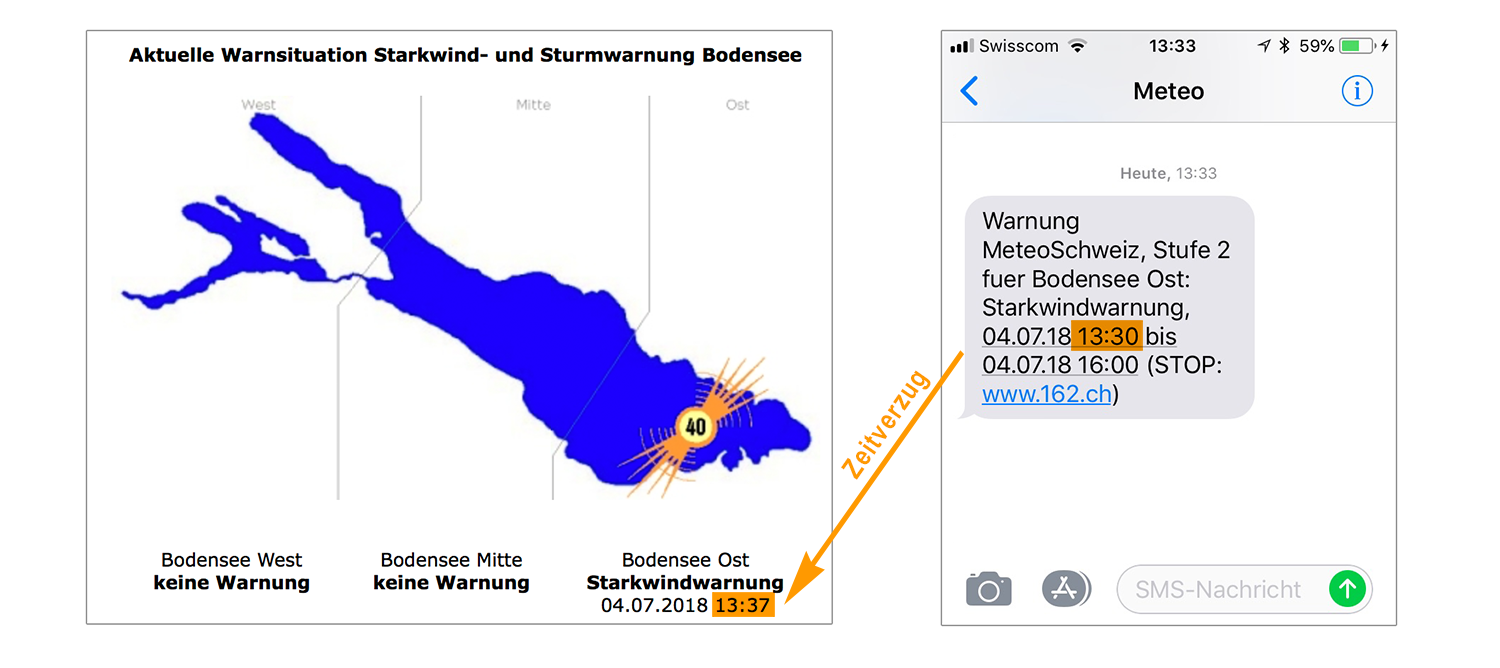
\includegraphics[width=\textwidth-2\fboxsep-2\fboxrule]{img/sturmZeit}}
	\caption[Zeitverzug zwischen Sturmwarnmeldung und Anzeige]{Zeitverzug zwischen der Warnmeldung von Meteoschweiz und dem Einschalten der Warnleuchten durch die Kantonale Notrufzentrale (KNZ) in Frauenfeld}
	\label{img:sturmZeit}
\end{figure}


\subsubsection{Abgreifen der Sturmwarndaten} % screen scrapping
% Problem 1: keine API -> wenn Seite ändert, muss Crawler angepasst werden.
Die Sturmwarndaten werden periodisch mittels Python-Skript ausgelesen. Als Web-Scrapper kommt die Python-Bibliothek \href{https://www.crummy.com/software/BeautifulSoup/}{\emph{BeautifulSoup}} zum Einsatz. Das Auslesen von Webseiten wird auch \emph{web scraping} genannt. Die Idee dahinter ist, die gewünschte Information auf Grund ihrer Element-Bezeichnung (\texttt{<td>}), ihres Attributs (\texttt{class="titelfett"}) oder Hierarchistufe (\texttt{tr:nth-of-type(4)}) eindeutig zu identifizieren. Um diese eindeutige Identifikation herauszufinden wurde das Google Chrome-Plugin \href{https://selectorgadget.com/}{\emph{SelectorGadget }} verwendet. Listing \ref{lst:kttgCrawler} zeigt die gesamte Abfrage. Darin ist das Problem dieser Methode gut erkennbar. Ändert die URL oder die Bezeichung bzw. Struktur der Seite, liefert das Skript nicht mehr die gewünschten Daten. Da das Web-Scrapping jedoch die einzige kostenlose Möglichkeit darstellt um die Daten zu erhalten, muss dieses Risiko akezptiert werden.


\begin{lstlisting}[label=lst:kttgCrawler,caption=Web-Scrapper für die Sturmwarndaten, language=python, style=py]
page = requests.get('http://www.kttg.ch/kapo/htm/stwarn.shtml')
soup = BeautifulSoup(page.text, 'html.parser')

# Einschaltzeit auslesen
soup.select('table tr:nth-of-type(4) td'):

# Status auslesen
soup.select('.titelfett strong'):
\end{lstlisting}




\subsubsection{Eigener Sturmwarndienst mit Hilfe der Messwerte}
% Problem 2: Öffnungszeiten -> keine Warnung in der Nacht
Der Sturmwarndienst wie in Abschnitt \ref{subsec:sturmwarnung} beschrieben, ist kein 24h-Service. Der Dienst ist nur tagsüber aktiv zu den aufgelisteten Warnzeiten\footnote{ \url{https://kapo.tg.ch/public/upload/assets/56408/A5\%20Sturmwarnung.pdf}}, was aus Sicht der Sicherheit auf dem See nicht sehr sinnvoll ist.

\begin{itemize}
\item 1. April - 31. Oktober: 06:00 - 22:00 Uhr
\item 1. November - 31. März: 07:00 - 20:00 Uhr
\end{itemize}

\noindent
% Problem 3: rechtliche Verbindlichkeit der Sturmwarnung -> Zuverlässigkeit der anzeigen
Es liegt nahe auf Grund der eigenen Windmessdaten eine Sturmwarnung anzuzeigen bzw. einen Benachrichtungsservice, wie in Kapitel \ref{notifications} beschrieben, anzubieten. In der Bodensee-Schifffahrts-Ordnung (BSO) Art. 6.13, steht jedoch:

\begin{quote}
\flqq Bereits bei Starkwind- und Sturmwarnung muss der Schiffsführer die durch die Umstände gebotenen Massnahmen treffen.\frqq
\end{quote}

\noindent
 Die Sturmwarnung auf dem Bodensee gesetzlche Pflichten mit sich bringt, haben wir uns entschlossen nur die offiziellen Daten anzuzeigen und nicht anderweitige Sturmwarnungen. Meteoschweiz bietet zudem auf ihrer MeteoSchweiz-App\footnote{ \url{https://www.meteoschweiz.admin.ch/home/service-und-publikationen/beratung-und-service/meteoschweiz-app.html}} die Möglichkeit von Push-Nachrichten bei Windwarnungen.



%-> Meteoschweiz schickt in der Nacht keine SMS????? bzw. erstellt keine JSON????

% ins Kapitel API bzw. Cronjobs übernehmen
%Der Status der drei Teilabschnitte wird dann mintütlich in die Datenbank geschrieben. So kann der aktuelle Stand normal über die API abgefragt werden.

% nur im Vortrag erwähnen
% DAs JSON von Meteoschweiz kann leider nicht verwendet werden, da dessen URL bei jedem Update wechselt. Der genaue Pfad lässt sich nicht vorhersagen. Auf Grund des Zeitstempels lässt sich erahnen, dass es keine automatische Verbindung zwischen Meteoschweiz und den Sturmwarnleuchten am Bodensee gibt. Auf der Meteoschweiz-Seite ist z.B. der Zeitstempel 12:00 und auf der kttg.ch Seite 12:07. Wahrscheinlich erfolgt die Aktivierung manuell. Dies würde die Zeitdifferenz erklären.
% -> Foto Zeitstempel Meteoschweiz und kttg.ch
% Meteoschweiz leitet die Sturmwarnung an die Kantonspolizei Thurgau weiter. Diese schaltet die Sturmwarnung über eine eigne Software ein.


%% ############################################################################
%% Unterkapitel
%% ############################################################################
\subsection{Darstellung der historischen Daten}
Die Wetterstation misst sämtliche Messgrössen einmal pro Minute. Diese Minutenwerte werden einmal pro Stunde zusammengefasst und als historische Daten abgespeichert. Bereits bei der alten Wetterstation wurden Daten gespeichert. Zudem liegt ein Excel-File vor mit den Pegeldaten der letzten 50 Jahren, welche ebenfalls auf der Webseite verfügbar sein soll. Es gibt drei drei Grundlagen für die historischen Daten:

\begin{itemize}
\item Historische Daten der neuen Wetterstation
\item Historische Daten der alten Wetterstation
\item Excel mit Pegeldaten von 1953 bis 2005
\end{itemize}

Diese Daten und deren Anzeige auf der Webseite werden im Folgenden erläutert.



\subsubsection{Daten der neuen Wetterstation mit Tableau}\label{kap:Tableau}
Die historische Daten sollen möglichst interaktiv gestaltet sein und ein aussagekräftiges Bild des Wetterverhaltens aufzeigen. Die historischen Daten liegen als Stundenwerte in der Datebank vor.


Tableau Public \footnote{ \url{https://public.tableau.com/de-de/s/}} ist ein Visualisierungsprogramm, das die Möglichkeit bietet direkt auf die Datenbank zuzugreifen. Die Visualisierungen sind einfach zu erstellen und interaktiv vom Benutzer filterbar.
Tableu Public ist kostenlos mit der Einschränkung, dass sämtliche Visualisierungen öffentlich sind. In unserem Fall ist dies kein Problem, da wir die Visualisierungen sowieso veröffentlichen. Um Visualisierungen veröffentlichen zu können ist ein Account nötig. Die Visualisierung kann anschliessend in die eigene Webseite eingebettet werden.

Für die Auswertung haben wir uns auf die Lufttemperatur, die Windrichtung und -geschwindigkeit sowie den Regen konzentriert.
Der Vorteil von Tableau ist, dass die Visualisierungen sehr einfach angepasst werden können wenn z.B. neue Messdaten hinzukommen. Tableau bietet auch die Möglichkeit Darstellungen für verschiedene Display-Grössen anzulegen. Da der Benutzer selbst keine Eingaben machen kann, sondern nur Filter setzen, ist die Gefahr von SQL-Injektion nicht vorhanden.


Das Dashboard ist interaktiv d.h. der Benutzer kann den Betrachtungszeitraum selbst wählen. Die Grafiken passen sich automatisch der Auswahl an.
Wenn mit dem Mauszeiger über einen Messpunkt gefahren wird, werden zusätzliche Informaitonen angezeigt.


Hostpoint
Datenbankbenutzer -> IP eingeben (IP-Tool: http://ip.hostpoint.ch)
Anmeldedaten für tableau


\begin{figure}[h!]
	\centering
  \fbox{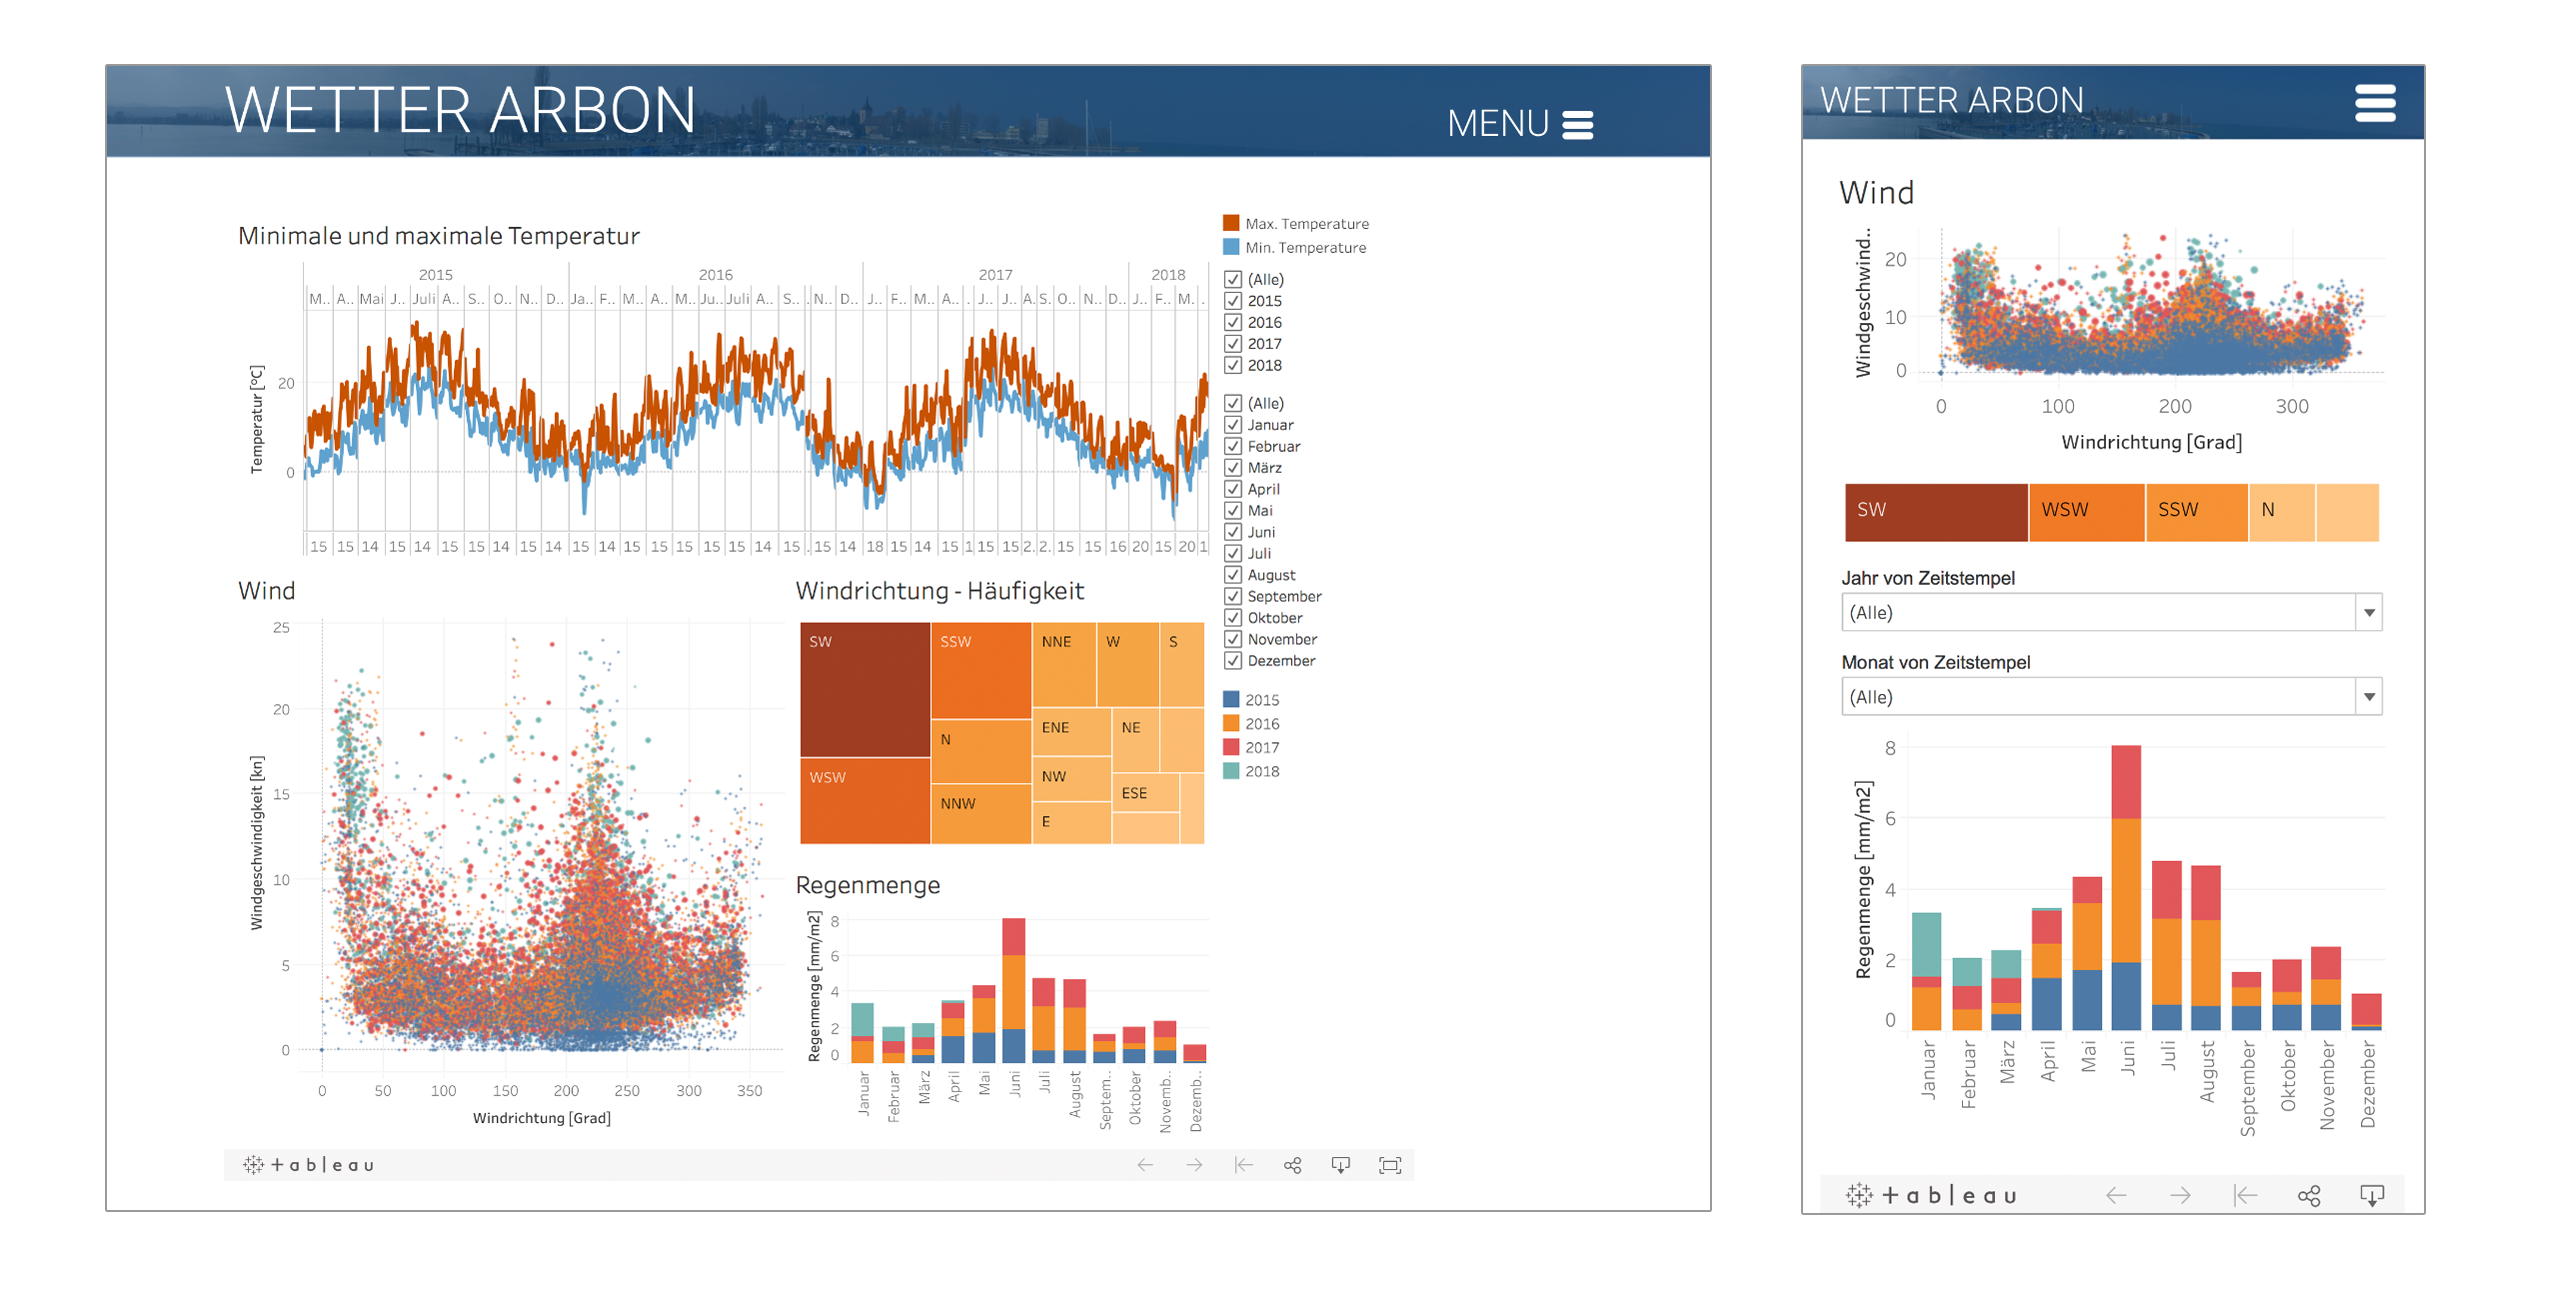
\includegraphics[width=\textwidth-2\fboxsep-2\fboxrule]{img/tableau}}
	\caption{Darstellung der historschen Daten (Desktop und Mobile)}
	\label{img:tableau}
\end{figure}


%Nachteil 2: Nicht responsive -> Workaround nötig
\noindent
Neben den vielen Vorteilen, hat Tableau Pubilc auf ein paar Nachteile. Das Dashbaord kann zwar frei gestaltet werden, ist aber nicht responsive d.h. es passt sich nicht der Bildschirmgrösse an. Das Problem wurd so gelöst, dass zwei verschiedene Dashboard (siehe Abbildung \ref{img:tableau}) erstellt werden. Eines für die Anzeige auf einem grossen Dispaly und eines für die Anzeige auf Mobiltelefonen. Beim Aufruf der Webseite wird die Bildschirmgrösse abgefragt und das entsprechende Dashboard geladen wie in Listing \ref{lst:histViewport} dargestellt.

\begin{lstlisting}[label=lst:histViewport,caption=Auswahl des Dashboards anahnd der Bildschirmgrösse, language=JavaScript, style=htmlcssjs]
(function () {
	var viewportWidth = $(window).width();
	if (viewportWidth > 767) {
		$('#area_3').load('application/php/tableauDesktop.php');
	}
	else {
		$('#area_3').load('application/php/tableauMobile.php');
	}
}());
\end{lstlisting}


% Nachteil 1: Keine direkte Verbindung zur Datenbank
\noindent
Ein weiteren Nachteil von Tableau Public, welches kostenlos ist gegenüber Tableau, welches kostenpflicht ist, ist dass Tableau Public keinen Live-Zugriff auf die Datenbank ermöglicht. Die Daten müssen somit manuell periodisch auf den Tableau Public Server kopiert werden, damit sie im Dashboard verfügbar sind.



\subsubsection{Daten der alten Wetterstation}
Abbildung \ref{img:histAlt} zeigt eine Zusammenfassung der von der alten Wetterstation vorhandenen Daten. Es gibt diverse Messlücken wie z.B. das komplette Jahr 2010 und 2012. Weiter sind z.T. unplausible Grössenordnungen vorhanden wie z.B. die Windgeschwindigkeit von 500, wo nicht klar ist, zu welcher Einheit dieser Angabe gehört. Die Wellenhöhe sieht mehr nach Signalrauschen aus, als nach plausiblem Messwert. Alles in allem sind in diesen Daten nicht viel nützliche Informationen vorhanden. Es wurde deshalb beschlossen auf der Webseite nur die historischen Daten der neuen Wetterstation anzuzeigen. Die Pegeldaten werden in die Grafik, wie in Abschnitt \ref{subsec:pegelhistory} beschrieben integriert.

\begin{figure}[h!]
	\centering
  \fbox{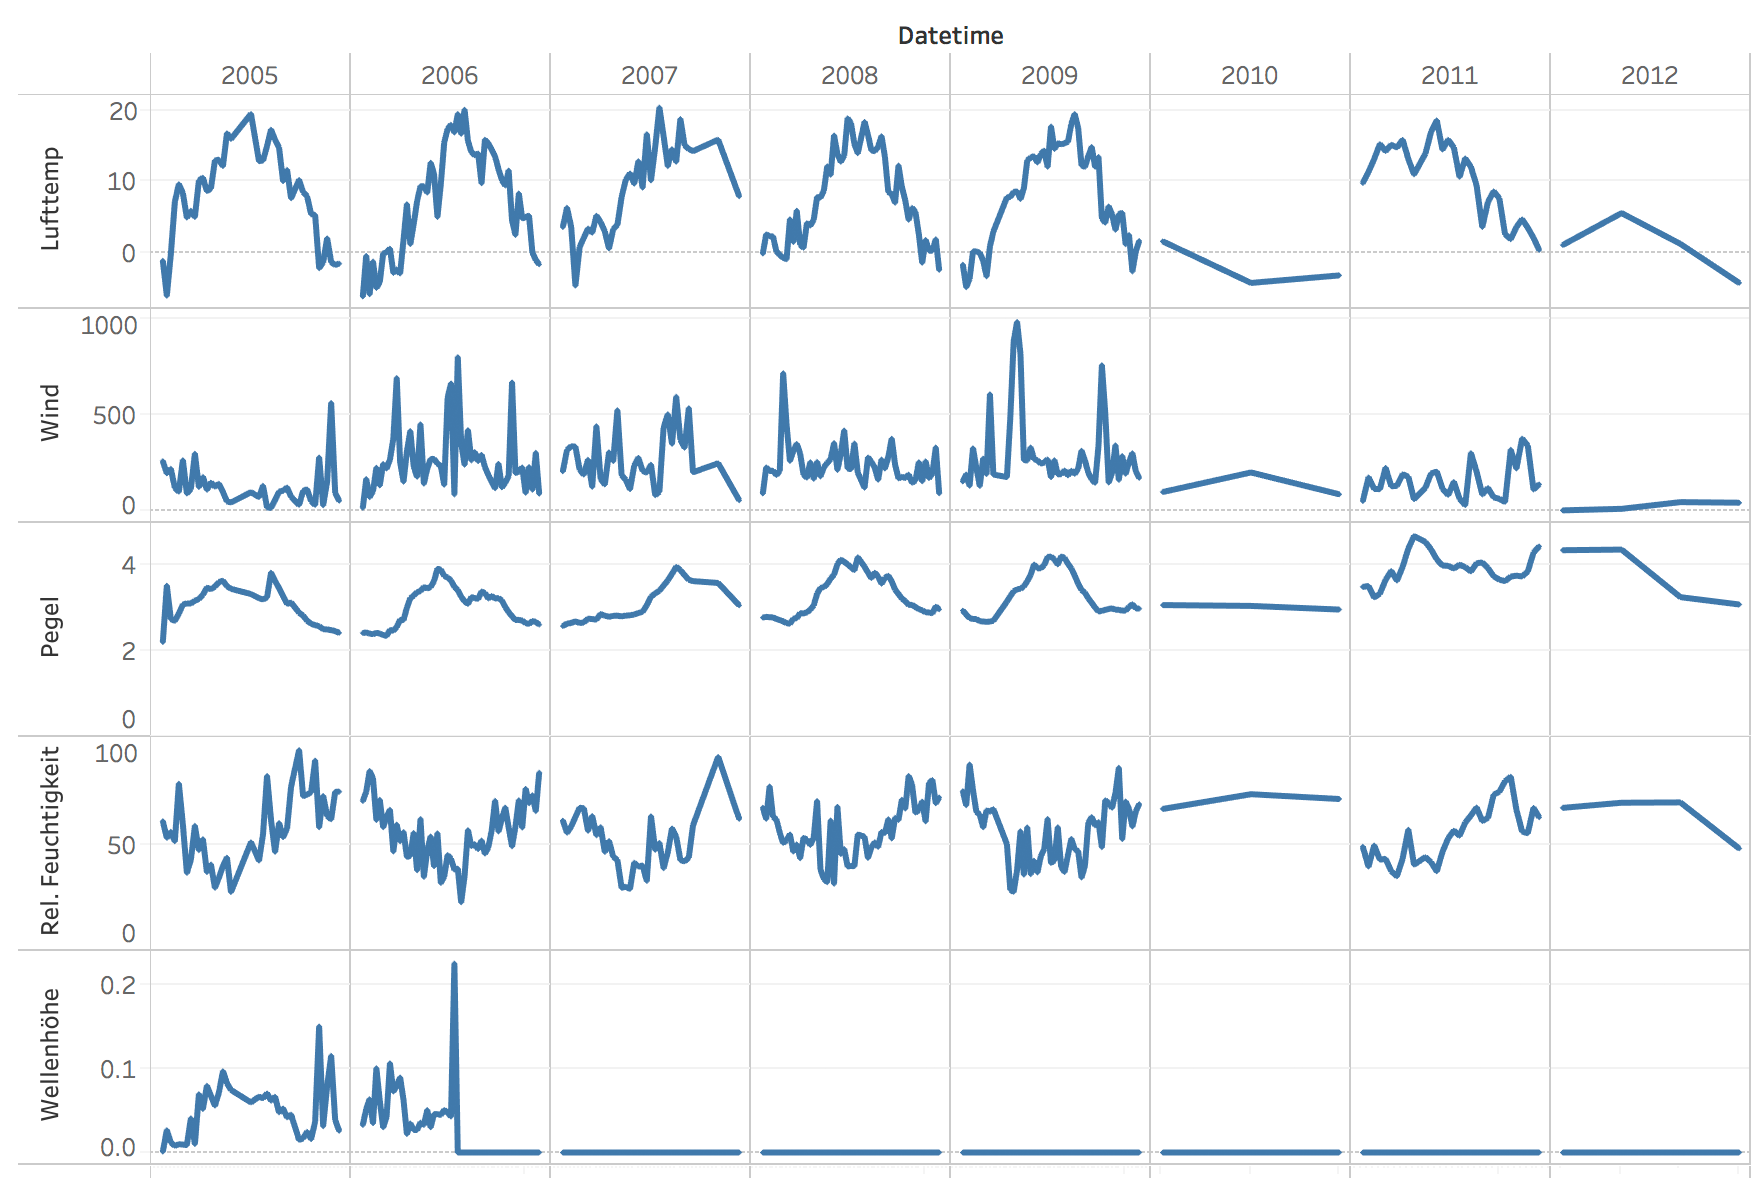
\includegraphics[width=\textwidth-2\fboxsep-2\fboxrule]{img/histAlt}}
	%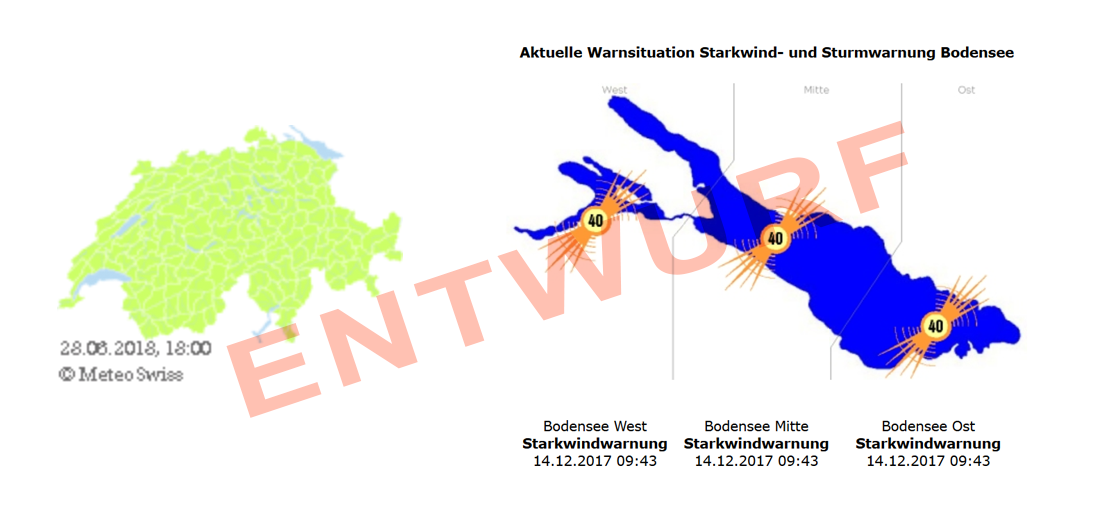
\includegraphics[width=1\linewidth]{img/sturm}
	\caption{Übersicht über die gespeicherten Daten der alten Wetterstation}
	\label{img:histAlt}
\end{figure}



\subsubsection{Pegeldaten 1953 bis 2005}
\label{subsec:pegelhistory}
Auf der Webseite wird der Pegelverlauf der letzten Jahre grafisch dargestellt. Als Grundlage diente u.a. ein Excel-File mit den Pegelständen von 1953 bis 2005. Von der alten Wetterstation liegen die Pegeldaten von 2005 bis 2009 vor und ab 2018 kommen die Messwerte der neuen Wetterstation dazu. Die Darstellung erfolgt analog Abbildung \ref{img:histPegel}. Sämtliche Datenquellen sind in einer gemeinsamen Tabelle in der Datenbank gespeichert. Die grafische Darstellung erfolgt wiederum mit Tableau, was die interaktiven Anzeige mit Filterung der Daten ermöglicht.

\begin{figure}[h!]
	\centering
  \fbox{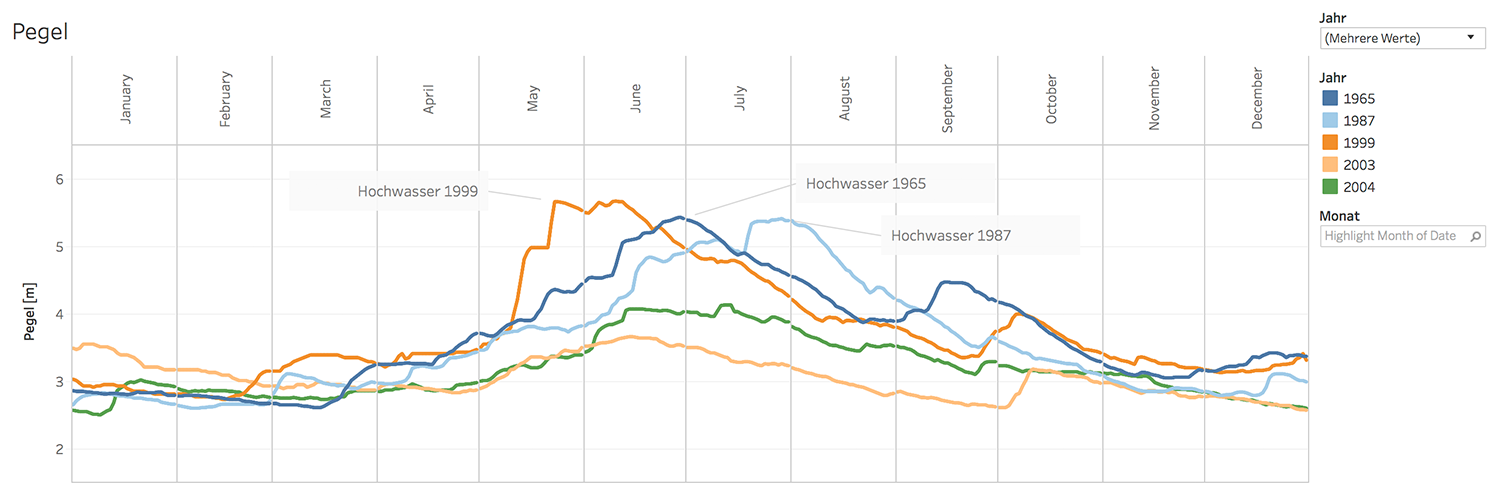
\includegraphics[width=\textwidth-2\fboxsep-2\fboxrule]{img/histPegel}}
	%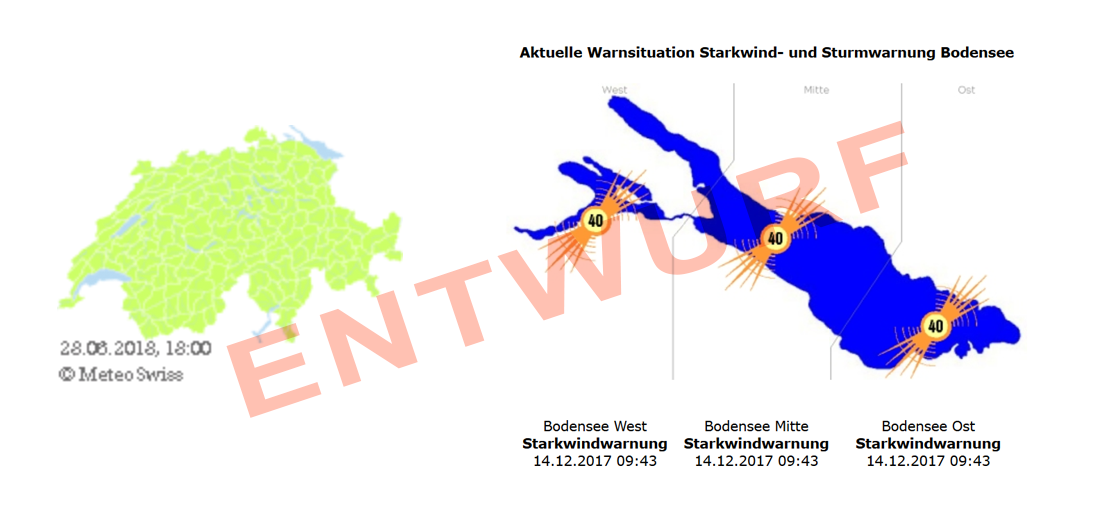
\includegraphics[width=1\linewidth]{img/sturm}
	\caption{Darstellung der historischen Pegelmesswerte}
	\label{img:histPegel}
\end{figure}



%% ############################################################################
%% Unterkapitel
%% ############################################################################
\subsection{Automatische Aktualisierung der Anzeigeelemente}
\Diskussionspunkt{Initial Values beschreiben}\newline
Die Wetterstation erzeugt jede Minute einen Datenbank-Eintrag mit den aktuellen Messwerten. Damit eine geöffnete Webseite immer auf dem aktuellen Stand ist, wird eine poll-Funktion verwendet, die selbständig alle 61 Sekunden von der API die aktuellen Werte abfragt wie in \ref{lst:poll} verkürzt dargestellt. Sobald die JSON-Daten eingetroffen sind, wird die Funktion \textit{updateData} aufgerufen, die wiederum die Anzeigeelemente und Texfelder aktualisiert. Die gesamte Aktualisierung wird asynchron mittels AJAX durchgeführt. Die Seite wird dabei nicht neu geladen, nur die Anzeigewerte. \newline

\begin{lstlisting}[label=lst:poll,caption=Automatische Aktualisierung der Werte, language=JavaScript, style=htmlcssjs]
(function poll() {
        $.get('https://api.wetter-arbon.ch/v1/')
          .done(function(response) {updateData(response);})
          .always(function() {setTimeout(poll, 61000); });
})();

function updateData(res){
        pressure_gauge.refresh(res.v1.data.pressure.value);
        $("#cwassertemp1m") = res.v1.data.watertemperature1m.value;
        ...
}
\end{lstlisting}


%% ############################################################################
%% Unterkapitel
%% ############################################################################
\subsection{Barrierefreier Zugang}
Die Wetterstation und ihre Webseite ist eine Dienstleistung der Stadt Arbon. Sie gehört der Bevölkerung und soll deshalb für möglichst alle zugänglich sein. Sowohl die \flqq Web Content Accessibility Guidelines\frqq\footnote{ \url{https://www.w3.org/TR/2008/REC-WCAG20-20081211/}} des W3C-Konsortiums, als auch die deutsche \flqq  Barrierefreie-Informationstechnik-Verordnung\frqq\footnote{ \url{https://www.gesetze-im-internet.de/bitv_2_0/BJNR184300011.html}} bieten diverse Inputs, wie die Bedienbarkeit und somit Zugänglichkeit einer Webseite verbesserte werden kann. Von einer verbesserten Zugänglichkeit profitieren nicht nur Menschen mit Einschränkungen. Es geht darum, die Webseite so zu gestalten, dass sie möglichst für alle Benutzergruppen zugänglich ist. Eine von Microsoft beauftragte Studie~\cite{ForresterResearch2004E:Abilities} der \flqq Forrester Research Inc.\frqq schätzt, dass über 60 Prozent aller Computernutzer von Barrierefreiheit profitieren können und gemäss \flqq Interface Design\frqq ~\cite{ThesmannStephan2016ID:U} wird Barrierefreiheit bald Standard sein.

\noindent
Die aktuellen Web Content Accessibility Guidelines\footnote{\url{https://www.w3.org/TR/WCAG20/}} fordern die Einhaltung von vier Designprinzipien, welche in gesamthaft zwölf Richtlinien genauer spezifiziert sind.

\begin{itemize}
\item Designprinzip 1: wahrnehmbar
\item Designprinzip 2: bedienbar
\item Designprinzip 3: verständlich
\item Designprinzip 4: robust
\end{itemize}

\noindent
Aus den Richtlinien wurden diejenigen Anforderungen ausgewählt, die auf die Webseite der Wetterstation zutreffen und die im Rahmen des CMS umsetzbar sind. Alle relevanten Anforderungen und deren Umsetzung werden im Folgenden beschrieben.

\subsubsection{Wahrnehmbarkeit}
% Richtlinie 1.1
\href{https://www.w3.org/Translations/WCAG20-de/#text-equiv}{Richtlinie 1.1} fordert, dass für alle Nicht-Text-Inhalte eine Textalternative zur Verfügung steht. Auf der Webseite mit den aktuellen Messwerten gibt es drei Typen von Nicht-Text-Inhalten: Gauges, Icons und Graphen. Bei den Gauges und Graphen werden fertige javascript-Bibliotheken verwendet. Diese stellen leider keine Möglichkeit zur Verfügung einen Alternativtext hinzuzufügen. Für die Icons, welche als \textit{img} gekennzeichnet sind, wurde das \textit{alt}-Attribut ausgefüllt, wie in Listing \ref{lst:altImg} beispielhaft dargestellt.

\begin{lstlisting}[label=lst:altImg,caption=Alternativtext für Icons, language=HTML5, style=htmlcssjs]
<img src="img/wi-humidity.svg" alt="Icon eines Barometers">
\end{lstlisting}

Wie die verwendeten javascript-Bibliotheken, bietet auch Tableau, mit welchem die interaktive Darstellung der historischen Daten erfolgt, keine Möglichkeit die Visualisierung als Text darzustellen. \newline

% Richtlinie 1.3
\noindent
\href{https://www.w3.org/Translations/WCAG20-de/#text-equiv}{Richtlinie 1.3} fordert, dass die Struktur d.h. die Zusammenhänge und die Bedeutung einer Webseite unabhängig der Formatierung erhalten bleiben. Man spricht hier auch von \textit{semantischem} Web.

Auf der Webseite wurde eine hierarchische Struktur implementiert, siehe Abbildung \ref{img:semWeb}. Die Hierarchiestufe wird einerseits erkennbar durch die Stufe der Überschriften (h1...h3) und andererseite durch die Bezeichnung der verschiedenen Inhaltsblöcke. Auf der Webseite sind zwei Hauptblöcke erkennbar, sogenannte \textit{Sektionen}. Eine Sektion beinhaltet die aktuellen Messwerte und die andere die Messdatenverläufe. Eine \href{https://www.w3.org/TR/2011/WD-html5-20110525/sections.html#the-section-element}{\textit{Sektion}} ist eine thematische Gruppierung von Elementen. Innerhalb der Sektion gibt es mehrere \href{https://www.w3.org/TR/2011/WD-html5-20110525/sections.html#the-article-element}{\textit{Artikel}}, welche einen unabhängigen Informationsblock darstellen.

\begin{figure}[h!]
	\centering
  \fbox{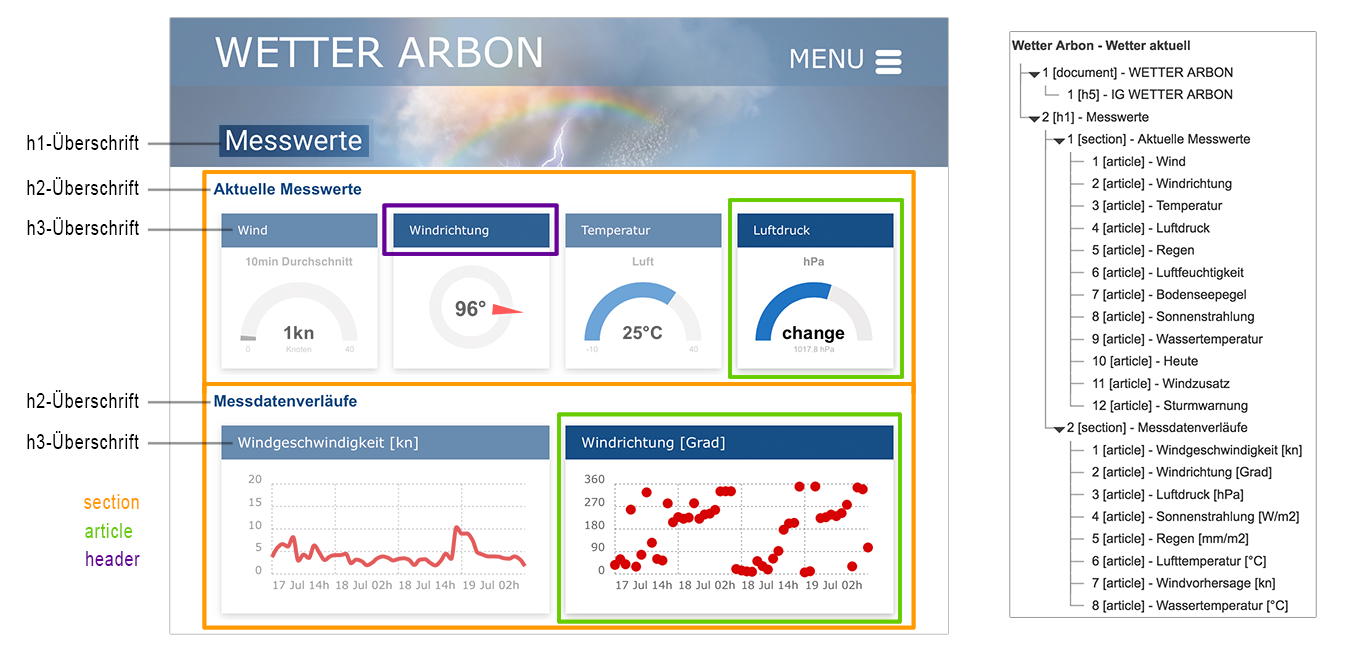
\includegraphics[width=\textwidth-2\fboxsep-2\fboxrule]{img/semWeb}}
	%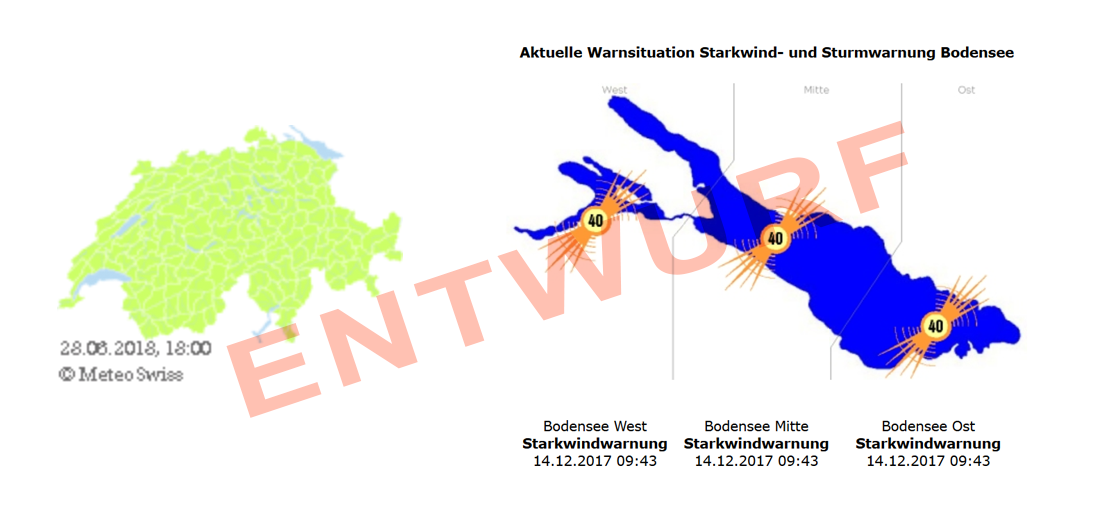
\includegraphics[width=1\linewidth]{img/sturm}
	\caption{Umsetzung der semantisches Web-Anforderung}
	\label{img:semWeb}
\end{figure}

% Richtlinie 1.4
\noindent
\href{https://www.w3.org/Translations/WCAG20-de/#visual-audio-contrast}{Richtlinie 1.4} fordert, dass die visuelle Darstellung von Text ein Kontrastverhältnis von mindestens 4,5:1 hat. Zudem muss es möglich sein die Textgrösse um bis zu 200 Prozent zu erhöhen, ohne dass dabei Inhalt oder Funktionalität verloren geht. Um diese Anforderung zu Überprüfen wurde das Firefox-Plugin \textit{tota11y}\footnote{\url{http://khan.github.io/tota11y/}} verwendet. Das Plugin ermöglicht es auf einfache Weise zu überprüfen ob die Webseite die Barrierefrei-Bediungungen erfüllt. Die Kontrastverhältnisse liegen gemäss diesem Tool zwischen 5.75 und 12.63 und sind somit in Ordnung. Da die gesamte Webseite responsive ist, stellt die Vergrösserung auf 200\% kein Problem dar.


\subsubsection{Bedienbarkeit}
\href{https://www.w3.org/Translations/WCAG20-de/#keyboard-operation}{Richtlinie 2.1} fordert, dass alle Funktionen über eine Tastaturschnittstelle bedienbar sind und das die Tastaturfokusanzeige sichtbar ist.
Da es sich bei der Webseite der Wetterstation primär um eine Anzeige handelt, ist dieses Anforderung nur für das Eingabeformular des Benachrichtiungsservice, siehe Kapitel \ref{notifications}, relevant. Dieses ist problemlos mittels Tastatur bedienbar. \newline

\noindent
\href{https://www.w3.org/Translations/WCAG20-de/#navigation-mechanisms}{Richtlinie 2.4} fordert, dass Webseiten einen zweckbeschreibenden Titel aufweisen und dass Zwischentitel den Inhalt und Zweck des entsprechenden Blocks beschreiben. Wie in Abbildung \ref{img:semWeb} wurde besitzt die Webseite sowhol einen Seitentitel, als auch Zwischentitel.


\subsubsection{Verständlichkeit}
\href{https://www.w3.org/Translations/WCAG20-de/#minimize-error}{Richtlinie 3.3} fordert, dass Eingabefehler automatisch erkannt und dem Benutzer angezeigt werden. Zudem sind Korrekturvorschläge anzuzeigen. Diese Anforderung betrifft insbesondere das Formular des Benachrichtigungsservices, welcher in Kapitel \ref{notifications} beschrieben wird. Diese Anforderung wird erfüllt, wie in Abbildung \ref{img:notificationFE} rechts, dargestellt.


\subsubsection{Robustheit}
\href{https://www.w3.org/Translations/WCAG20-de/#ensure-compat}{Richtlinie 4.1} fordert, dass Inhalten, die mit Hilfe von Markup-Sprachen implementiert wurden,  vollständige Start- und End-Tags haben. Es sind keine doppelten Attribute vorhanden und alle IDs sind eindeutig. Diese Anforderung wurde ebenfalls vollständig umgesetzt. Beispielhaft ist dies in Listing \ref{lst:gaugeHTML} ersichtlich.

\section{Datenbank / back end / cronjobs}
In diesem Kapitel wird aufgezeigt welche Änderungen an der Datenbank vorgenommen werden und wo diese überall zum Einsatz kommen. Zudem wird aufgezeigt, wie diese zusätzlichen Anwendungen entwickelt wurden. Vor der Umstrukturierung der Datenbank waren die Tabellen unübersichtlich aufgebaut. Nach der Umstrukturierung soll die Datenbank primär für folgende Aufgaben ausgelegt sein:
\begin{itemize*}
\item API
\item Dreitage Rückschau der verschiedenen Sensoren
\item Historische Daten
\end{itemize*}

Die Aufgabe der Datenbank ist es, den Umgang mit den Daten einfacher zu gestalten. Sei es in Bezug auf die Aufbereitung der historischen Daten oder für den Aufbau der API, welche einfach erweiterbar sein soll.



%% ############################################################################
%% Unterkapitel
%% ############################################################################
\subsection{Datenerfassung}
% Ueberischt über alle Kanäle -> was wird wie erfasst

\begin{figure}[htbp!]
  \fbox{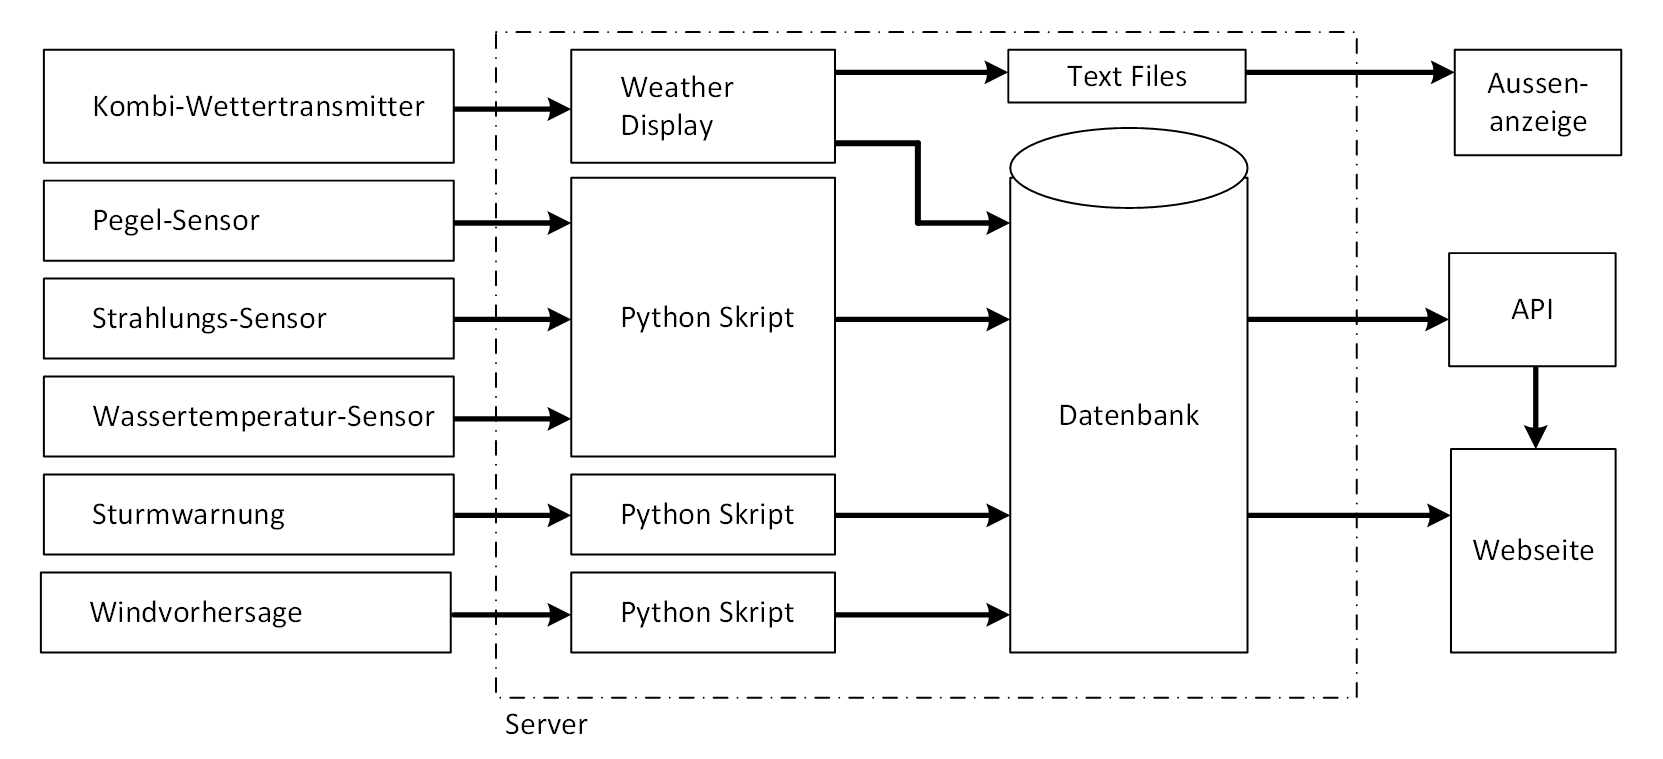
\includegraphics[width=\textwidth-2\fboxsep-2\fboxrule]{img/datenerfassung}}
	\centering
	\caption{Datenerfassung}
	\label{img:datenerfassung}
\end{figure}




\subsubsection{Erfassung der Daten des Wetter-Transmitters}
Die Daten des Wetter-Transmitters werden weiterhin von WeatherDisplay über eine virtuelle serielle Schnittstelle abgerufen sowie aufbereitet. Damit die Daten im Minutentakt in der Datenbank gespeichert werden. Für die Umgestaltung der Datenbank wurde auch die Konfiguration im WeatherDisplay angepasst. \Diskussionspunkt{Bild Weatherdisplay Konfiguration} In der Konfiguration können die Datenpunkte welche eingetragen werden sollen selektiert werden. \Diskussionspunkt{Weitere Konfigmöglichkeiten aufzeigen}

Kann ein Datenbankeintrag nicht erstellt werden, weil es zu wenig Einträge hat oder aus anderen Gründen wird dies, wie später im Kapitel Funktionsüberwachung mit Mail-Service \ref{kap:Funktionsüberwachung}, beschrieben im Cronjob abgefangen.

\subsubsection{Einlesen von Pegel- und Strahlungsmesswerten}
Wassertemperatur, Strahlungssensor und Pegelsenoren sind alle an einem Web-IO angeschlossen, welche die analogen Werte per Web-Schnittstelle zur Verfügung stellt. Die Abfrage erfolgt einmal pro Minute durch ein Python-Skript, wie in Listing \ref{lst:webIo} dargestellt. Der URL-Request wird mittels cURL ausgeführt. Die Abfrage ist für alle genannten Sensoren die gleiche, nur die URL unterscheidet sich je nach Sensor. Die Abfragen sind nach dem try... catch - Prinzip aufgebaut, sodass das Skript weiterläuft auch wenn vom Web-IO keine Antwort eintrifft.

\begin{lstlisting}[label=lst:webIo,caption=Python-Script zur Web-Abfrage des Pegel-Messwerts, language=python, style=py]
try:
    buffer = StringIO()
    c = pycurl.Curl()
    c.setopt(c.URL, 'http://webcam.wetter-arbon.ch:50506/single1')
    c.setopt(c.WRITEDATA, buffer)
    c.perform()
    c.close()
    requestMeasurement = buffer.getvalue()
\end{lstlisting}


\subsubsection{Abgreifen der Sturmwarndaten} % screen scrapping
Die Sturmwarndaten werden periodisch mittels Python-Skript ausgelesen. Als Web-Scrapper kommt die Python-Bibliothek \href{https://www.crummy.com/software/BeautifulSoup/}{\emph{BeautifulSoup}} zum Einsatz. Das Auslesen von Webseiten wird auch \emph{web scraping} genannt. Die Idee dahinter ist, die gewünschte Information auf Grund ihrer Element-Bezeichnung (\texttt{<td>}), ihres Attributs (\texttt{class="titelfett"}) oder Hierarchistufe (\texttt{tr:nth-of-type(4)}) eindeutig zu identifizieren. Um diese eindeutige Identifikation herauszufinden wurde das Google Chrome-Plugin \href{https://selectorgadget.com/}{\emph{SelectorGadget }} verwendet. Listing \ref{lst:kttgCrawler} zeigt die gesamte Abfrage. Darin ist das Problem dieser Methode gut erkennbar. Ändert die URL oder die Bezeichung bzw. Struktur der Seite, liefert das Skript nicht mehr die gewünschten Daten. Da das Web-Scrapping jedoch die einzige kostenlose Möglichkeit darstellt um die Daten zu erhalten, muss dieses Risiko akezptiert werden.


\begin{lstlisting}[label=lst:kttgCrawler,caption=Web-Scrapper für die Sturmwarndaten, language=python, style=py]
page = requests.get('http://www.kttg.ch/kapo/htm/stwarn.shtml')
soup = BeautifulSoup(page.text, 'html.parser')

# Einschaltzeit auslesen
soup.select('table tr:nth-of-type(4) td'):

# Status auslesen
soup.select('.titelfett strong'):
\end{lstlisting}


\subsubsection{Windvorhersagedaten}
Die Abfrage der Datenban stellt sich als recht kompliziert heraus. Sodass entschieden wurde eine VIEW einzusetzten. Diese wird dynamisch bei Aufrufen erzeugt und enthält die gewünschten Daten. Der SQL-Befehl für die Erzeugung der VIEW ist vereinfacht in Listing \ref{lst:viewForecast} aufgeführt. Primär gibt es zwei Bediungungen. Erstens sollen nur die Dreitageverhersagewerte verwendet werden und zweitens sollen die Vorhersagewerte verwendet werden, die am nächsten bei der aktuellen Zeit liegen. Da das Vorhersageintervall 3 Stunden beträgt ist die Verhersage maximal 1.5 Stunden verschoben.

%View erstellen
\begin{lstlisting}[label=lst:viewForecast,caption=Erzeugung der VIEW für den Forecast-Vergleich, language=SQL, style=htmlcssjs]
SELECT *
FROM 'tblcompwindfinder'
WHERE
(datetime + interval 3 day) <= now() #heute vor drei Tagen
AND
abs(timediff(datetime,now())) <= 13000) #innerhalb +/- 1.5h
ORDER BY datetime DESC
LIMIT 3
\end{lstlisting}


%% ############################################################################
%% Unterkapitel
%% ############################################################################
\subsection{Datenspeicherung}
Für die Datenspeicherung stellt Hostpoint, der Webhosting-Provider der Wetterstation, seinen Kunden eine MariaDB Version 10.1 mit dem Administrationstool phpMyAdmin zur Verfügung. MariaDB ist eine relationales Open-Source-Datenbankverwaltungssystem und basiert auf MySQL.

Die Datenbank wurde komplett neu aufgebaut. Im Folgenden werde die einzelnen Tabellen und deren Struktur erklärt.

%Für die Umstrukturierung wurde von der Methodik aus dem Artikel Grundlagen und Entwurf \cite{Datenbanken:GrundlagenUndEntwurf:VeikkoKrypczyk} gebrauch gemacht.
%Wie in Introduction to relational Databases \cite{IntroductionToRelationalDatabases:MariaDB} beschrieben wird,

\subsubsection{Aufbau und Inhalt der Datenbank}
Die Datenbank besteht aus mehreren Tabellen mit unterschiedlichem Inhalt. Die Auflistung sämtlicher Tabellen mit einer Beschreibung des Inhalts befindet sich in Tabelle\,\ref{table:dbtabellen}. Die obersten vier Tabellen werden zur Speicherung der Messwerte/Zusatzinformationen verwendet. Anschliessend kommen die drei Tabellen für die historischen Daten und zum Schluss zwei Tabelle, die für den Benachrichtungsservice und die Webcam benötigt werden.
%\Diskussionspunkt{Warum wurde keine zweite DB für Benachrichtigungsservice und Webcam erstellt? Zweite DB mit igwetter_Services?}

% Datenbank-Tabellen
\begin{table}[htbp!]
  \setlength\extrarowheight{3pt} % for a more "open" look
  \begin{tabularx}{\textwidth}{|>{\RaggedRight\hspace{0pt}}p{4.5cm}|X|}

  \hline
  %\textbf{Tabelle}
  & \bfseries Beschreibung \\

  \hline
  \textbf{tblwettertransmitter}
  & Messwerte des Wettertransmitters \\

  \hline
  \textbf{tblextsensors}
  & Messwerte der Sensoren (Bsp. Pegel) \\

  \hline
  \textbf{tblmisc}
  & Daten von Dritten (Bsp. Sturmwarnung) \\

  \hline
  \textbf{tblcompwindfinder}
  & Windvorhersagewerte von Windfinder \\

  \hline
  \hline
  \textbf{tbldatemaster}
  & Daten vom 1.1.2015 bis 31.12.2035 im Minutenabstand \\

  \hline
  \textbf{tblhistorical}
  & Messwerte zusammengefasst auf 1 Eintrag/h \\

  \hline
  \textbf{tblwaterlevelhistorical}
  & Pegelwerte von 1953 bis heute 1 Eintrag/d\\

  \hline
  \hline
  \textbf{tblnotifications}
  & Abos des Benachrichtigungsservices \\

  \hline
  \hline
  \textbf{tblqueue}
  & Warteschlange der Webcam \\

  \hline
  \end{tabularx}
  \caption{Datenbanktabellen und deren Inhalt}
  \label{table:dbtabellen} % label muss NACH caption stehen!!!!
\end{table}

\noindent
Die Tabellen haben untereinander keine Verknüpfung (Relation), sondern sind alle eigenständig. Das einzige, was sie verbindet ist der Zeitstempel des Messzeitpunkts. Es wird deshalb auf die Erstellung eines ER-Modells, wie in Datenbanken Grundlagen und Design \cite{FrankGeisler2011mitpu} beschrieben, verzichtet. In Abbildung\,\ref{img:tabellenstruktur} ist beispielhaft die Struktur der Tabelle \emph{tblextsensors} aufgeführt. Als Primärschlüssel wird jeweils der Zeitstempel des Messzeitpunkts verwendet. Da der Primärschlüssel ein UNIQUE-Wert ist, wird verhindert, dass es zwei Einträge mit dem selben Zeitstempel gibt. Das komplette relationale Datenmodell mit allen Entitäten und deren Attributen befindet sich in Anhang\,\ref{anhang:relationalesDatenbankmodell}.

\begin{figure}[htbp!]
  \fbox{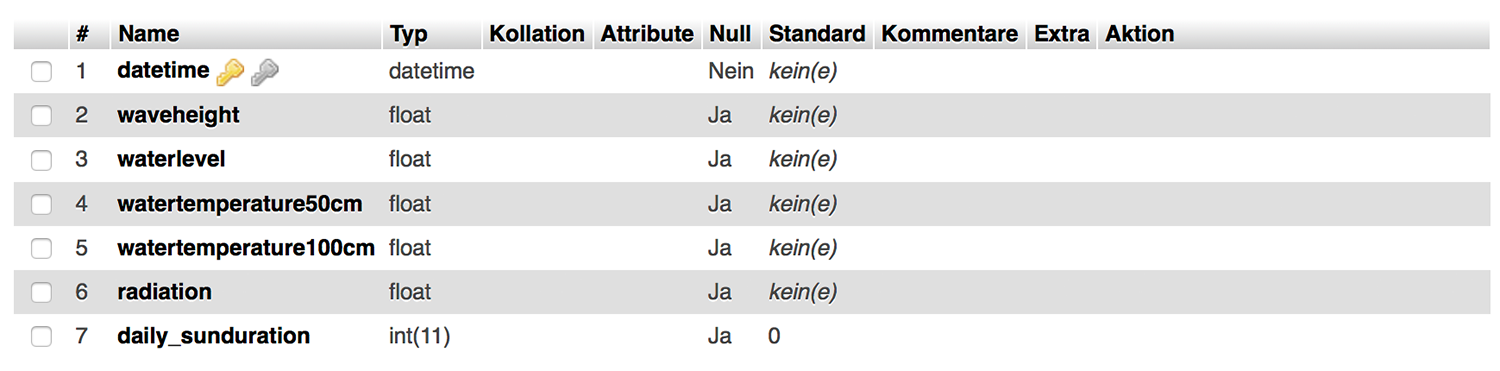
\includegraphics[width=\textwidth-2\fboxsep-2\fboxrule]{img/tabellenstruktur}}
	\centering
	\caption{Struktur der Tabelle \emph{tblextsensors}}
	\label{img:tabellenstruktur}
\end{figure}

%Die Normalisierung ist, wie in Datenbanken Grundlagen und Design \cite{FrankGeisler2011mitpu}, ein Prozess mit deren Hilfe die Datenbankstruktur optimiert wird und hilft dabei Datenredundanzen zu vermeiden. Da bei der Datenbank nur das Datum redundant ist, ist eine Normalisierung nicht notwendig.
%Das relationale Datenmodell unterscheidet sich in der Struktur nicht bedeutend vom ER-Modell. Der Unterschied  ist, dass die Primärschlüssel und die Datentypen festgelegt werden. Die sogenannten Schlüssel sind im relationalen Datenmodell auch ein wichtiges Merkmal. Bei zukünftigen Datenbankeinträgen sind entscheidend die Schlüssel, so kann verhindert werden, dass für einen gewissen Zeitpunkt nochmals Datensätze geschrieben werden.
%Die drei konzipierten Tabellen konnten wie gewünscht umgesetzt werden. Der Code für die Umsetzung der Tabellen, kann aus dem Anhang \ref{anhang:Datenbankcode} entnommen werden.\\


\subsubsection{Aggregation der historischen Daten}
Bei der Wetterstation fallen pro Minute rund 40 Datenpunkte an, die gespeichert werden. Pro Jahr sind dies über 21 Millionen Datenpunkte. Damit die Anzeige der historischen Messwerte nicht so viele Daten laden muss, werden die Messdaten periodisch zusammengefasst.
\newline

% Tabelle mit Minutenwerten
% Tabelle mit Tageswerten
% Wie funktioniert das Zusammenfassen der Daten -> SQL-Befehle

% \paragraph{Konzept}
\noindent
Die minütlich gespeicherten Messdaten werden einmal pro Stunde zusammengefasst und in die Tabelle mit den historischen Werten \emph{tblhistorical} geschrieben. Für die Aggregation wird die Median-Funktion verwendet um den Einfluss von Messfehlern zu reduzieren. Einmal pro Tag werden zudam die Pegeldaten des gesamten Tags gemittelt und in die Tabelle \emph{tblwaterlevelhistorical} geschrieben, wie in Abbildung\,\ref{img:historical} dargestellt.

\begin{figure}[htbp!]
  \fbox{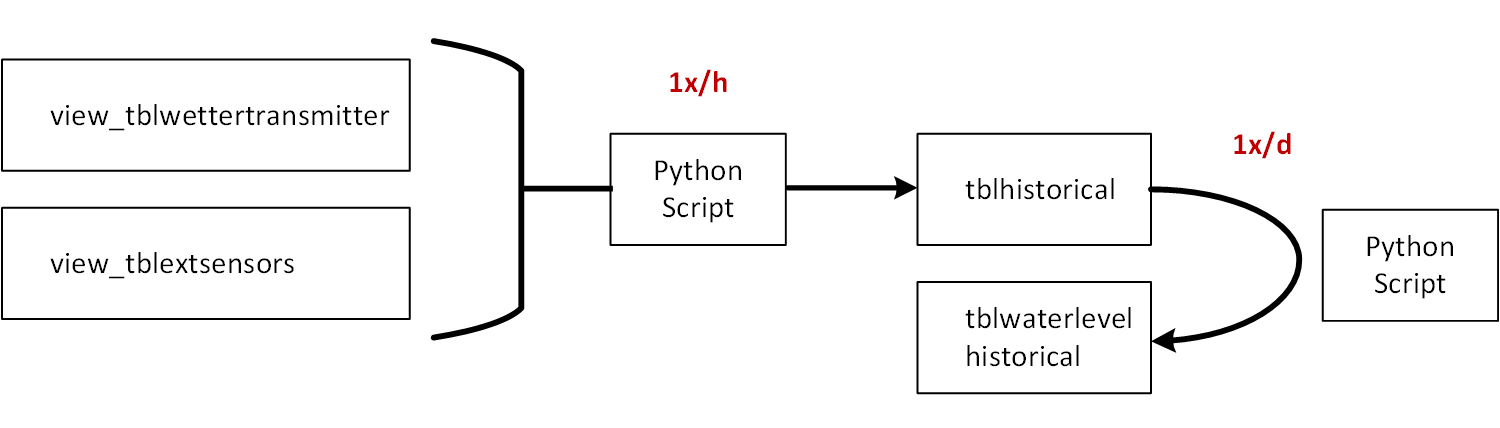
\includegraphics[width=\textwidth-2\fboxsep-2\fboxrule]{img/historical}}
	\centering
	\caption{Konezpt der Datenaggregation}
	\label{img:historical}
\end{figure}


% \paragraph{LEFT JOIN}
Das Script, welches die minütlichen Daten zu Stundendaten aggregiert greift nicht direkt auf die Messwerttabellen zu, sondern auf sogenannte VIEWs. Eine VIEW ist eine virtuelle Tabelle. Sie enthält keine Daten, sondern verweist auf die zugrundeliegenden Basistabellen. VIEWs ermöglichen es komplexere Abfragen zu vereinfachen und mehrere Tabellen über JOIN-Verknüpfungen zu einer einzigen Tabelle zusammenzufassen.

\begin{figure}[htbp!]
  \fbox{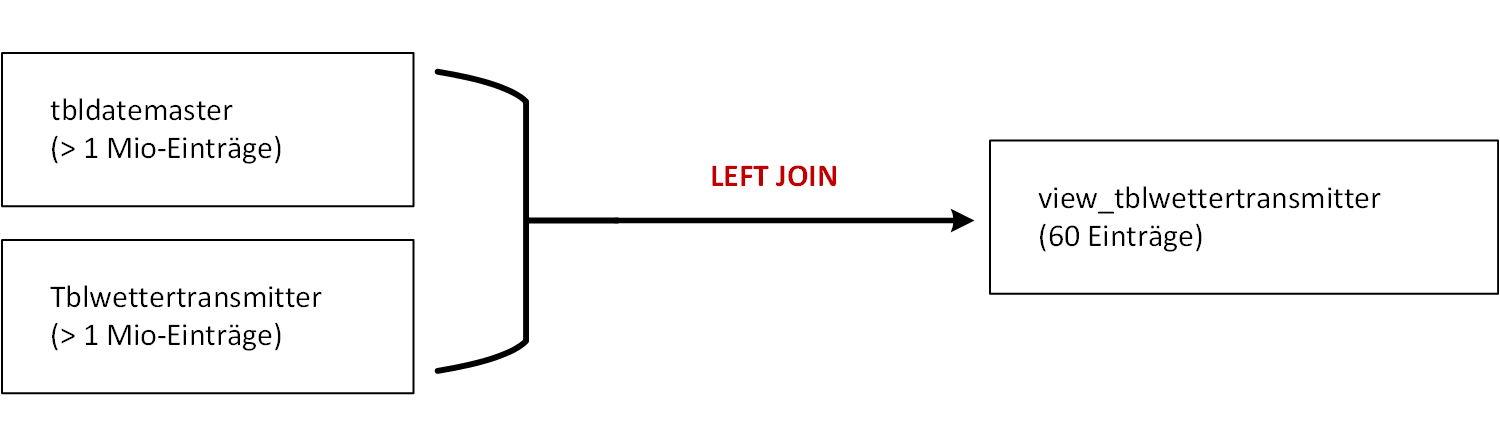
\includegraphics[width=\textwidth-2\fboxsep-2\fboxrule]{img/leftjoin}}
	\centering
	\caption{Konezpt der Datenaggregation}
	\label{img:leftjoin}
\end{figure}


Die beiden VIEWs, die für die Aggregation benötigt werden beinhalten jeweils genau 60 Einträge. Einen für jede Minute der vergangenen Stunde. Damit immer für jede Minute ein Eintrag vorhanden ist, auch wenn zum Beispiel der Sensor aus irgendeinem Grund keine Messwert geliefert hat, wurde ein LEFT JOIN mit der Datemaster-Tabelle erstellt. Diese Tabelle enthält sämtliche Datum/Zeit Einträge von 2015 bis 2035 im Minutenabstand.



%Bevor sich Gedanken um die Datensicherheit gemacht werden, sollten die Bedingungen an den Speicherplatz klar sein. Während der Laufzeit werden grosse Mengen an Daten in die Datenbank geschrieben. Vor der Neukonzipierung werden täglich 1440 Datensätze gespeichert. Das bedeutet jede Minute einen Datensatz. Ein Datensatz beinhaltet 65 Einträge, die gesamte relevante Datenbank igwetter wettertest benötigt (Stand 2018-04-24) 323.2  Mb. Die Tabelle wx data, beinhaltet die Minutenwerte des Wettertransmitters, benötigt davon (Stand 2018-04-24) 311.9 Mb, daraus erfolgt das ein Datensatz ca 0.025 Mb benötigt. Für den Speicherplatz, welcher 50 Gb bietet, stellt dies kein Problem dar. Hochrechnet reicht der Platz für die kommenden 45 Jahren.


% Die Herausforderung bei der Umsetzung war es, dass die historische Tabelle, welche aus den beiden Tabellen tblwettertransmitter und tblextsensors bestehen, mittels einer Query zusammenzubringen.

% Das Problem war die Zeit. Die Daten des Wettertransmitters werden Konfigurationsbedingt, nicht auf die Minute genau, sondern 31 Sekunden später geschrieben. Bei einem LEFT JOIN, welches über die Zeit geht, werden auch die Sekunden angeschaut. Nach mehreren gescheiterten Versuchen, ist es anschliessend gelungen, eine passende Query wie in \ref{lst:LeftJoinQuery} zu entwickeln.

% Zudem wird eine historische Tabelle erstellt, diese soll, die zu stündlich aufbereiteten Daten aus den beiden Tabellen enthalten.
% Um die historische Tabelle ohne Ausfälle zu füllen wird eine Tabelle entstehen, welche alle Zeitstempel von 2015 bis 2030 beinhaltet. Welche Datenpunkte übernommen werden, kann aus dem Anhang \ref{anhang:Datenbankschema} entnommen werden.\\

% Beim Modell der historischen Daten sieht das ganze anders aus (siehe Abb. \ref{img:ER_Modell historische Daten}). Hier beinhaltet jeder Zeitstempel, den Median, sowie die Extremwerte der Daten vom Wettertransmitter und die der externen Sensoren.

% Zusätzlich sollen die Daten, welche weiterhin im Minutentakt geschrieben werden, so aufbereitet werden, dass Benutzer auf der neu erstellen historischen Webpage die Wetterdaten der vergangenen Jahre einsehen können.


% \begin{lstlisting}[label=lst:LeftJoinQuery,caption=Json Struktur, language=JavaScript, style=htmlcssjs, mathescape]
% SELECT * FROM `DateMaster`
% LEFT JOIN `tblwettertransmitter`
% ON MINUTE(dt) = MINUTE(datetime)
% WHERE ((`DateMaster`.`dt` > (now() - interval 2 hour))
% AND((`tblwettertransmitter`.`datetime` > (now() - interval 2 hour))
% AND (hour((now() - interval 1 hour)) = hour(`tblwettertransmitter`.`datetime`)))
% AND (hour((now() - interval 1 hour)) = hour(`DateMaster`.`dt`))
% AND (`DateMaster`.`dt` < now()))
% order by `DateMaster`.`dt` desc
% \end{lstlisting} */


%% ############################################################################
%% Unterkapitel
%% ############################################################################
\subsection{Automatisierung der repetitiven Aufgaben (Cronjobs)}

%wiederkehrende Aufgaben – sogenannte Cronjobs – zu automatisieren.
% Der Cron-Daemon dient der zeitbasierten Ausführung von Prozessen in Unix und unixartigen Betriebssystemen wie Linux

Die Wetterstation basiert auf vielen repetitiven Aufgaben wie zum Beispiel das minütliche Einlesen der Messdaten. Linux, welches auf dem Hostpoint-Server verwendet wird, bietet mit dem Cron-Daemon ein Werkzeug um zeitbasiert Befehle beziehungsweise Skripte (Cronjobs) auszuführen. Eine Liste sämtlicher Cronjobs, die die Wetterstation verwendet ist in Tabelle \ref{table:cronjobs} dargestellt. Um einen Cronjob zu definieren muss einerseits das auszuführende Skript angegeben werden und der Zeitpunkt, zu dem es ausgeführt werden soll. Es kann zwischen Minute, Stunde und Tag gewählt werden. Ein Stern (*) bedeutet zu jeder Minute/Stunde/Tag. Die historischen Daten (\emph{historical.py}) werden beispielsweise zu jeder Stunde jeweils um 5 Minuten nach zusammengefasst. Die Windvorhersage von Windfinder (\emph{forecastWindfinder.py}) werden alle drei Stunden abgefragt (02:37, 05:37 usw.).


%Viele Funktionen werden mit Cronjobs ausgeführt. Wie von Hostpoint \cite{Hostpoint:CronjobsEinrichten} dargestellt, werden Cronjob für wiederkehrende Abläufe verwendet. Anders formuliert, kann ein Script zu einem bestimmten Zeitpunkt automatisiert ausgeführt werden. Es wird angegeben zu welchem Zeitpunkt oder in welchem Intervall das Programm ausgeführt werden soll. Der Rest übernimmt dann anschliessend der Cronjob. In diesem Fall, das Auslesen der externen Sensordaten, das erstellen der historischen Daten und das auslesen der Sturmwarnung. Auf Hostpoint kann mittels Knopfdruck ein Cronjob erstellt werden. Dabei kann auch gleich konfiguriert werden, zu welcher Zeit ein Cronjob ausgeführt werden soll (Tabelle \ref{table:cronjobs}).


% Tabelle Cronjobs
\begin{table}[htbp!]
  \setlength\extrarowheight{3pt} % for a more "open" look
  \begin{tabularx}{\textwidth}{|X|>{\RaggedRight\hspace{0pt}}p{3.5cm}|X|>{\RaggedRight\hspace{0pt}}p{5.5cm}|}

  \hline
  %\textbf{Tabelle}
  \bfseries Minute
  & \bfseries Stunde
  & \bfseries Tag
  & \bfseries Befehl/Skript \\

  %\hline
  \hline
  37
  & 2,5,8,11,14,17,20,23
  & *
  &  forecastWindfinder.py \\


  \hline
  *
  & *
  & *
  & sturmwarnung.py \\

  \hline
  *
  & *
  & *
  & externSensors.py \\

  \hline
  *
  & *
  & *
  & notifications.py \\

  \hline
  5
  & *
  & *
  & historical.py \\

  \hline
  7
  & 0
  & *
  & historicalWaterlevel.py \\


  \hline
  \end{tabularx}
  \caption{Konfiguration der Cronjobs}
  \label{table:cronjobs} % label muss NACH caption stehen!!!!
\end{table}


Die erwähnten Cronjob sind die wichtigsten, werden diese nicht durchgeführt, werden auch keinen Daten ausgelesen bzw. erstellt. Neben diesen drei Cronjobs bestehen noch zwei weitere. Diese lesen die Wettervorhersage für den Vergleich aus und schreiben die Daten in die Datenbank.

%Rechnern welche nicht durch einen Dauerbetrieb gekennzeichnet sind, kommen meist andere Varianten wie anacron zum Einsatz.



% ############################################################################
%% Unterkapitel
%% ############################################################################
\subsection{Zeit}
\subsubsection{Zeitsynchronisation}
% welche Daten erhalten von wo einen Zeitstempel?
% woher erhalten diese Geräte die Zeit? Zeitserver?


\subsubsection{Formatierung von Datum/Zeit}

\subsubsection{Zeitumstellung}
Da in der Schweiz Sommer- und Winterzeit herrscht, besteht auch die Problematik der Zeitumstellung. Für die Datenbank besteht das Problem, dass die Tabellen nur einen Datumzeit enthalten dürfen. So entsteht die Problematik im Winter, da wenn die zurück gestellt wird doppelte Einträge entstehen. Wird in die historische Daten geschaut, fällt auf das diese Zeitumstellung nie berücksichtigt wurde. Zudem ist die Zeitumstellung in der Nacht, also für viele Benutzer eher uninteressant. Somit spielt es keine Rolle, dass die Daten bei der Zeitumstellung verloren gehen.




%% ############################################################################
%% Unterkapitel
%% ############################################################################
\subsection{Datenbanksicherheit (Datenmanipulation und -verlust)}


\subsubsection{Angriffssicherheit}
Bei der Recherche nach Datenbanksicherheit taucht immer wieder das Wort Injection auf. Laut den OWASP\footnote{OWASP: Open Web Application Security Project} Top 10, einer Liste\footnote{ \url{https://www.owasp.org/index.php/Category:OWASP_Top_Ten_Project}}, welche die wichtigsten Sicherheitsrisiken von Web-Applikationen aufzeigt, ist SQL-injection seit Jahren auf Platz 1. SQL-Injection ist eine Methode eine Datenbankabfrage so zu manipulieren, dass der Angreifer Daten ausspähen oder verändern kann.

Bei der Wetterstation Arbon, sind keine persönlichen oder sicherheitsrelevanten Daten in der Datenbank gespeichert. Somit ist diese aus Sicht eines potentiellen Angriffes eher uninteressant. Dennoch sollten die Daten hinreichend geschützt sein, um einen Datenverlust beziehungsweise eine Datenmanipulation zu verhindern.

Die Zugriffe auf die Datenbank sind so gestaltet, dass nur serverseitig darauf zugegriffen wird. Die Darstellung der Anzeigen auf der Webseiten werden über die API erstellt. Die API wiederum ist so aufgebaut, dass ein PHP-Skript auf dem Server die Daten aus der Datenbank abgreift und sie richtig formatiert. Somit kann sichergegangen werden, dass keine SQL-Injection möglich ist. Wie im Kapitel Daten der neuen Wetterstation mit Tableau \ref{kap:Tableau} erwähnt, müssen die Daten für das Tableau manuell übertragen werden. Dies bedeutet, dass für die historische Seite kein Datenbankzugriff notwendig ist. Lediglich bei der Warteschlang der Webcam und beim Benachrichtigungsservice werden Daten direkt in die Datenbank geschrieben beziehungsweise daraus gelesen. In diesem Fall werden die Eingaben maskiert wie in Listing\,\ref{lst:maskierung} dargestellt.

\begin{lstlisting}[label=lst:maskierung,caption=Maskierung von Datenbank-Eingaben, language=PHP, style=PHP]
$threshold = mysql_escape_string($_POST['threshold']);
\end{lstlisting}


\subsubsection{DB-Nutzer Konzept}
welche Nutzer gibt es und welche Rechte haben sie -> theoretisch erklären

\subsubsection{Backup}
Um die Datenbank gegen einen allfälligen Datenverlust zu sichern, ist ein Backup von wichtiger Bedeutung. Deswegen ist das Backup ein weiterer Aspekt gegen den Verlust von Daten. Hierbei sind folgende Fragen relevant:
\begin{itemize}
\item Welche Daten sollen gesichert werden?
\item Wie oft sollten die Daten gesichert werden?
\item Wie bzw. wo sollte das Backup gelagert werden?
\end{itemize}

Da alle Daten in der DB gleich relevant sind, sollten auch alle so behandelt werden und im Backup vorhanden sein. Dabei muss aber entschieden werden, ob ein tägliches Backup Sinn machen würde. Da die Wetterstation von einem Verein betrieben wird, ist es wichtig den Aufwand mit dem Ertrag zu vergleichen. Zusätzlich sollte das Backup nicht auf dem Server des Providers gespeichert werden, sollte etwas mit dem Server nicht in Ordnung sein, sind diese Daten auch weg. Deswegen ist es wichtig auch ein 'externes' Backup zu erstellen. Hostpoint bietet für das Backup verschiedene Varianten:
\begin{itemize}
\item Cronjob
\item Backup auf Knopfdruck
\item Kostenpflichtige Wiederherstellung aller Daten
\end{itemize}


Um den Aufwand klein zu halten, wird empfohlen ein monatliches Backup mit der Backup Funktion auf Knopfdruck zu erstellen und dieses auf einer Festplatte zu speichern (Abb. \ref{img:backup}).

\begin{figure}[htbp!]
  \fbox{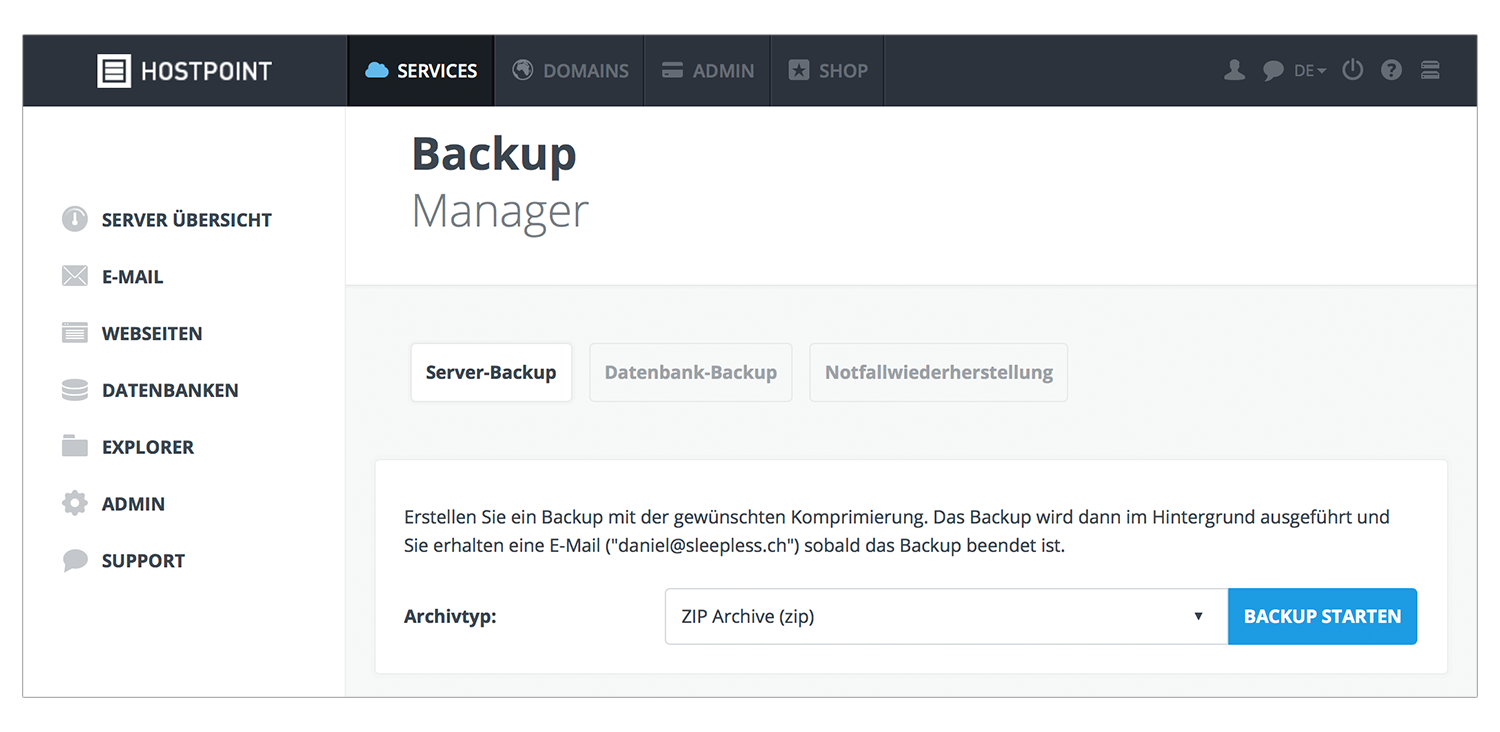
\includegraphics[width=\textwidth-2\fboxsep-2\fboxrule]{img/backup}}
	\centering
	\caption{Backup auf Knopfdruck von Hostpoint}
	\label{img:backup}
\end{figure}

Sollte trotzdem mal das Backup nicht funktionierten oder vergessen gegangen sein, kann auf den Hostpoint-Service ( Abb.\ref{img:Notfallwiederherstellung}) züruck gegriffen werden. Diese erstellen selber ein tägliches Backup, welches für 100 Franken wieder eingespielt werden kann.



Somit können sich, davon ausgehend, dass Hostpoint einen guten Job macht Kosten für bspw. ein Cloudaccount gespart werden.

%% ############################################################################
%% Unterkapitel
%% ############################################################################
\subsection{Speicherbedarf und Datenarchivierung}

In der Datenarchivierung werden die historischen Daten aufbereitet und komprimiert. Dafür ist wird von der historischen Tabelle gebrauch gemacht. Mittels einem Cronjob und dem in \ref{lst:LeftJoinQuery} codierten Left Join werden die Minuten Daten komprimiert. Anschliessend bestehen zwei Varianten:\\
\begin{itemize}
\item \textbf{Variante 1}\\
Die Daten aus den beiden Minutentabellen werden gelöscht, stehen somit nicht zu weiteren Zwecken zur Verfügung.
\item \textbf{Variante 2}\\
Die Daten aus den beiden Minutentabellen werden nicht gelöscht und können für spätere Anwendungen verwendet werden.
\end{itemize}

Da beim Server der Speicherplatz kein ausschlaggebender Punkt ist, wurde für die zweite Variante entschieden.



%% ############################################################################
%% Unterkapitel
%% ############################################################################
\subsection{Funktionsüberwachung mit Mail-Service}\label{kap:Funktionsüberwachung}
Um die Funktion der Software zu gewährleisten, sollte bei einem Absturz der Verantwortliche für die IG bei der IG benachrichtigt werden. Folgende Funktionen müssen bei einem Absturz eine Meldung geben.
\begin{itemize}
\item Einlesen Sensordaten extern
\item Einlesen Wettertransmitter Daten
\item Erstellung der stündlichen historischen Daten
\end{itemize}
Die Aufgezählten Funktionen werden alle bis auf das Einlesen der Wettertransmitter Daten über einen Cronjob ausgeführt. Hierfür bietet Hostpoint einen GUI Service, dass bei einem print() die Ausgaben per Mail an eine bestimmte Mailadresse gesendet werden (Listing \ref{lst:printfunction}). Für das Einlesen der externen Sensordaten sieht der Mailservice folgendermassen aus. Kann einer der Webservices vom Web-IO nicht erreicht werden, wird die folgende Mail generiert:\\
\begin{quote}
Es ist ein Problem mit (der Temperatur, dem Pegel, dem Strahlungssensor) aufgetreten. Exception: ...\\
\end{quote}
Je nach Sensor wird dieser genannt und das Problem welches aufgetreten ist. Beim Auslesen des Wettertransmitters ist diese Möglichkeit nicht direkt anwendbar. Hier wird beim erstellen der historischen Daten kontrolliert ob alle 60 Einträge der letzen Stunde vorhanden sind. Ist dies nicht der Fall, würde es bedeuten, dass das WeatherDisplay abgestürzt ist und neu gestartet werden muss. Die Meldung sieht folgendermassen aus:\\
\begin{quote}
Bitte starte das WeatherDisplay neu, es wurden nur (Anzahl Datensätze) Daten geschrieben.
\end{quote}

Auch beim schreiben in die historische Datenbank können Ausnahmen auftauchen. Ist dies der Fall wird folgende Meldung generiert:\\
\begin{quote}
Die historischen Daten können nicht geschrieben werden, es besteht folgendes Problem (Exception).
\end{quote}

Um diese Funktionen zu erstellen wird Gebrauch vom try, except Verfahren in Python gemacht. Zu Beginn wird der Code im try ausgeführt, tritt keine exception auf, wird das except übersprungen und der anschliessende Code ausgeführt. Tritt aber während dem try eine exception auf, wird der Code unterbrochen und der im except weitergeführt. Anschliessend wird der Code nach dem Exception Handling ausgeführt.\cite{ThePythonTutorial8.ErrorsAndExceptions:Python}

\begin{lstlisting}[label=lst:printfunction,caption=Beispiel für print Funktion, language=Python, style=py]
except Exception as e:
    print "Es ist ein Problem mit der Strahlungs Abfrage aufgetaucht: "
    print e
\end{lstlisting}

\input{api}
\section{Benachrichtigungsservice}
% die Idee dahinter
Die Idee hinter dem Benachrichtigungsservice ist, dass die Benutzer per Mail informiert werden sobald der von ihnen definierte Grenzwert über- bzw. unterschritten wird. Dies kann zum Beispiel ein Segler sein, der wissen möchte wann genügend Wind vorhanden ist, oder ein Bootsbesitzer, der wissen will wann der Pegel unter einen bestimmten Wert fällt.

Der Benachrichtungsservice ist so aufgebaut, dass auf der Webseite ein Formular mit den gewünschten Daten ausgefüllt werden kann. Das Ganze funktoniert ohne Benutzeraccount. In Abbildung \ref{img/notificationKonzept} ist der Ablauf grafisch dargestellt: Der Benutzer füllt ein Formular aus, dessen Daten per POST an den Server gesendet werden. Der Server speicher die Daten zusammen mit einem Schlüssel (Hash) in der Datenbank. Damit sichergestellt ist, dass derjenige dessen E-Mail-Adresse angegeben wurde auch wirklich der Besteller ist, muss der Benachrichtiungsservice zuerst aktiviert werden. Der Server sendet dazu ein Mail mit dem Aktivierungslink an die genannte E-Mail-Adresse. Erst wenn dieser Link aufgerufen wurde, ist der entsprechende Service aktiv. Da es keinen Benutzeraccount gibt, wird in jedem Mail, das versendet wird ein Unsubscribe-Link mitgeschickt. So kann der Benutzer den Service selbständig wieder löschen.

\begin{figure}[h!]
  \fbox{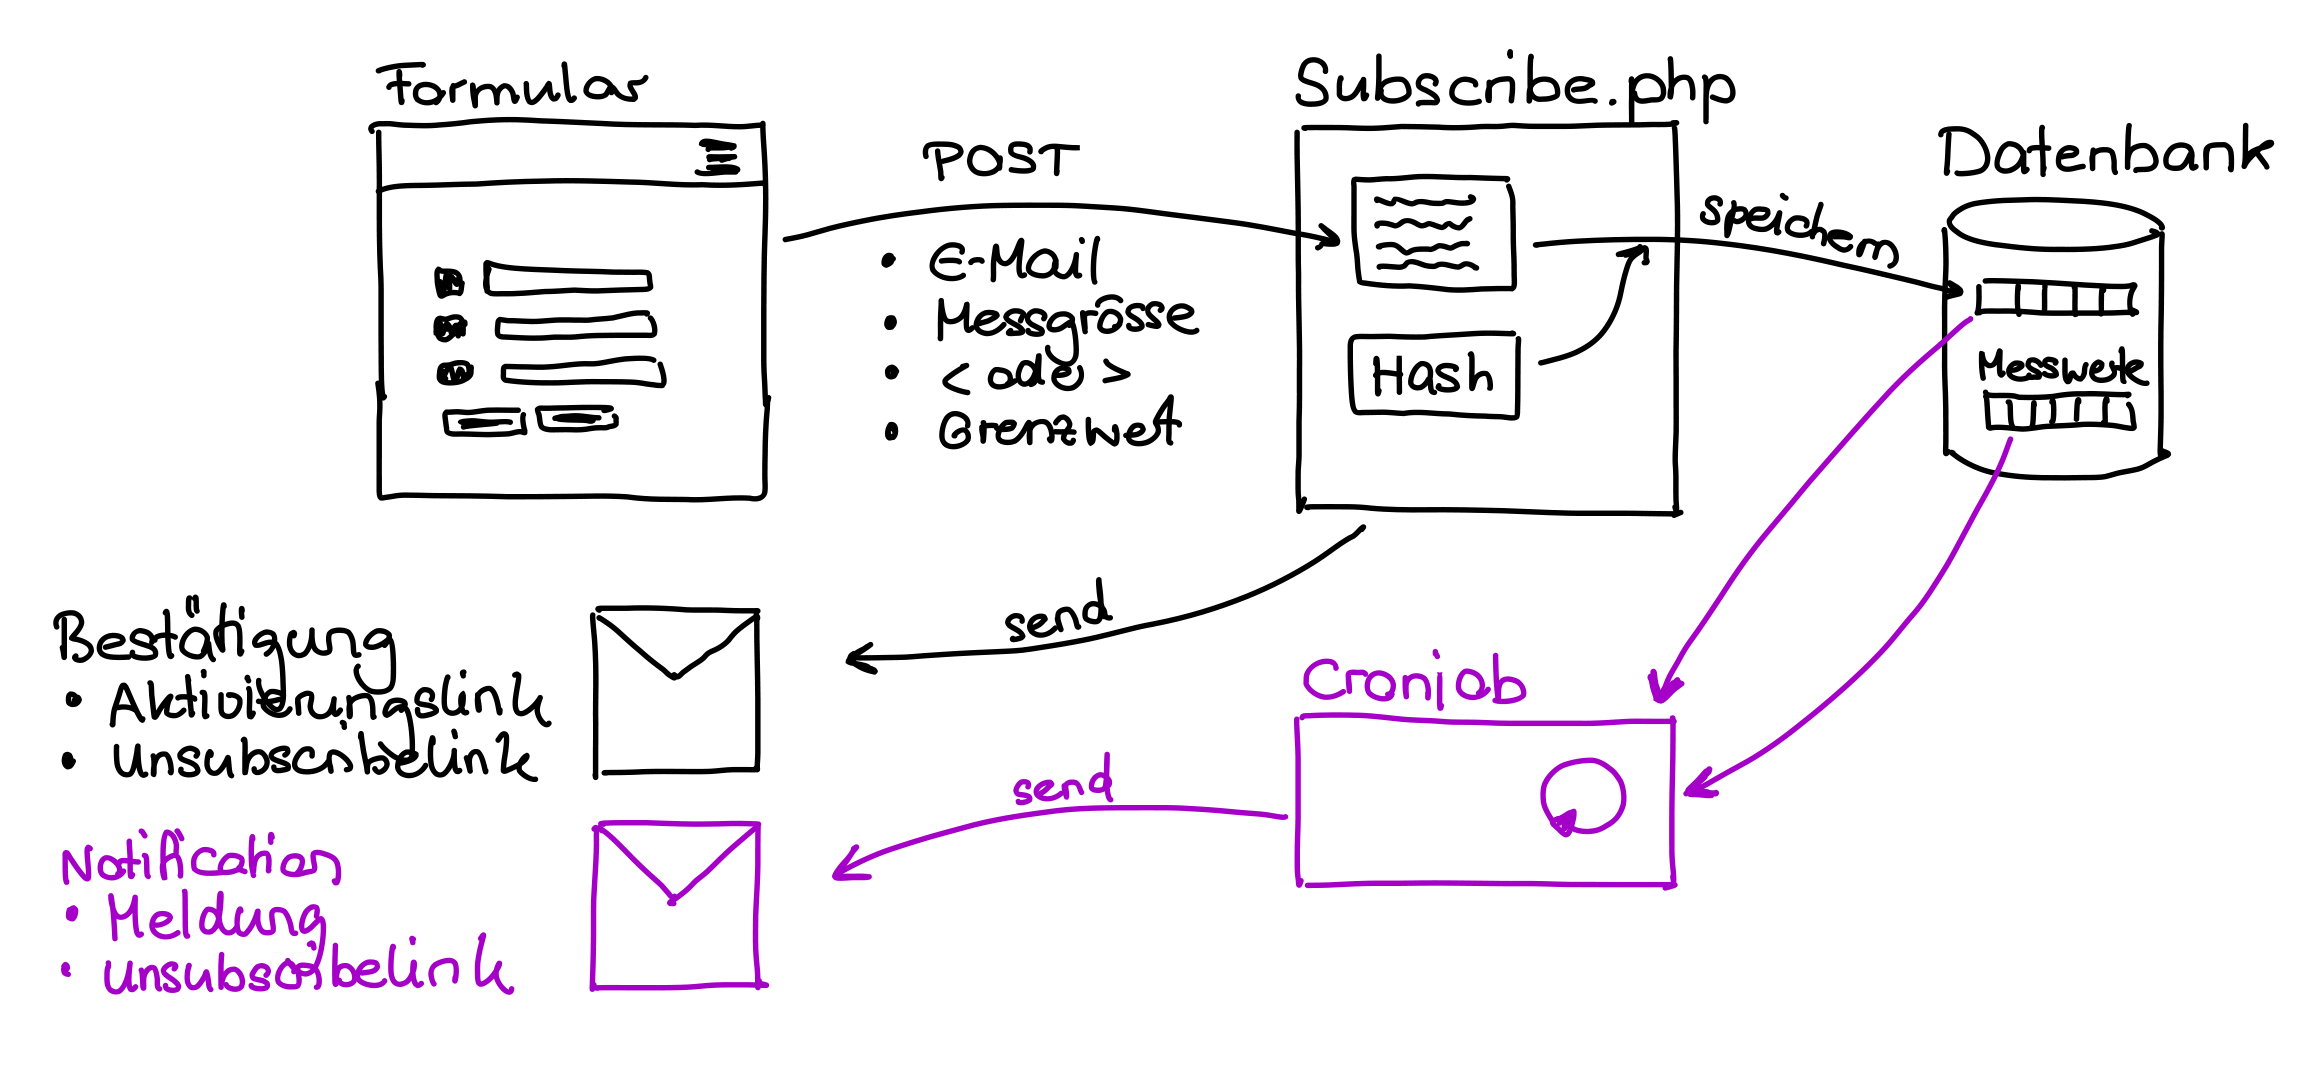
\includegraphics[width=\textwidth-2\fboxsep-2\fboxrule]{img/notificationKonzept}}
	\centering
	\caption{Funktionsprinzip des Benachrichtungsservices}
	\label{img:notificationKonzept}
\end{figure}

Der Benachrichtungsservice selbst basiert auf einem Cronjob, der einmal pro Stunde läuft. Das Prinzip ist in Abbildung \ref{img/notificationKonzept} in violett dargestellt. Der Cronjob ruft sämtliche Einträge in der Notification-Tabell ab und vergleicht sie mit den Messwerten. Sobald eine Bedingung erfüllt ist, wir ein Notification-Mail an die hinterlegete E-Mail-Adresse gesendet. Neben der eigentlichen Meldung ist ein Unsubscribelink vorhanden, damit der Benutzer den Benachritigungsservice abbestellen kann.

%% ###################################################################################################
%%   Unterkapitel                                                                                                                                                                              #
%% ###################################################################################################
\subsection{Formular mit integrierter Überprüfung der Eingabe}
Das Formular des Benachrichtungsservices besteht aus vier Eingabe- bzw. Auswahlfeldern, wie in Abbildung \ref{img/notificationFE}, links, dargestellt. Zuoberst kann die gewünschte Messgrösse ausgewählt werden. Das Dropdown-Menü stellt sicher, dass nur Werte ausgewählt werden können, die von der Wetterstation zur Verfügung gestellt werden. Mit den Radio-Buttons kann ausgewält werden ob der Messwert grösser oder kleiner als der Grenzwert sein soll. Der Grenzwert wird als Zahl eingeben auf eine Stelle nach dem Komma genau. Zuletzt muss die E-Mail-Adresse, an welche die Benachrichtigung gesendet werden soll eingetragen werden. Durch Anklicken des Abonnieren-Buttons wird das Formular abgesendet.

\begin{figure}[h!]
  \fbox{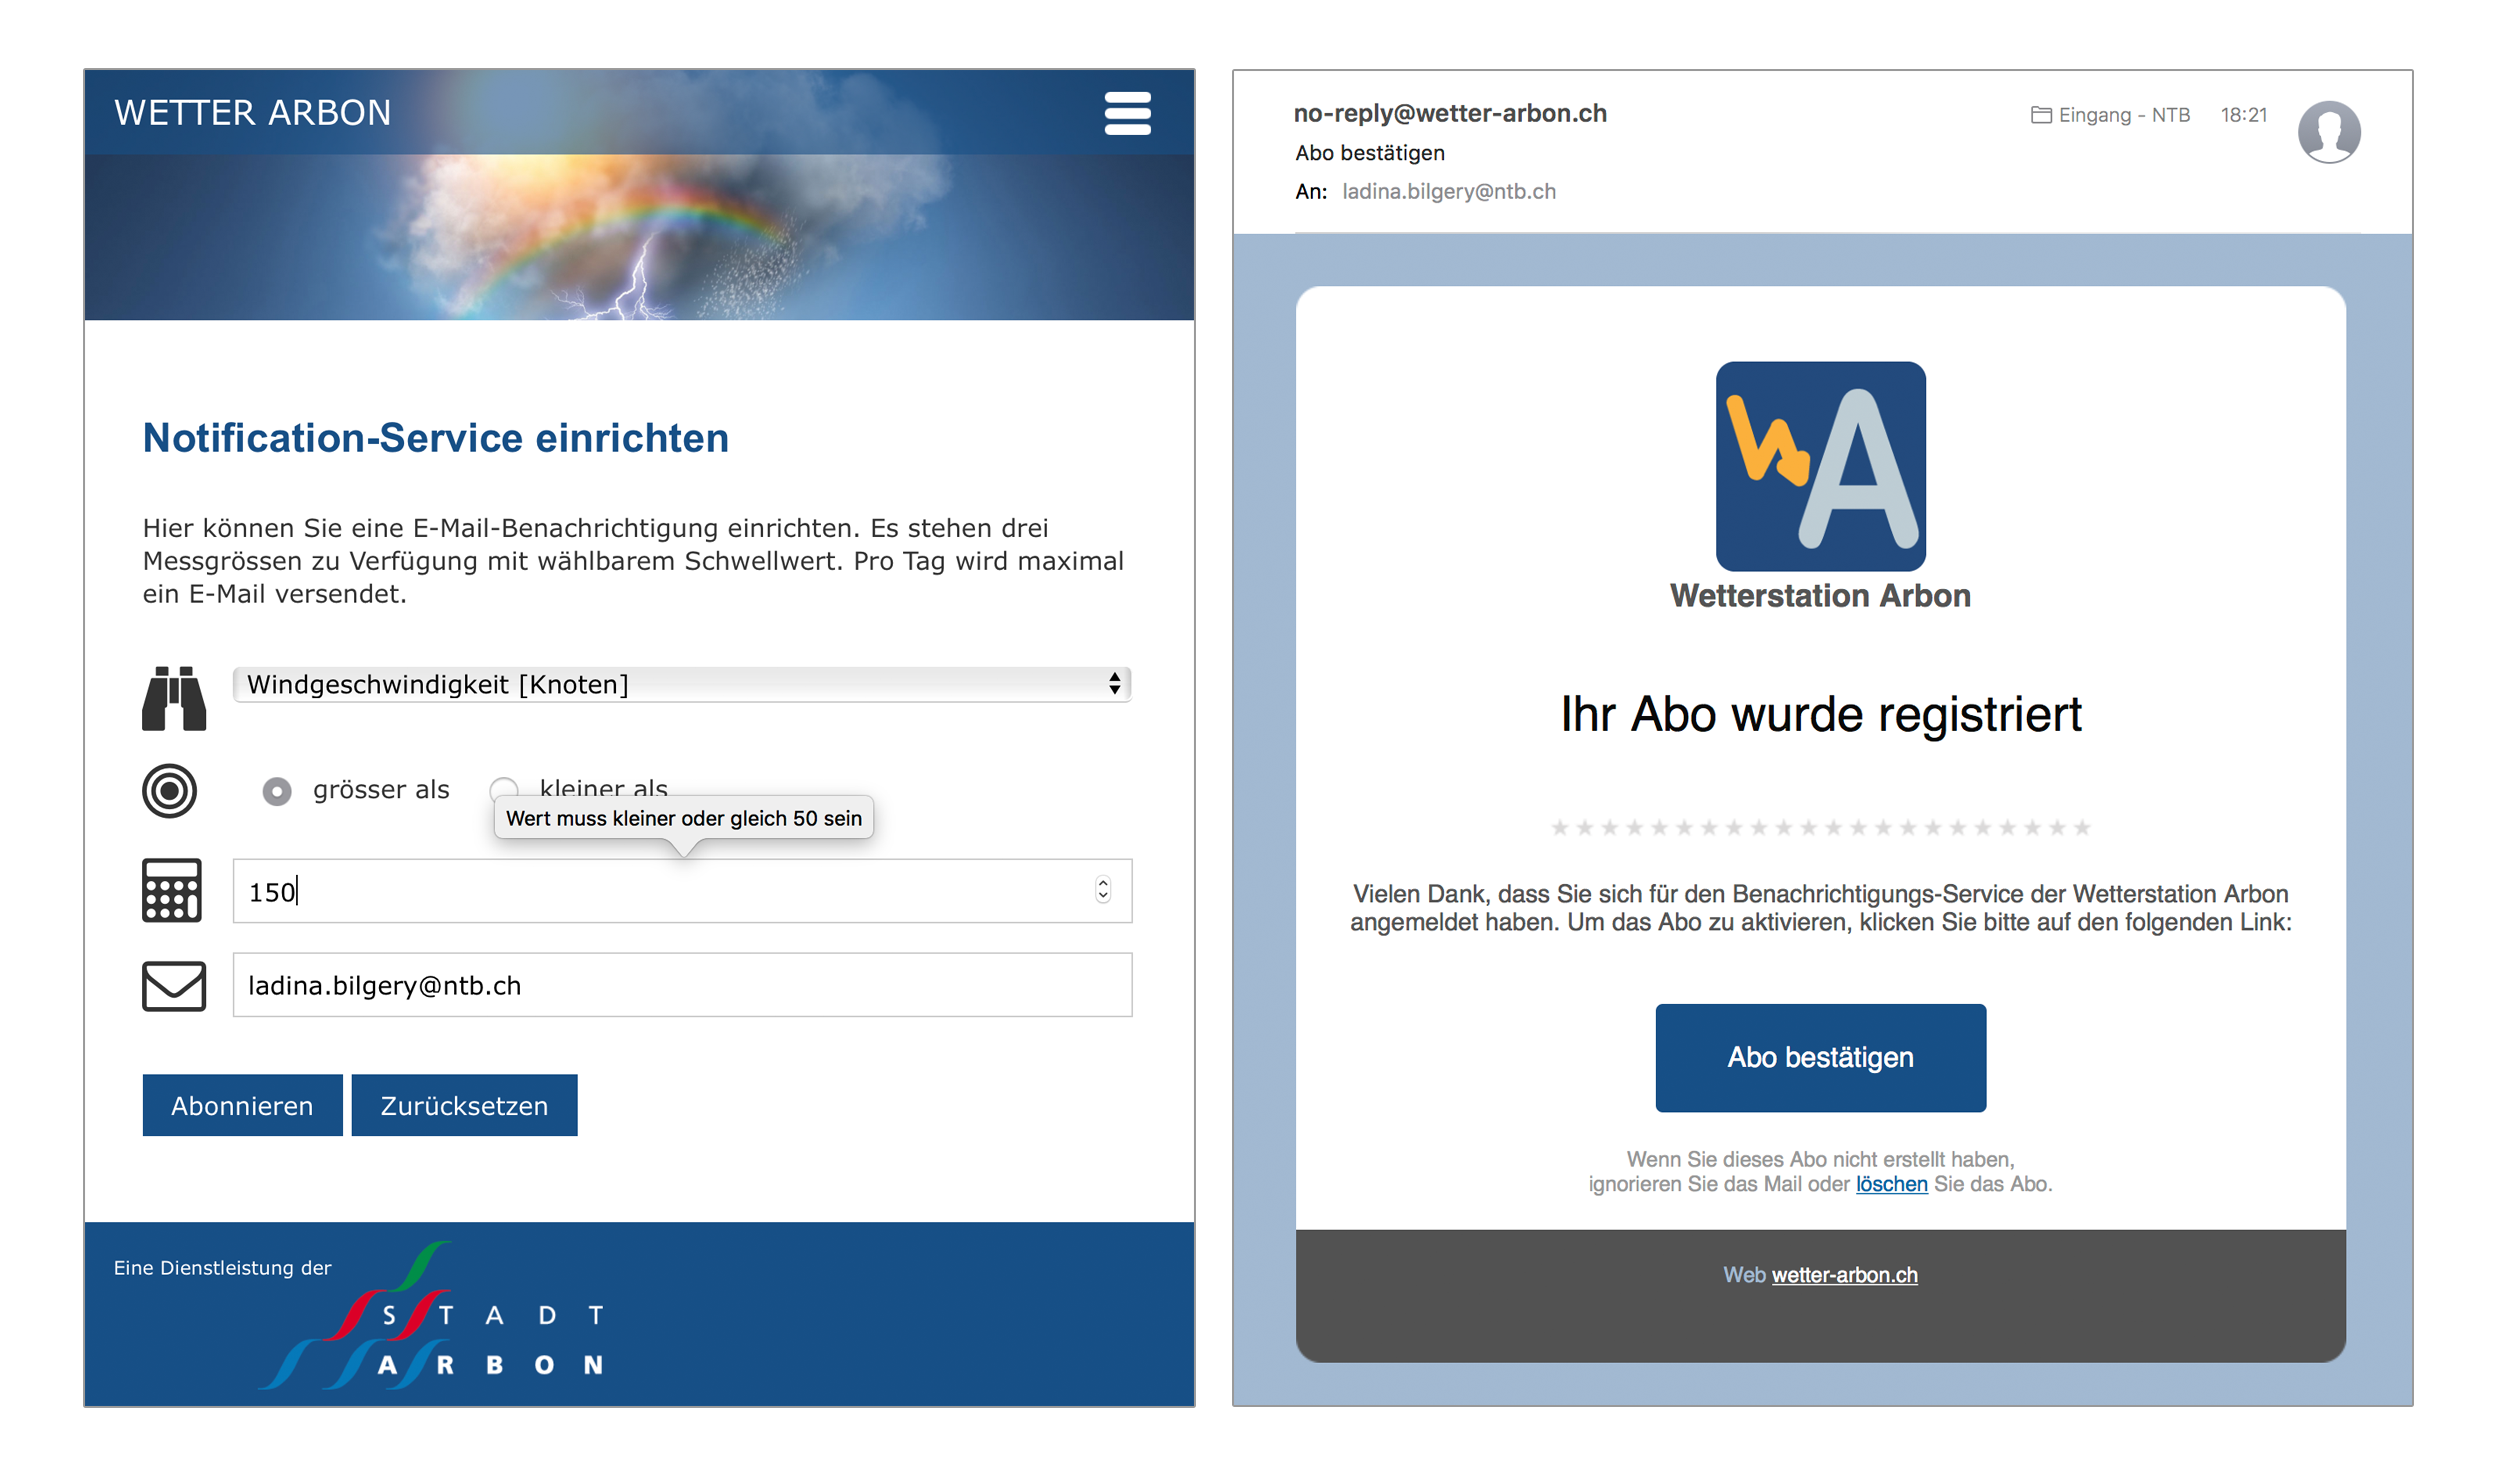
\includegraphics[width=\textwidth-2\fboxsep-2\fboxrule]{img/notificationFE}}
	\centering
	\caption{Eingabeformular mit Fehlerüberprüfung (rechts)}
	\label{img:notificationFE}
\end{figure}

Bisher musst die clientseitige Formularüberprüfung manuell programmierte werden bzw. eine JavaScript-Bibliothek verwendet werden. Unter HTML5 ist die Formularüberprüfung direkt integriert. Über die Defintion des \textit{type} und gegebenenfalls einiger Zusatzangaben, wird die  Überprüfung automtisch beim Absenden des Formulars durchgeführt und bei Fehlern direkt eine Meldung angezeigt. Der Wertebereich auf unsere Webseite ist zum Beispiel eingeschränkt auf Zahlen von 1 bis 50, wie in Listing \ref{lst:HTML5form} aufgezeigt. Wir nun ein Wert ausserhalb dieses Bereichs eingegeben, so erhält der Benutzer eine Fehlermeldung wie in Abbildung \ref{img/notificationFE}, rechts dargestellt und das Formular wird nicht abgesendet.

% Überprüfung der Eingaben
\begin{lstlisting}[label=lst:HTML5form,caption=Integrierte Formularüberprüfung mit HTML5, language=HTML5, style=htmlcssjs]
<!-- Auswahlmenue -->
<select name="measurand" required>
  <option value="" disabled selected>Messgrösse auswählen</option>
  <option value="windspeed">Windgeschwindigkeit</option>
</select>

<!-- Radio Button -->
<input type="radio" value="greater" checked>

<!-- Zahlenbereich -->
<input type="number" min="1" step="0.1" max="50" value="6">

<!-- E-Mail Adresse -->
<input type="email" placeholder="max.mustermann@web.ch" required>
\end{lstlisting}



%% ###################################################################################################
%%   Unterkapitel                                                                                                                                                                              #
%% ###################################################################################################
\subsection{Identificaiton des Abos via URL}
Die Tabelle für die Speicherung der Abos in der Datenbank enthält neben den vom Benutzer eingegbenen Daten noch weitere Einträge. Dies ist einerseits der Status des Abos d.h. aktiv oder inaktiv, den Zeitstempel des letzen Mails, sodass maximal einmal pro Tag ein Mail versendet wird, sowie den eindeutigen, nicht erratbaren Schlüssel (Hash), welcher für sämtliche Datenbank-Operationen benötigt wird.

% Bilder der DB-Tabellenstruktur?

Neben der \textit{subscribe.php}-Seite gibt es noch eine \textit{verify.php}-Seite und eine \textit{unsubscribe.php}-Seite. Diese führen jeweils die gewünschten Änderungen in der Datenbank aus. Zur Identifizierung des Abos enthält der Link sowohl die E-Mail-Adresse, als auch den Schlüssel (Hash) des entsprechenden Abos. Der Link für die Aktivierung des Abos lautet beispielhaft wie in Listing \ref{lst:verify} aufgeführt.

\begin{lstlisting}[label=lst:verify,caption=Beispiellink für die Aktivierung eines Abos, language=Python, style=py]
https://dev.wetter-arbon.ch/application/php/verify.php?
email=ladina.bilgery@ntb.ch&
hash=81f27f8a7d8766c72c0307a31327c1fad9007c6c3d33724ad2a5c0a8fe0df33d
\end{lstlisting}

Auf diese Weise kann auf Grund der aufgerufen Seite (subscribe, verify, unsubscribe) und dem Paar E-Mail und Schlüssel die Datenbankoperation genau definiert werden.

\section{Warteschlange-Funktion  für die Webcam}

Die Warteschlange sollte verhindern, dass mehrere Benutzer gleichzeitig die Webcam bedienen. Jeder der die Webcam bedienen möchte soll sich in einer Warteschlange registrieren. Ist diese erfolgt und der Benutzer an der Reihe, hat er 40 Sekunden Zeit die Webcam zu bedienen. Die Registrierung soll über einen Button Registrieren erfolgen. Die Warteschlange funktioniert folgendermassen, registriert sich ein Benutzer per Klick auf den Registrierungsbutton wird eine Sessionid gelöst. Anschliessend wird in der Datenbank abgefragt ob weitere Benutzer in der Warteschlange sind. Hierbei bestehen zwei Möglichkeiten:\\

Keine weiteren Benutzer:\\
Die Session ID mit dem Zeitstempel und der Wartezeit für den nächsten wird in die Datenbank geschrieben. Dies ist in Bild \ref{img:tblqueue} zu sehen.
\begin{figure}[h!]
  \fbox{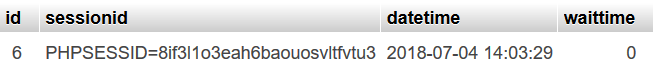
\includegraphics[width=\textwidth-2\fboxsep-2\fboxrule]{img/tblqueue.png}}
	\centering
	\caption{Datenbankeintrag, wenn keine weiteren Benutzer in der Warteschlange sind}
	\label{img:tblqueue}
\end{figure}

Der registrierte Benutzer bekommt Zugriff auf die Navigationstools der Webcam. Nach der Nutzzeit werden die Tools wieder deaktiviert, sodass ein bedienen der Webcam nicht möglich ist. 
Vorgehen mehrere Benutzer:\\

Sind mehrere Benutzer in der Warteschlange wird die Wartezeit in Sekunden angezeigt. 
\begin{figure}[h!]
  \fbox{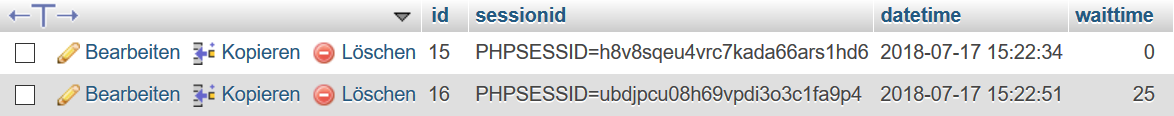
\includegraphics[width=\textwidth-2\fboxsep-2\fboxrule]{img/tblqueuemitBenutzer.png}}
	\centering
	\caption{Datenbankeintrag, mehrere Benutzer registriert sind}
	\label{img:tblqueue}
\end{figure}


\newpage
% braucht es das?
\FloatBarrier

\newpage
\pagestyle{plain}
\input{schluss}
\newpage
\bibliography{literatur}{}
\bibliographystyle{plain}
\newpage

\appendix
\section{Schemata}

\begin{itemize}
	\item Schema aller Geräte
	\item Datenbankschema komplett
	\item Schema Aufbau Back end
	\item Schema Aufbau Webseite (screenbox)
\end{itemize}

\newpage
\section{Source code}

\subsection{JSON-Tree}

\begin{lstlisting}[label=lst:JsonTree,caption=Json Struktur, language=JavaScript, style=htmlcssjs, mathescape]
{
  "product": "api.wetter-arbon.ch",
  "version": "1.1.1",
	{
    "v1": {
        "misc": {
            "west": {
                "description": "Warnlevel west",
                "warnlevel": 40,
                "onset": "2018-07-17 13:05:00",
                "expires": null,
                "timestamp": "2018-07-17 13:24:00",
                "interval": 60,
                "intervalUnit": "seconds"
            },
            "middle": {
                "description": "Warnlevel middle",
                "warnlevel": 40,
                "onset": "2018-07-17 13:06:00",
                "expires": null,
                "timestamp": "2018-07-17 13:24:00",
                "interval": 60,
                "intervalUnit": "seconds"
            },
            "east": {
                "description": "Warnlevel east",
                "warnlevel": 0,
                "onset": null,
                "expires": null,
                "timestamp": "2018-07-17 13:24:00",
                "interval": 60,
                "intervalUnit": "seconds"
            }
        },
        "webcam": {
            "name": "Webcam Wetter Arbon",
            "title": "webcam",
            "url": "https://webcam.wetter-arbon.ch/mjpg/video.mjpg"
        },
        "data": {
            "temperature": {
                "description": "Lufttemperatur",
                "unit": "${^\circ}$C",
                "value": 22.6,
                "dailymax": 22.6,
                "dailymin": 17,
                "timestamp": "2018-07-17 13:24:31",
                "interval": 60,
                "intervalUnit": "seconds"
            },
            "windchill": {
                "description": "Windchill",
                "unit": "${^\circ}$C",
                "value": 22.6,
                "dailymax": 22.6,
                "dailymin": 17,
                "timestamp": "2018-07-17 13:24:31",
                "interval": 60,
                "intervalUnit": "seconds"
            },
            "humidity": {
                "description": "Relative Luftfeuchtigkeit",
                "unit": "%",
                "value": 60,
                "timestamp": "2018-07-17 13:24:31",
                "interval": 60,
                "intervalUnit": "seconds"
            },
            "winddirection": {
                "description": "Windrichtung",
                "unit": "${^\circ}$",
                "value": 75,
                "timestamp": "2018-07-17 13:24:31",
                "interval": 60,
                "intervalUnit": "seconds"
            },
            "windspeed": {
                "knoten": {
                    "value": 7.6,
                    "dailymax": 7.9,
                    "unit": "kn"
                },
                "kmph": {
                    "value": 14.08,
                    "dailymax": 14.63,
                    "unit": "km/h"
                },
                "beaufort": {
                    "value": 3,
                    "dailymax": 3,
                    "unit": "Bft"
                },
                "description": "Windgeschwindigkeit",
                "timestamp": "2018-07-17 13:24:31",
                "interval": 60,
                "intervalUnit": "seconds"
            },
            "gust": {
                "knoten": {
                    "value": 8,
                    "dailymax": 8.2,
                    "unit": "kn"
                },
                "kmph": {
                    "value": 14.82,
                    "dailymax": 15.19,
                    "unit": "km/h"
                },
                "beaufort": {
                    "value": 3,
                    "dailymax": 3,
                    "unit": "Bft"
                },
                "description": "Böen",
                "unit": "kn",
                "timestamp": "2018-07-17 13:24:31",
                "interval": 60,
                "intervalUnit": "seconds"
            },
            "precipitation": {
                "description": "Niederschlagsmenge seit Mitternacht",
                "unit": "mm",
                "value": 0,
                "timestamp": "2018-07-17 13:24:31",
                "interval": 60,
                "intervalUnit": "seconds"
            },
            "pressure": {
                "description": "Luftdruck",
                "unit": "hPa",
                "value": 1017.1,
                "timestamp": "2018-07-17 13:24:31",
                "interval": 60,
                "intervalUnit": "seconds"
            },
            "weathericon": {
                "description": "Icon type current weather",
                "value": 5,
                "timestamp": "2018-07-17 13:24:31",
                "interval": 60,
                "intervalUnit": "seconds"
            },
            "forecasticon": {
                "description": "Forecast icon",
                "value": 5,
                "timestamp": "2018-07-17 13:24:31",
                "interval": 60,
                "intervalUnit": "seconds"
            },
            "watertemperature1m": {
                "description": "Wassertemperatur 1m unter der Wasseroberfläche",
                "unit": "${^\circ}$C",
                "value": 24.2,
                "timestamp": "2018-07-17 13:24:00",
                "interval": 60,
                "intervalUnit": "seconds"
            },
            "watertemperature0m5": {
                "description": "Wassertemperatur 0.5m unter der Wasseroberfläche",
                "unit": "${^\circ}$C",
                "value": 23.9,
                "timestamp": "2018-07-17 13:24:00",
                "interval": 60,
                "intervalUnit": "seconds"
            },
            "waterlevel": {
                "description": "Bodenseepegel",
                "unit": "m",
                "value": 3.54,
                "timestamp": "2018-07-17 13:24:00",
                "interval": 60,
                "intervalUnit": "seconds"
            },
            "radiation": {
                "description": "Globalstrahlung",
                "unit": "W/m2",
                "value": 868,
                "timestamp": "2018-07-17 13:24:00",
                "interval": 60,
                "intervalUnit": "seconds"
            },
            "sunduration": {
                "description": "Sonnenstunden",
                "unit": "h/d",
                "value": 5,
                "timestamp": "2018-07-17 13:24:00",
                "interval": 60,
                "intervalUnit": "seconds"
            }
        }
    }
}
}
\end{lstlisting}

\subsection{Datenbankcode}\label{anhang:Datenbankcode}
\begin{itemize}
	\item API
	\item Links? (URL, Git, GitPages, usw.)
\end{itemize}

\newpage
\section{Datenblätter}
%\addcontentsline{toc}{section}{Datenblätter}

%Pegelsensors
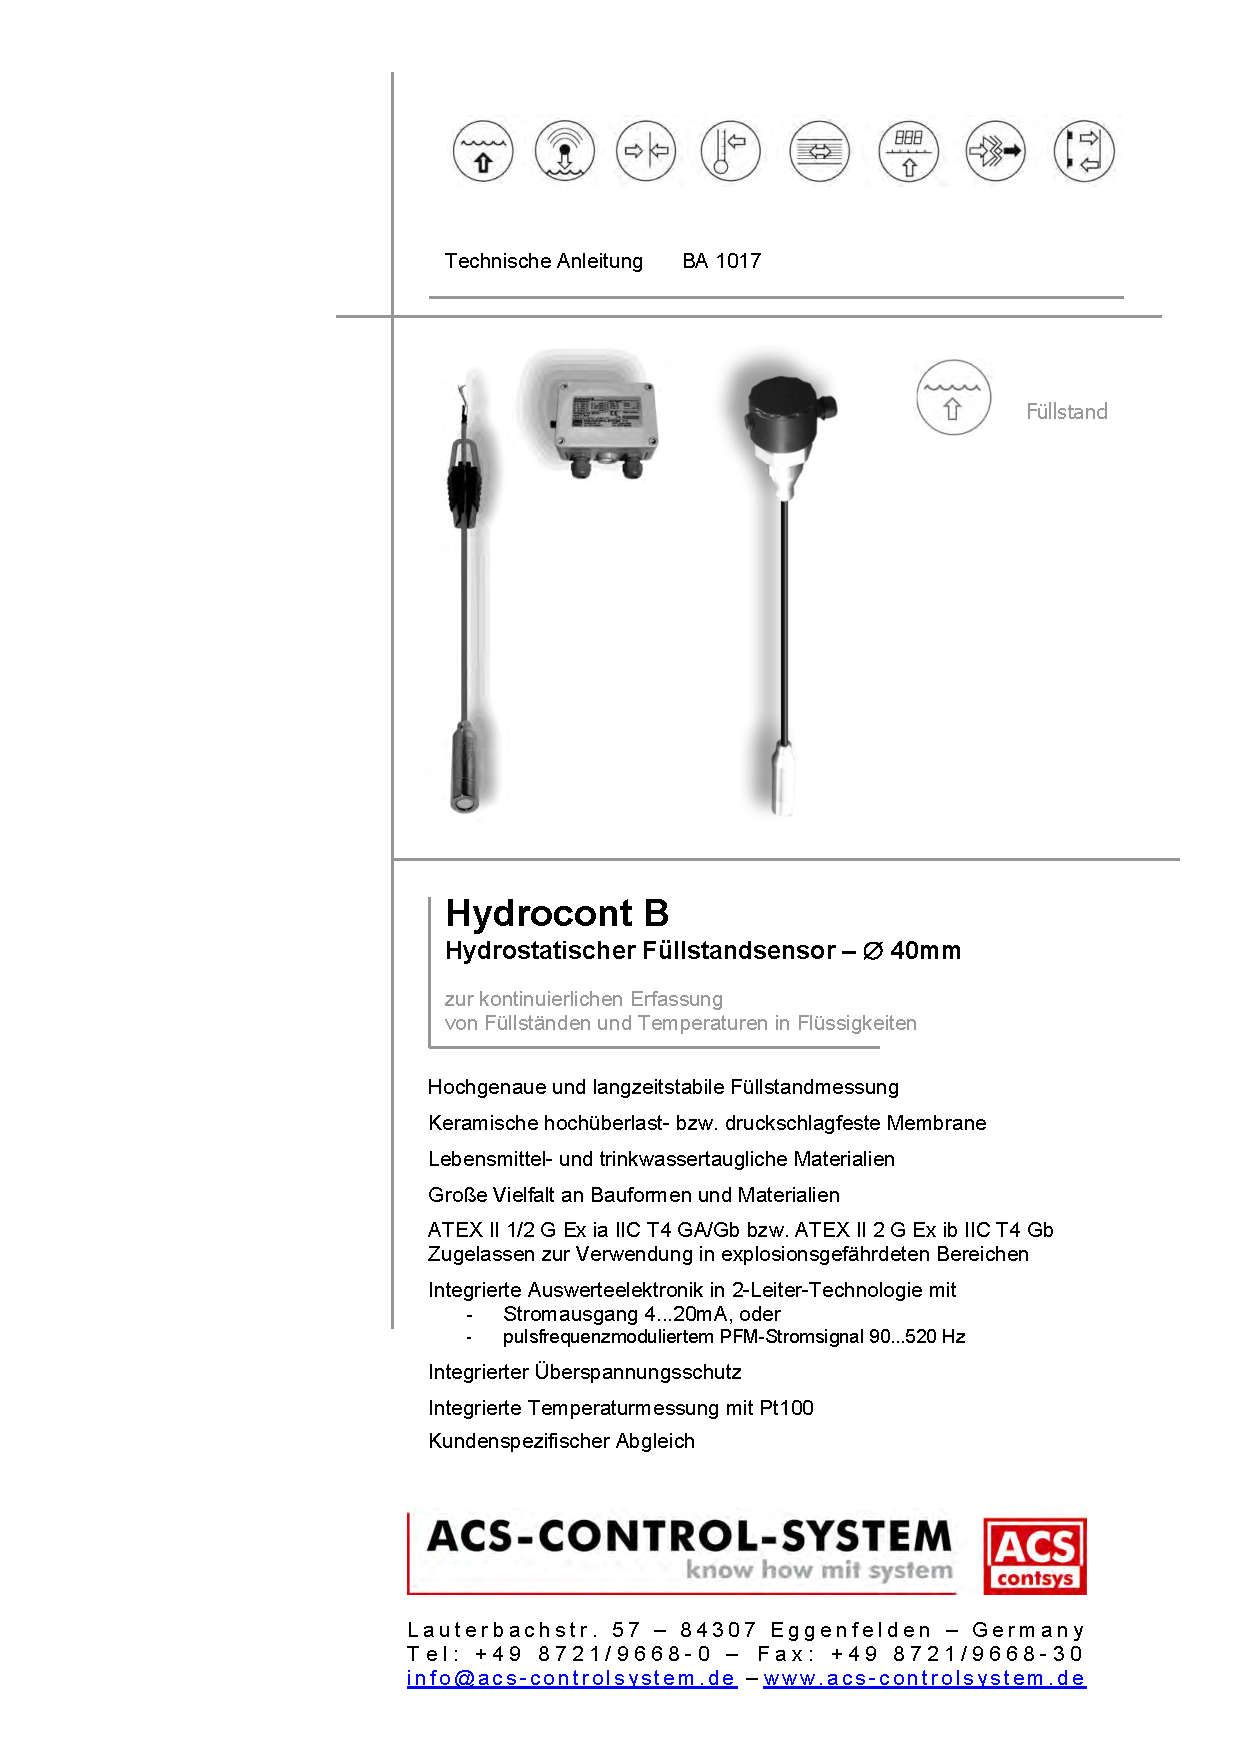
\includepdf[pages=1,frame,scale=0.7,pagecommand={\pagestyle{plain}\subsection{Pegelsensor}}]{appendix/Spec_HydrocontB.pdf}
\includepdf[pages=2-,frame,scale=0.7,pagecommand={}]{appendix/Spec_HydrocontB.pdf}

% Strahlungssensor
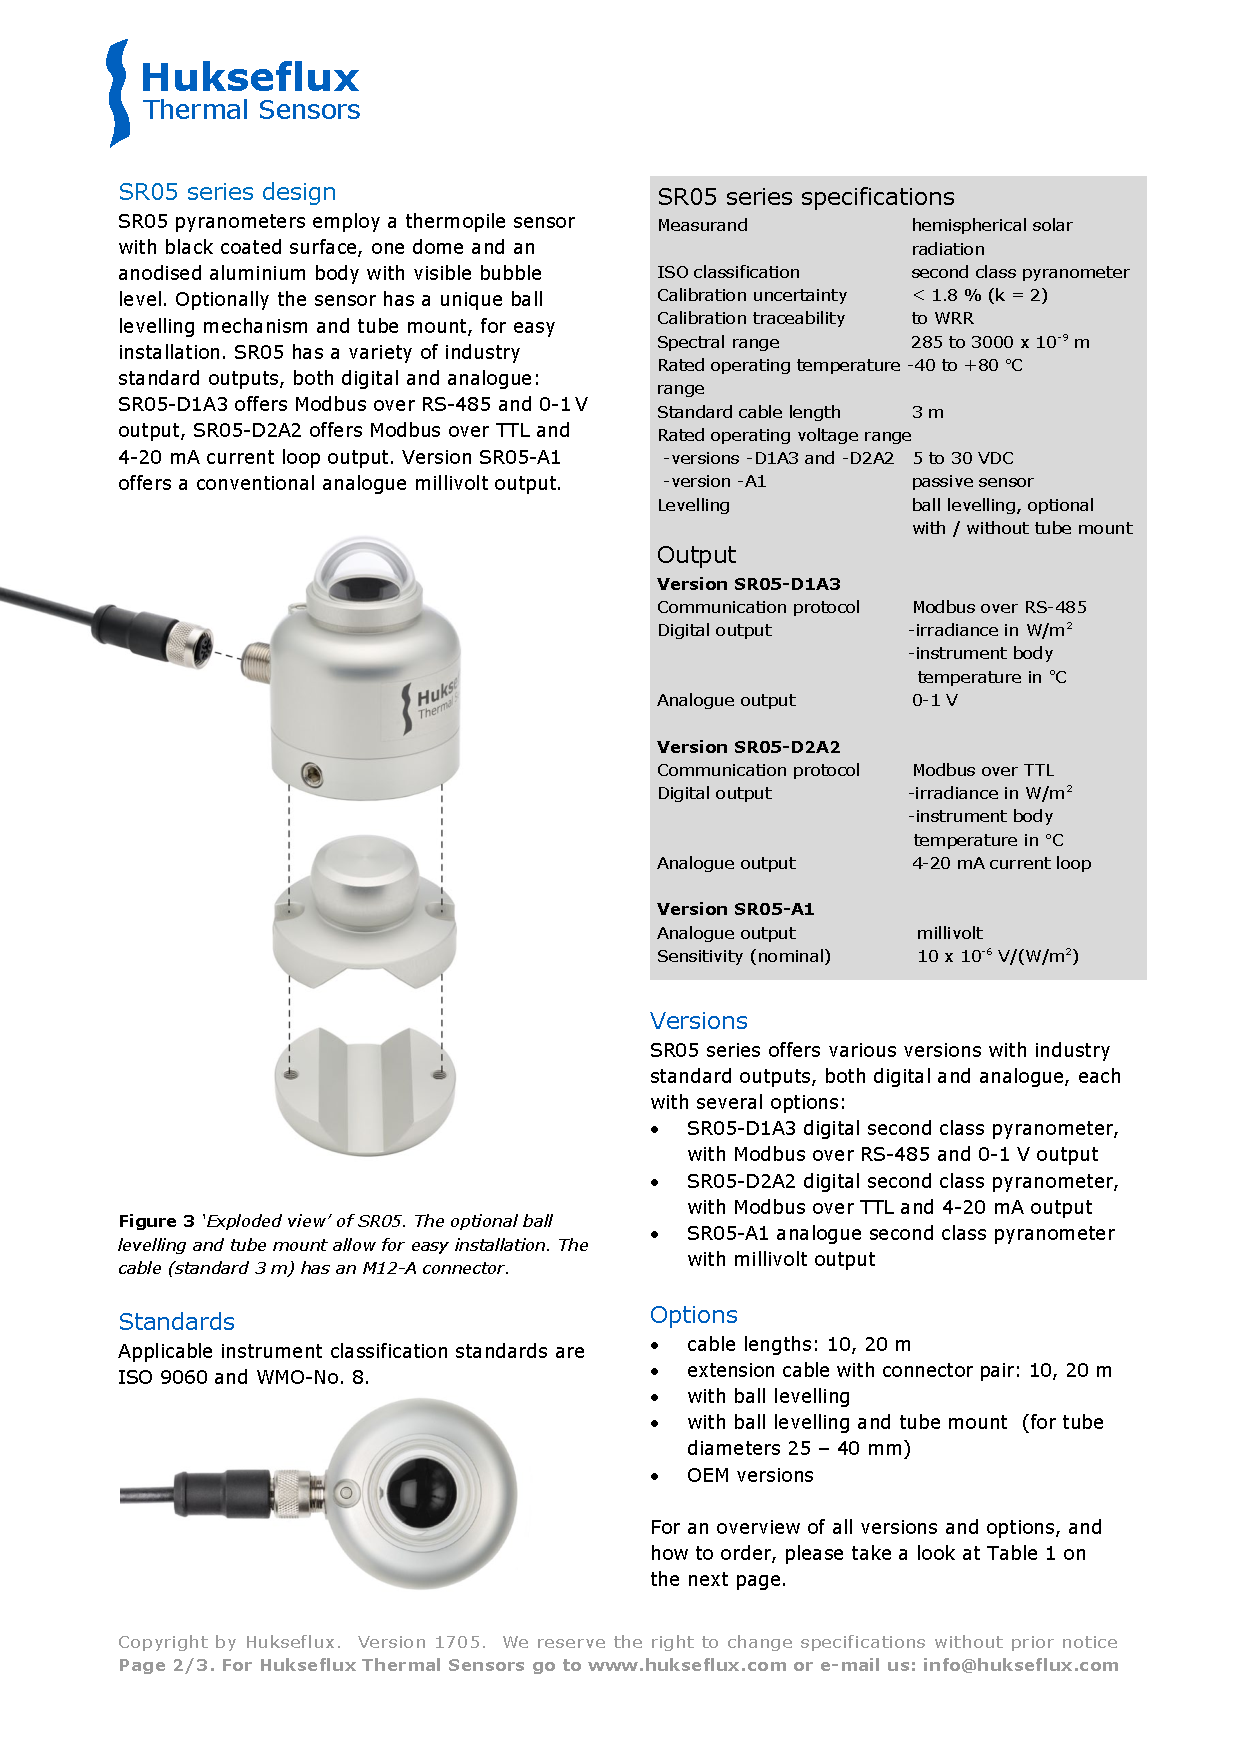
\includepdf[pages=-,frame,scale=0.7,pagecommand={\pagestyle{plain}\subsection{Strahlungssensor}}]{appendix/Spec_SR05.pdf}

% Web Thermograph
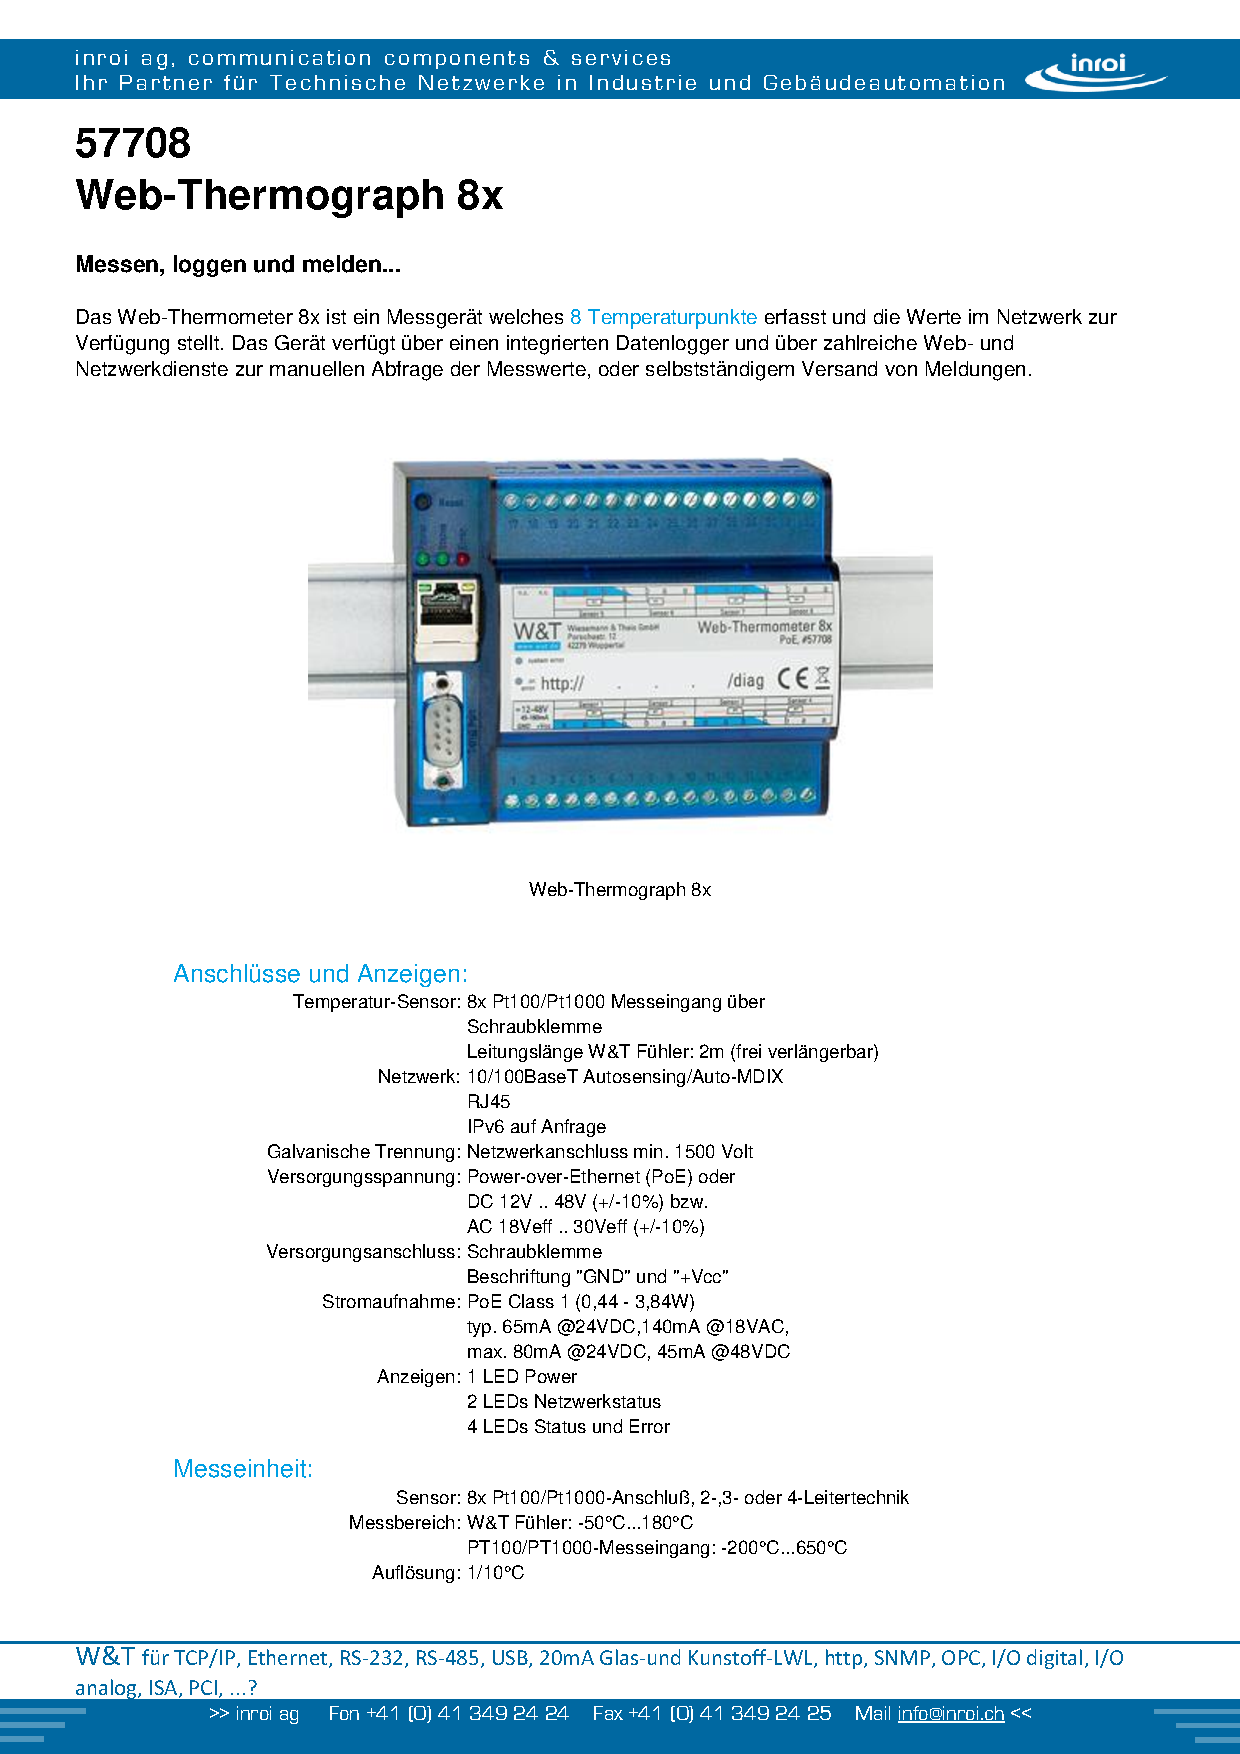
\includepdf[pages=1,frame,scale=0.7,pagecommand={\pagestyle{plain}\subsection{Web-Thermograph 8x}}]{appendix/Spec_WTthermo.pdf}
\includepdf[pages=2-,frame,scale=0.7,pagecommand={}]{appendix/Spec_WTthermo.pdf}

% Web-IO
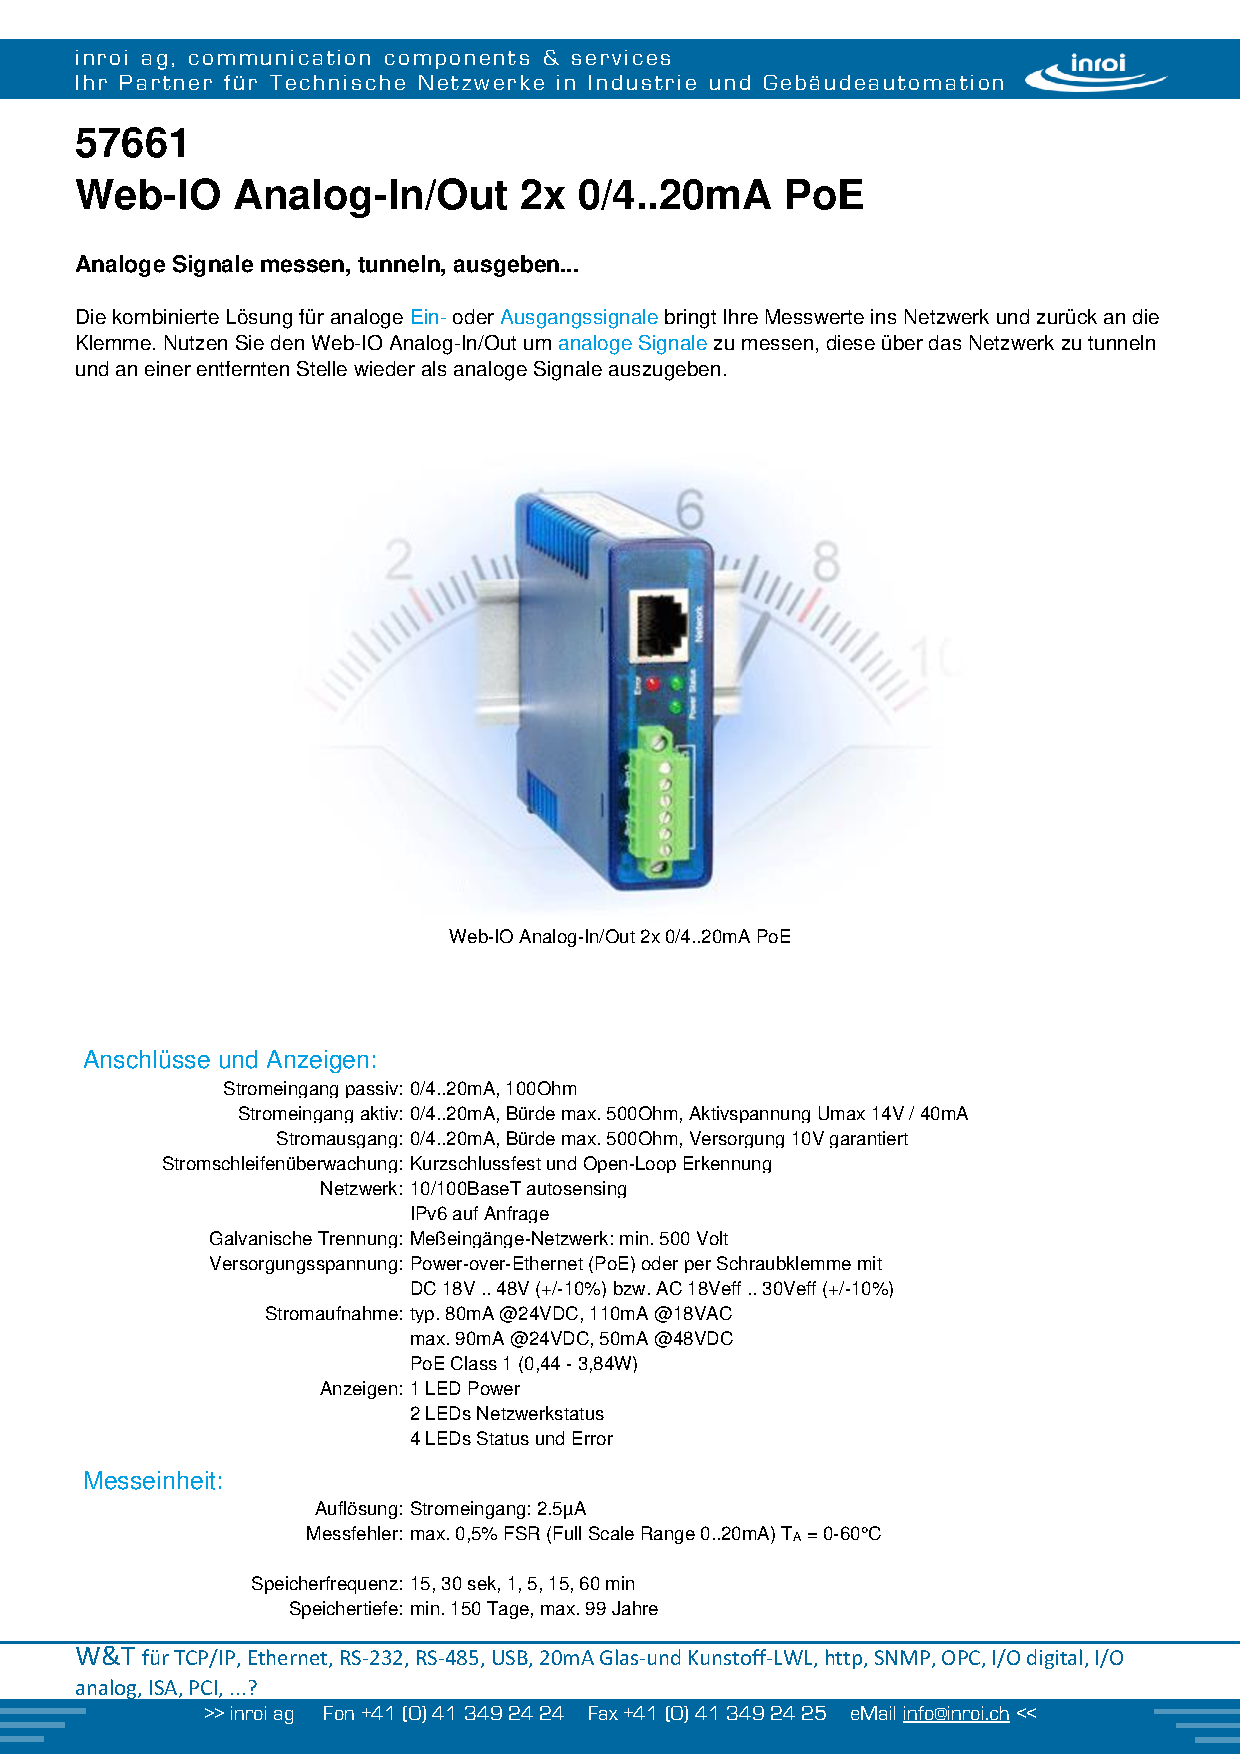
\includepdf[pages=1 ,frame,scale=0.7,pagecommand={\subsection{Web-IO Analog-In/Out 2x}}]{appendix/Spec_WTanalog.pdf}
\includepdf[pages=2-,frame,scale=0.7,pagecommand={}]{appendix/Spec_WTanalog.pdf}

\newpage


\end{document}
